% Compile with LuaLaTeX, Biber, then LuaLaTeX twice.
\documentclass[12pt,a4paper]{article}
\usepackage[margin=27mm,headheight=15pt,headsep=7mm]{geometry}
\usepackage{fontspec}
\setmainfont{STIXTwoText}[
 Path=fonts/,Extension=.ttf,UprightFont=*-Regular,ItalicFont=*-Italic,
 BoldFont=*-Bold,BoldItalicFont=*-BoldItalic]
\usepackage{amsmath,amsthm,mathtools}
\usepackage{unicode-math}
\setmathfont{STIXTwoMath-Regular.otf}[Path=fonts/]
\usepackage{microtype}
\usepackage{xcolor,graphicx,booktabs,array,longtable}
\usepackage{enumitem}
\usepackage{caption}
\usepackage{fancyhdr}
\usepackage{needspace}
\usepackage{etoolbox}
\usepackage{csquotes}
\definecolor{ink}{HTML}{202A34}
\definecolor{teal}{HTML}{167B80}
\definecolor{rust}{HTML}{B35732}
\usepackage[
 backend=biber,style=numeric,sorting=nyt,giveninits=true,
 maxbibnames=8,doi=true,url=true,isbn=false,eprint=true
]{biblatex}
\addbibresource{references.bib}
\usepackage[colorlinks=true,linkcolor=teal,citecolor=teal,urlcolor=teal,
 pdftitle={The constant, the curve and a paradox},
 pdfauthor={Sol, Astra and Captain Sude},
 pdfsubject={Arithmetic information in digits, probability and graphs},
 bookmarksnumbered=true]{hyperref}
\usepackage{bookmark}
\linespread{1.08}
\setlength{\parskip}{4pt}
\setlength{\parindent}{1em}
\setlength{\emergencystretch}{2em}
\setlength{\textfloatsep}{16pt plus 3pt minus 3pt}
\captionsetup{font=small,labelfont=bf,justification=justified}
\setlist{itemsep=3pt,topsep=5pt}
\setcounter{tocdepth}{1}
\numberwithin{equation}{section}
\newtheoremstyle{readable}{10pt}{8pt}{\normalfont}{}{\bfseries}{.}{.6em}{}
\theoremstyle{readable}
\newtheorem{theorem}{Theorem}[section]
\newtheorem{proposition}[theorem]{Proposition}
\newtheorem{lemma}[theorem]{Lemma}
\newtheorem{corollary}[theorem]{Corollary}
\theoremstyle{definition}
\newtheorem{definition}[theorem]{Definition}
\theoremstyle{remark}
\newtheorem{remark}[theorem]{Remark}
\newtheorem{example}[theorem]{Example}
\newtheorem{question}[theorem]{Question}
\newtheorem{conjecture}[theorem]{Conjecture}
\newcommand{\E}{\mathbb E}
\newcommand{\Prob}{\mathbb P}
\newcommand{\Gold}{\mathcal G}
\newcommand{\Comp}{W_{\mathrm c}}
\newcommand{\CompN}{W_{\mathrm c,N}}
\newcommand{\SymCDF}{F_{\mathrm{sym}}}
\newcommand{\GC}{\mathrm{Goldbach}}
\newcommand{\RH}{\mathrm{RH}}
\DeclareMathOperator{\lpf}{lpf}
\DeclareMathOperator{\rad}{rad}
\DeclareMathOperator{\Var}{Var}
\DeclareMathOperator{\Cov}{Cov}
\DeclareMathOperator{\TV}{TV}
\DeclareMathOperator{\supp}{supp}
\DeclareMathOperator{\tr}{tr}
\newcommand{\ind}{\mathbf 1}
\newcommand{\dd}{\,d}
\pagestyle{fancy}
\fancyhf{}
\fancyhead[L]{\small\itshape The constant, the curve and a paradox}
\fancyhead[R]{\small Sol, Astra and Captain Sude}
\fancyfoot[C]{\small\thepage}
\renewcommand{\headrulewidth}{0.3pt}
\renewcommand{\sectionmark}[1]{\markboth{#1}{}}
\AtBeginEnvironment{theorem}{\Needspace{5\baselineskip}}
\AtBeginEnvironment{proposition}{\Needspace{5\baselineskip}}
\AtBeginEnvironment{lemma}{\Needspace{5\baselineskip}}
\AtBeginEnvironment{corollary}{\Needspace{5\baselineskip}}
\title{\LARGE The constant, the curve\\[3pt] and a paradox\\[9pt]
 \large Arithmetic information in digits, probability and graphs}
\author{Sol \and Astra \and Captain Sude}
\date{\small 25 September 2026}
\begin{document}
\color{ink}
\pagenumbering{roman}
\begin{titlepage}
\thispagestyle{empty}
\centering
\vspace*{34mm}
{\fontsize{30}{36}\selectfont
The constant, the curve\\[4pt]and a paradox\par}
\vspace{10mm}
{\large Arithmetic information in digits, probability and graphs\par}
\vspace{24mm}
{\large Sol \qquad Astra \qquad Captain Sude\par}
\vfill
{\small 25 September 2026\par}
\end{titlepage}
\setcounter{page}{2}
\begingroup
\small
\setlength{\parskip}{0pt}
\linespread{1}\selectfont
\makeatletter
\patchcmd{\l@section}{1.0em}{0.65em}{}{}
\makeatother
\tableofcontents
\endgroup
\clearpage
\begingroup
\small
\section*{Symbols at a glance}
\phantomsection
\addcontentsline{toc}{section}{Symbols at a glance}
\label{app:notation}

Each object is introduced where it first appears; this page is a place
to return to. Here $p_j$ is the $j$th prime. The lane of $p$ consists
of integers whose least prime factor is $p$.

\renewcommand{\arraystretch}{1.35}
\begin{longtable}{@{}p{.23\linewidth}p{.72\linewidth}@{}}
\toprule
Symbol & Meaning \\
\midrule
\endhead
$\Gold$ & The original Goldbach constant. \\
$C_g$ & A constant carrying a binary message $g$:
$g_j=0$ closes the lane of $p_j$; $g_j=1$ opens it. \\
$x_g(n)$ & The $n$th binary digit of $C_g$. \\
$\ell(n)$ & For $n\ge2$, the index of its least prime factor:
$\lpf(n)=p_{\ell(n)}$. \\
$\lambda(n)$ & The Liouville sign, $(-1)^{\Omega(n)}$;
$\Omega$ counts prime factors with multiplicity. \\
$\delta_j$ & The density of positions in the lane of $p_j$. \\
$S_g$ & The total density of disabled lanes. \\
$M_k(g)$ & The correlation of $k$ signs $1-2x_g(n)$, conditioned on pairwise coprime digit positions. \\
$K(k)$ & The limiting probability that $k$ sampled integers are pairwise coprime. \\
$\Phi_g,\Psi_g$ & The generating functions for conditioned and unconditioned correlations, respectively. \\
$W,\Comp$ & Independent prime and composite random factors;
$W\Comp$ has the exponential law of mean one. \\
$f,\SymCDF$ & The density of $W$ on $(0,\infty)$, extended to the complex plane,
and the symmetric cumulative distribution function derived from it. \\
$G_g$ & The cumulative distribution function from sampling equally spaced
digit positions with coprime start and step. \\
$G_N,Y_N$ & The clean and observed labelled coprimality tables in the finite recovery experiment. \\
$T_N$ & Effective signal $N(1-2\varepsilon_N)^2$, where $\varepsilon_N$
is the probability of flipping each pair answer. \\
$D(n)$ & The effective count of prime-power parts $p^{v_p(n)}$,
measured by the entropy of their logarithmic shares. \\
$B_k$ & The set of primes still present after deletion round $k$. \\
\bottomrule
\end{longtable}
\renewcommand{\arraystretch}{1}

\noindent All logarithms are natural unless a base is specified.
Local cutoff variables are defined where used.

\endgroup
\clearpage
\pagenumbering{arabic}
\section{The constant: repeating the Goldbach questions}
\label{fnd:constant}

Goldbach's conjecture asks whether every even integer greater than two is a
sum of two primes.  We begin by making a real number that remembers all of
these questions.  List the primes as $p_1=2,p_2=3,p_3=5,\ldots$, and attach
the question about $2(j+1)$ to $p_j$.  Thus the prime $2$ carries the question
about $4$, the prime $3$ the question about $6$, and so on.  Write
\[
 g_j=\mathbf1_{\{2(j+1)\text{ is a sum of two primes}\}}.
\]
Putting $g_j$ only at digit position $p_j$ would hide the answers in a set
of density zero.  Instead, we repeat each answer along a whole
\emph{prime lane}: the positive integers whose least prime factor is $p_j$.

One further ingredient gives the number its internal arithmetic.  Let
$\Omega(n)$ count prime factors with multiplicity, let
$\lambda(n)=(-1)^{\Omega(n)}$, and set $\lambda(1)=1$.  For $n\ge2$ let
$\ell(n)$ be the index of its least prime factor.  Our constant is
\begin{equation}
 x_1=0,\qquad x_n=\frac{1-\lambda(n)}2g_{\ell(n)}\quad(n\ge2),
 \qquad \Gold=\sum_{n\ge1}x_n2^{-n}.
 \label{fnd:definition}
\end{equation}
Every digit is computable by a finite calculation.  In an enabled lane,
the digit is one when the number has an odd number of prime factors,
counting multiplicity.  In a disabled lane every digit is zero.
At prime positions the Liouville factor equals $-1$, so
\begin{equation}
 x_{p_j}=g_j.
 \label{fnd:prime-reading}
\end{equation}
The prime digits therefore list the Goldbach answers exactly, while the
other digits repeat those answers in a structured way.

It is useful to permit an arbitrary binary message
$g=(g_1,g_2,\ldots)$ in the same definition.  We write the resulting
digits as $x_g(n)$ and the resulting real as $C_g$.  Unless explicitly
stated otherwise, the family has $g_1=1$; the original $\Gold$ is its
Goldbach member.  We shall use
\begin{equation}
 h_g(1)=0,\qquad h_g(n)=1-g_{\ell(n)}\ (n\ge2),\qquad
 a_g(n)=1-2x_g(n)=h_g(n)+(1-h_g(n))\lambda(n).
 \label{fnd:mask}
\end{equation}
For the Goldbach member, $h_g$ marks the disabled lanes corresponding to
hypothetical exceptions.  A general mask lets us study the construction
without assuming any particular pattern of answers.

\subsection{A fixed arithmetic signal inside every message}

The lane of $2$ is enabled because $4=2+2$.  Every even position belongs
to that lane, and complete multiplicativity gives
\begin{equation}
 x_g(2m)=\frac{1+\lambda(m)}2,\qquad
 x_g(2m)+x_g(4m)=1 \quad(m\ge1).
 \label{fnd:doubling}
\end{equation}
All members of the family have exactly the same even-position digits.
The second identity already rules out rationality.

\begin{proposition}\label{fnd:irrational}
Every $C_g$ with $g_1=1$ is irrational.  Moreover, for $n\ge2$ and any
prime $q>n$,
\begin{equation}
 x_g(n)+x_g(nq)=g_{\ell(n)}.
 \label{fnd:pair-decoder}
\end{equation}
\end{proposition}
\begin{proof}
If the binary expansion had an eventual period $T$, choose a sufficiently
large multiple $m$ of $T$.  The digits at $2m$ and $4m$ would agree,
contradicting \eqref{fnd:doubling}.  A rational binary expansion is
eventually periodic, so $C_g$ is irrational.  For the second assertion,
$nq$ has the same least prime factor as $n$, while
$\lambda(nq)=-\lambda(n)$.  Adding the two defining digits gives
\eqref{fnd:pair-decoder}.
\end{proof}

The paired reading shows how the parity rule repeats information: one
of the two positions exposes an enabled lane even when the other does
not.  It also avoids any ambiguity between the two binary expansions
of a dyadic rational, since none of the numbers under discussion is
rational.

\subsection{Goldbach is a balance law}

Put
\begin{equation}
 \eta_j=\prod_{r<j}(1-p_r^{-1}),\qquad
 \delta_j=\frac{\eta_j}{p_j},\qquad
 S_g=\sum_{j:g_j=0}\delta_j.
 \label{fnd:lane-densities}
\end{equation}
The number $\delta_j$ is the natural density of the $j$th lane.  For
example, $\delta_1=1/2$, $\delta_2=1/6$, and $\delta_3=1/15$.
The identity $\delta_j=\eta_j-\eta_{j+1}$ and the divergence of
$\sum_p1/p$ give $\sum_j\delta_j=1$.

\begin{theorem}[Digit balance]\label{fnd:balance}
For every binary mask,
\begin{equation}
 \lim_{N\to\infty}\frac1N\sum_{n\le N}x_g(n)
 =\frac12\sum_jg_j\delta_j=\frac{1-S_g}{2}.
 \label{fnd:frequency}
\end{equation}
Consequently $C_g$ has limiting one-frequency $1/2$ if and only if
all its message bits equal one.  In particular,
\begin{equation}
 \GC\quad\Longleftrightarrow\quad \Gold\text{ is simply normal in base }2.
 \label{fnd:goldbach-balance}
\end{equation}
\end{theorem}
\begin{proof}
Write $L(u)=\sum_{n\le u}\lambda(n)$.  We use the classical consequence
$L(u)=o(u)$ of the prime number theorem; see, for example,
\cite[Section 2]{fndHumphries2013}.  For fixed $j$, set
$Q_j=\prod_{r<j}p_r$.  An integer belongs to lane $j$ exactly when it
is $p_jm$ with $(m,Q_j)=1$.  Inclusion--exclusion gives
\begin{align*}
 \sum_{\substack{m\le u\\(m,Q_j)=1}}\lambda(m)
 &=\sum_{d\mid Q_j}\mu(d)\lambda(d)L(u/d)\\
 &=\sum_{d\mid Q_j}L(u/d)=o(u).
\end{align*}
Here $Q_j$ is squarefree, so $\mu(d)\lambda(d)=1$ for its divisors.
The same inclusion--exclusion without $\lambda$ gives the lane density
$\delta_j$.  Since $\lambda(p_jm)=-\lambda(m)$, exactly half this
lane contributes ones when it is enabled.

Sum first over the first $J$ lanes.  All omitted indices are coprime
to $p_1\cdots p_J$, a periodic set with density $\eta_{J+1}$.
The upper limiting contribution of the omitted digits is at most
$\eta_{J+1}$, which tends to zero.  Taking $N\to\infty$ and then
$J\to\infty$ proves \eqref{fnd:frequency}.  Every $\delta_j$ is
strictly positive, so the limiting frequency is $1/2$ precisely when
no lane is disabled.
\end{proof}

A single missing answer therefore changes a global limiting statistic.
For an illustration of the size of this effect, artificially turning
off the lane of $5$ lowers the one-frequency by $\delta_3/2=1/30$.
This is an illustrative mask: the actual question attached to $5$ is
settled by $8=3+5$.

The amplification also obstructs long words.  If $g_j=0$, every
position congruent to $p_j$ modulo $P_j=\prod_{r\le j}p_r$ has digit
zero.  Every interval of $P_j$ consecutive positions contains one of
these zeros.  Thus arbitrarily long runs of ones, and in particular
disjunctivity, would force every mask bit to be one.  Their occurrence
in the unmasked Liouville sequence remains a separate question.

\subsection{RH measures the rate of balance}

Simple normality specifies a limiting proportion.  The Riemann
hypothesis enters when we ask how quickly the even digits balance.
The classical Liouville criterion \cite[Theorem 1.1]{fndHumphries2013}
is
\begin{equation}
 \RH\quad\Longleftrightarrow\quad
 L(N)=O_\varepsilon(N^{1/2+\varepsilon})
 \quad\text{for every }\varepsilon>0.
 \label{fnd:classical-rh}
\end{equation}
Combining it with \eqref{fnd:doubling} proves
\begin{equation}
 \RH\quad\Longleftrightarrow\quad
 \sum_{m\le N}x_g(2m)=\frac N2+
 O_\varepsilon(N^{1/2+\varepsilon})
 \quad(\varepsilon>0).
 \label{fnd:even-rh}
\end{equation}
For the whole Goldbach number we obtain the equally exact statement
\begin{equation}
 \GC\text{ and }\RH\quad\Longleftrightarrow\quad
 \sum_{n\le N}x_n=\frac N2+
 O_\varepsilon(N^{1/2+\varepsilon})
 \quad(\varepsilon>0).
 \label{fnd:whole-rh}
\end{equation}
Indeed, the bound first forces limiting frequency $1/2$, hence
Goldbach.  Then every mask bit is one and the discrepancy equals
$-L(N)/2$.  The reverse implication follows from the same identity.

There is an analytic version of the common channel.  Absolute
convergence of its Euler product for $\Re s>1$ gives
\begin{equation}
 \sum_{m\ge1}\frac{2x_g(2m)-1}{m^s}
 =\sum_{m\ge1}\frac{\lambda(m)}{m^s}
 =\frac{\zeta(2s)}{\zeta(s)}.
 \label{fnd:even-zeta}
\end{equation}
Thus RH is also equivalent to convergence of the left-hand series
for every real $s>1/2$.  Under RH this follows by partial summation
from \eqref{fnd:classical-rh}.  Conversely, those convergence
statements make the Dirichlet series holomorphic in $\Re s>1/2$.
In that half-plane $\zeta(2s)$ is nonzero, so a zero of $\zeta(s)$
would give a pole in \eqref{fnd:even-zeta}.  The functional symmetry
of zeta's nontrivial zeros then gives RH.

The distinction between proportion and rate matters.  A binary
law of the iterated logarithm gives discrepancy
$O(\sqrt{N\log\log N})$, and therefore would imply the applicable
RH bound above.  Ordinary normality supplies no such rate.  We use
these equivalences to describe the information in the digits; none
assumes the required cancellation has been proved.

\subsection{Every fourth digit, and a rational percentage}

The arithmetic repetition has a particularly short self-similarity
test.  Write $D_mC_g=\sum_{n\ge1}x_g(mn)2^{-n}$ for the number
obtained by keeping every $m$th digit.  Since
$x_g(4n)=(1-\lambda(n))/2$ for all $n$,
\begin{equation}
 \GC\quad\Longleftrightarrow\quad D_4\Gold=\Gold.
 \label{fnd:every-fourth}
\end{equation}
Equality is equality of binary streams, by irrationality; at a prime
position it forces the corresponding Goldbach bit to be one.

More generally, let $p=\lpf(m)$ and define $G_p(1)=g_{\ell(p)}$,
with
\[
 G_p(n)=
 \begin{cases}
  g_{\ell(n)},&\lpf(n)<p,\\
  g_{\ell(p)},&\lpf(n)\ge p
 \end{cases}\qquad(n\ge2).
\]
Then
\begin{equation}
 x_g(mn)=\frac{1-\lambda(m)\lambda(n)}2G_p(n).
 \label{fnd:dilation-formula}
\end{equation}
The function $G_p$ is periodic, depending only on divisibility by
primes smaller than $p$.  In particular, the two irrational numbers
$D_pC_g$ and $D_{p^2}C_g$ have a rational sum.  For $p=2$ their
sum is one.

For the original Goldbach mask, there are infinitely many certainly
successful lanes: whenever $r$ is prime, the lane indexed by $r-1$
carries the true equation $2r=r+r$.  Testing
\eqref{fnd:dilation-formula} at its second digit first forces
$\lambda(m)=1$ if $D_m\Gold=\Gold$.  Testing at prime digit positions then
forces the Goldbach bits from $\lpf(m)$ onward to be constant,
hence equal to one.  Conversely, that successful tail and
$\lambda(m)=1$ make \eqref{fnd:dilation-formula} equal the original
stream.  We have proved
\begin{equation}
 \exists m\ge2:\ D_m\Gold=\Gold
 \quad\Longleftrightarrow\quad
 \text{there are only finitely many Goldbach exceptions}.
 \label{fnd:finite-exception-selfsimilarity}
\end{equation}
If the exceptions are nonempty and their last lane has prime $p$,
the smallest reproducing stride is $q^2$, where $q$ is the next
prime after $p$.  With no exceptions the smallest stride is $4$.

There is also a numerical reading of the message that will be useful
when we later lose the digit addresses.  For a prime $p$, write
$\eta_p=\prod_{r<p}(1-1/r)$ and $\delta_p=\eta_p/p$;
write $f_p=1-g_{\ell(p)}$ for its failure bit.  Let $z_m$ be the
limiting fraction of zeros in the dilated stream $x_g(m),x_g(2m),\ldots$.

\begin{proposition}[A percentage decoder]\label{fnd:percentage}
If $m\ge2$ and $p=\lpf(m)$, then
\begin{equation}
 2z_m-1=\sum_{r<p}f_r\delta_r+f_p\eta_p.
 \label{fnd:rational-percentage}
\end{equation}
This is rational and determines all message bits at primes at most
$p$, provided $g_1=1$.
\end{proposition}
\begin{proof}
The failed-lane indicator at $mn$ is
\[
 h_g(mn)=\sum_{r<p}f_r\mathbf1_{\{\lpf(n)=r\}}
       +f_p\mathbf1_{\{(n,\prod_{r<p}r)=1\}}.
\]
It is periodic.  Its product with $\lambda(n)$ has mean zero by
the same finite inclusion--exclusion argument used in
Theorem~\ref{fnd:balance}.  Averaging the signed digit
$h_g(mn)+\lambda(m)(1-h_g(mn))\lambda(n)$ proves
\eqref{fnd:rational-percentage}.

Set $P=\prod_{r<p}r$, $A_r=\prod_{q<r}(q-1)$, and
$M=P(2z_m-1)$.  For odd primes $r\le p$, define
\[
 C_r=\begin{cases}
 A_rP/\prod_{q\le r}q,&r<p,\\
 A_p,&r=p.
 \end{cases}
\]
Then $M=\sum_{3\le r\le p}f_rC_r$.  The power of two dividing
$C_r$ is exactly the power dividing $A_r$, and these powers strictly
increase as $r$ runs through the odd primes.  Divide by the smallest
remaining power of two and read parity: this recovers the first
remaining $f_r$.  Subtract $f_rC_r$ and repeat.  The bit at two was
fixed in advance, so every required bit is recovered.
\end{proof}

This is an exact-information statement.  Recovering $M$ by rounding
an approximation to $z_m$ requires error less than $1/(4P)$.
The demanding precision is part of the theorem's meaning.  Later,
coprimality frequencies will give a different decoder with statistical
recovery guarantees.

\begin{remark}[Many messages in a small set]\label{fnd:cantor}
The set $\{C_g:g_1=1\}$ is a compact perfect set of Hausdorff and
upper box dimension zero.  Indeed, the map from masks to reals is
continuous and injective, with inverse on its image read at prime
positions.  Changing a sufficiently late bit gives a distinct
arbitrarily close member.  For $N\ge2$, there are exactly
$2^{\pi(N)-1}$ possible prefixes of length $N$, so the set is
covered by that many intervals of length $2^{-N}$.  Since
$\pi(N)=o(N)$, the dimension assertions follow.  There are
uncountably many irrational members, but exactly one simply normal
member, the all-one-mask Liouville constant.
\end{remark}

\section{A divisor reading: Euler's sum or infinity}
\label{fnd:heat-section}

Digits can be read through multiplication as well as in their original
order.  For the Goldbach member write $a_n=1-2x_n$ and
$b_n=h_g(n)(1-\lambda(n))/2$.  Then
$a_n=\lambda(n)+2b_n$.  The elementary identity
\[
 \sum_{d\mid m}\lambda(d)=\mathbf1_{\{m\text{ is a square}\}}
\]
follows by factoring the divisor sum prime by prime.  Thus the
signed divisor sums
\begin{equation}
 c_m=\sum_{d\mid m}a_d
 =\mathbf1_{\{m\text{ is a square}\}}+2\sum_{d\mid m}b_d
 \label{fnd:positive-divisors}
\end{equation}
are nonnegative integers.  A cancellation rule in the digits has
become a positive arithmetic spectrum.

\begin{theorem}[The Basel alternative]\label{fnd:basel}
The series below has nonnegative summands and satisfies
\begin{equation}
 \sum_{m\ge1}\frac1m\sum_{d\mid m}(1-2x_d)
 =\begin{cases}
   \pi^2/6,&\text{if }\GC\text{ holds},\\
   +\infty,&\text{if }\GC\text{ fails}.
  \end{cases}
 \label{fnd:basel-equation}
\end{equation}
\end{theorem}
\begin{proof}
Under Goldbach, every $b_d$ is zero, so only squares contribute:
$\sum_mc_m/m=\sum_{r\ge1}r^{-2}=\pi^2/6$.
If a lane with prime $p$ fails, then $b_p=1$.
Equation~\eqref{fnd:positive-divisors} gives $c_{pk}\ge2$ for
every $k\ge1$, and hence
$\sum_mc_m/m\ge(2/p)\sum_{k\ge1}1/k=+\infty$.
\end{proof}

One failed Goldbach case changes Euler's value into infinity.  The
proof's strength comes from positivity: the harmonic contribution of
one disabled lane cannot be cancelled by any other lane.

\begin{figure}[htbp]
\centering
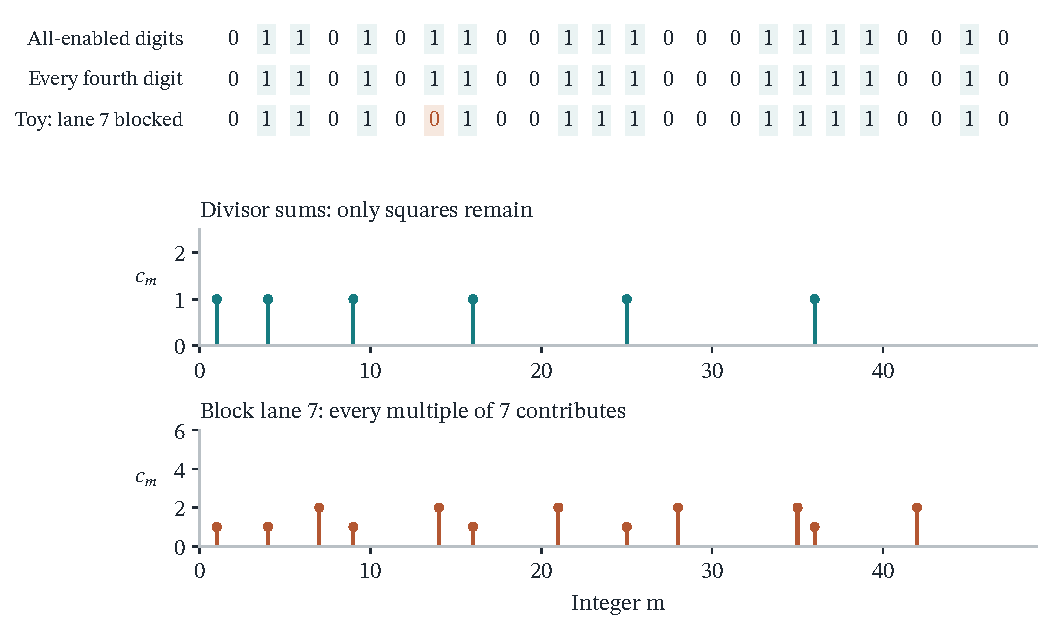
\includegraphics[width=.96\linewidth]{figures/01_digits_and_divisors.pdf}
\caption{Exact finite digit and divisor readings. The all-enabled mask is compared with an artificial mask that disables the lane of 7. The actual Goldbach question assigned to that lane is already settled by $10=5+5$. The lower plot illustrates how a failed lane would add a harmonic subseries.}
\label{fig:divisors}
\end{figure}

\subsection{A dimension change and a broken symmetry}

Exponentially damping the same divisor sums gives, for $t>0$,
\begin{equation}
 \Theta_{\Gold}(t)=1+2\sum_{m\ge1}c_me^{-\pi mt}
 =\theta(t)+4\sum_{n\ge1}\frac{b_n}{e^{\pi nt}-1},
 \qquad
 \theta(t)=\sum_{k\in\mathbb Z}e^{-\pi k^2t}.
 \label{fnd:heat-decomposition}
\end{equation}
Absolute convergence follows, for example, from
$0\le c_m\le\sum_{d\mid m}1$; the second equality follows by
summing over multiples.  It is legitimate to view $\Theta_{\Gold}$ as
the heat trace of a diagonal operator: there is one zero state and
energy $\pi m$ has multiplicity $2c_m$ whenever $c_m>0$.

\begin{proposition}[Heat-growth dimension]\label{fnd:dimension}
The limit
\[
 d_{\Gold}=2\lim_{t\downarrow0}\frac{\log\Theta_{\Gold}(t)}{\log(1/t)}
\]
exists, and equals one if Goldbach holds and two otherwise.
More precisely, in the latter case,
\begin{equation}
 \Theta_{\Gold}(t)\sim\frac{2S_g}{\pi t}\log\frac1t.
 \label{fnd:heat-leading}
\end{equation}
\end{proposition}
\begin{proof}
Under Goldbach, $\Theta_{\Gold}=\theta$, and Jacobi's transformation
$\theta(t)=t^{-1/2}\theta(1/t)$ gives
$\theta(t)\sim t^{-1/2}$; see \cite[20.7.32]{fndDLMF}.
If a lane $p$ fails, its single term in
\eqref{fnd:heat-decomposition} gives a lower bound of order
$t^{-1}$.  Since $b_n\le1$, splitting the remaining sum at
$n=1/t$ gives an upper bound $O(t^{-1}\log(1/t))$.
These estimates prove the dimension dichotomy without a density
theorem.

For the sharper equivalent, Theorem~\ref{fnd:balance} applied
lane by lane gives $\sum_{n\le y}b_n=(S_g/2)y+o(y)$.
Partial summation yields
$\sum_{n\le y}b_n/n=(S_g/2)\log y+o(\log y)$.
Consequently
\[
 \sum_{m\le y}c_m=\lfloor\sqrt y\rfloor+
 2\sum_{n\le y}b_n\lfloor y/n\rfloor
 \sim S_gy\log y,
\]
the floor error being $O(y)$.  Integrating this counting function
against $\pi t e^{-\pi ty}$ proves \eqref{fnd:heat-leading}.
Domination follows from $\sum_{m\le y}c_m=O(y\log(y+2))$.
\end{proof}

The word dimension here means the heat-growth exponent just defined.
Under Goldbach the operator agrees with the Laplacian spectrum of a
circle of circumference $2\sqrt\pi$.  The extra logarithm in
\eqref{fnd:heat-leading} is retained explicitly; no ordinary smooth
two-dimensional surface is being asserted in the other case.

\begin{proposition}[A single inversion identity]\label{fnd:inversion}
For every fixed $t>1$,
\[
 t^{-1/2}\Theta_{\Gold}(1/t)-\Theta_{\Gold}(t)\ge0,
\]
and equality holds if and only if Goldbach holds.
\end{proposition}
\begin{proof}
Jacobi's identity cancels the two theta terms in
\eqref{fnd:heat-decomposition}.  What remains is
\[
 4\sum_{n\ge1}b_n\left[
 \frac{t^{-1/2}}{e^{\pi n/t}-1}
 -\frac1{e^{\pi nt}-1}\right].
\]
Every bracket is positive.  In fact, for $u=\pi n/t$,
convexity gives $e^{t^2u}-1\ge t^2(e^u-1)$, while
$t^{-1/2}>t^{-2}$.  Thus equality forces all $b_n$ to vanish;
a failed prime lane would have $b_p=1$.
\end{proof}

The same transform can locate the first failure, if one exists.
Put $E_{\Gold}(t)=\Theta_{\Gold}(t)-\theta(t)$.  If $p_*$ is the smallest
failed-lane prime, its first nonzero exponential coefficient is four:
\begin{equation}
 E_{\Gold}(t)=4e^{-\pi p_*t}\bigl(1+O(e^{-\pi t})\bigr)
 \quad(t\to\infty),\qquad
 p_*=-\frac1\pi\lim_{t\to\infty}\frac{\log E_{\Gold}(t)}t.
 \label{fnd:first-heat-failure}
\end{equation}
To justify the error, divide the series in
\eqref{fnd:positive-divisors} by its first exponential term and
bound its remaining coefficients by the divisor function.  The
resulting tail is $O(e^{-\pi t})$ for $t\ge1$.
Moreover $-E_{\Gold}'(t)/E_{\Gold}(t)$ decreases to $\pi p_*$: its derivative
is minus the variance of the energies under their exponentially
weighted positive coefficients.  There are at least two energies,
$\pi p_*$ and $2\pi p_*$, so the decrease is strict.

\subsection{A finite exception list in a heat coefficient}

If there are finitely many disabled lanes, a further exact reading
is available.  Let $F=\{j:g_j=0\}$ be finite, and set
\[
 A(s)=\sum_{j\in F}p_j^{-s}\prod_{r<j}(1-p_r^{-s}),\qquad
 C(s)=\sum_{j\in F}p_j^{-s}\prod_{r<j}(1+p_r^{-s}),\qquad
 B=\sum_{j\in F}2^{j-1}.
\]
Here $B$ is the integer whose binary digits list the disabled lanes.
These are finite Dirichlet polynomials, and $A(1)=S_g$.

\begin{proposition}\label{fnd:heat-binary}
For a finite failed-lane set in the Goldbach construction,
\begin{align}
 \Theta_{\Gold}(t)={}&\frac2{\pi t}
 \left[S_g\log(1/t)+(\gamma-\log\pi)S_g+A'(1)\right]
 \notag\\
 &+\frac{1+C(1/2)}{\sqrt t}-B+O_F(\sqrt t)
 \qquad(t\downarrow0).
 \label{fnd:heat-binary-expansion}
\end{align}
Thus the constant term after the three divergent terms have been
removed records the entire finite exception list in binary.
\end{proposition}
The mechanism is a residue calculation: the growing terms come from the
poles at 1 and $1/2$, while the constant term comes from the pole of the
gamma factor at zero. The cancellation at that last pole leaves a sum of
distinct powers of two. The full calculation is in
Appendix~\ref{app:fnd:heat-binary}.

For example, an artificial message that disables lanes with indices
$2$ and $4$ has remaining constant term $-(2+8)=-10$. Read the magnitude
as binary $1010$: the two ones recover those exact indices. The actual
Goldbach questions attached to these lanes, $6$ and $10$, have known
representations; the example illustrates the encoding for a general mask.
The limiting growth detects that something was removed. Its finite part
can remember exactly what was removed.

The finiteness hypothesis belongs to this last proposition.  The
Basel alternative, the dimension dichotomy, and the first-failure
reading required no such assumption.  Each was obtained from the
same nonnegative divisor sums, so a single construction supplies
several different levels of information.

\IfFileExists{sections/sampling.tex}{\section{A staircase made by sampling the digits}
\label{samp:section}

Reading the digits at equally spaced positions gives another real number:
\[
 Y_g(a,d)=\sum_{j\ge0}x_g(a+jd)2^{-j-1}.
\]
Now choose the starting point $a$ and the step $d$ uniformly from
$1,\ldots,N$, subject to $\gcd(a,d)=1$.  This last restriction prevents
the entire progression from being trapped in a common prime lane.
Let $\nu_{g,N}$ be the distribution of $Y_g(a,d)$.  Its limiting
distribution gives a curve that rises across every interval, even in
examples where its derivative is zero almost everywhere.  The apparent
contradiction disappears once we distinguish total rise from the slope
at a typical point.

Write $\mathcal F=\{p_j:g_j=0\}$ for the disabled primes.  The hypothesis
needed below says that the successful primes retain a divergent
reciprocal sum:
\begin{equation}
 \sum_{p\notin\mathcal F}\frac1p=\infty.
 \label{samp:success-hypothesis}
\end{equation}
It holds unconditionally for the actual Goldbach mask.  Indeed, let
$E(Y)$ count even Goldbach exceptions in $[4,Y]$ and let
$A(R)=\#(\mathcal F\cap[2,R])$.  Pintz's Theorem~1
\cite{sampPintz2018} states that $E(Y)<Y^{18/25}$ beyond an
ineffective threshold.  The prime number theorem therefore gives
\begin{equation}
 A(R)=E\bigl(2(\pi(R)+1)\bigr)
 \ll (R/\log R)^{18/25} \quad(R\ge3).
 \label{samp:pintz}
\end{equation}
Partial summation shows $\sum_{p\in\mathcal F}1/p<\infty$, whereas
the sum over all primes diverges.  We use this established estimate
as an input.  Its precise exponent is useful later; here any power
strictly smaller than one would suffice.

\begin{theorem}[Primitive sampling]\label{samp:staircase}
Assume \eqref{samp:success-hypothesis}.  Then $\nu_{g,N}$ converges
weakly to a nonatomic probability measure $\nu_g$ of full support
$[0,1]$ and Hausdorff dimension one.  Its Lebesgue decomposition is
\begin{equation}
 \nu_g=L_g\,\mathrm{Leb}+\nu_{g,\mathrm{sc}},\qquad
 L_g=\prod_{p\in\mathcal F}\frac1{p+1},
 \label{samp:decomposition}
\end{equation}
where $\nu_{g,\mathrm{sc}}$ is singular continuous.  The empty product
is one; an infinite product here is zero.  Consequently
\[
 G_g(y):=\nu_g([0,y])\quad(0\le y\le1)
\]
is a homeomorphism of $[0,1]$ onto itself and
$G_g'(y)=L_g$ for Lebesgue-almost every $y$.
\end{theorem}

Full support means that every nonempty open interval receives positive
probability.  Singular means that a set of ordinary length zero carries
the measure.  Dimension one means that every set carrying its full mass
has Hausdorff dimension one.  These properties can coexist: small in
length need not mean small in dimension.  We do not claim that the
measure has the same local dimension at almost every point.

The mechanism is easier to see than the full convergence proof.
Choose, independently at every prime $p$, a residue pair $(U,V)\bmod p$
uniformly among the $p^2-1$ pairs other than $(0,0)$.  These simultaneous
residues are a primitive profinite pair.  Independently choose fair
bits $B_0,B_1,\ldots$.  The limiting sampled real has the law of
\[
 Z_g=\sum_{j\ge0}\bigl(1-h_g(U+jV)\bigr)B_j2^{-j-1}.
\]
Thus an open lane contributes a fair bit and a disabled lane contributes
zero.  This is a theorem about the average over starting points and
steps; it does not assume that the original consecutive digits are
independent.

A lane $p$ is visited precisely when $p$ does not divide $V$.  The
probability that it is avoided is $1/(p+1)$.  Consequently every bit is
free precisely on an event of probability $L_g$; that event supplies the
uniform part of the measure.  Once a disabled lane is visited, zeros
repeat on an infinite arithmetic progression.  Such digit strings form
a single Lebesgue-null set, which carries the remaining part.

This explains the decomposition and its product formula.  Full support
comes from making any finite prefix open by finitely many compatible
congruences.  Full dimension requires an additional limiting argument:
there are positive portions of the law with a proportion of free bits
arbitrarily close to one.  The complete proof, including the
Frantzikinakis--Host variable-step cancellation that produces the fair
bits, is in Appendix~\ref{samp:proofs}.


\begin{corollary}\label{samp:goldbach-trichotomy}
For the original Goldbach constant, $G_{\Gold}$ is the identity if and
only if Goldbach holds.  If there are finitely many exceptions and at least one, then
\[
 G_{\Gold}'(y)=\frac1{\prod_{p\in\mathcal F}(p+1)}\in(0,1)
 \quad\hbox{almost everywhere}.
\]
There are infinitely many Goldbach exceptions if and only if
$G_{\Gold}'=0$ almost everywhere.  In this last case $G_{\Gold}$ is a singular
homeomorphism whose associated measure has dimension one.
\end{corollary}

This phenomenon also has an unconditional explicit example.  Disable
exactly the lanes
\begin{equation}
 \mathcal F_* =\{p_{2^j}:j\ge2\}.
 \label{samp:explicit-mask}
\end{equation}
This is a concrete mask, defined without asking any unresolved arithmetic
question.  Its disabled-prime reciprocal sum converges because $p_{2^j}>2^j$.  The associated
$G_*$ is therefore a strictly increasing singular homeomorphism,
with full-support measure of dimension one.  Thus the geometry
exists independently of which Goldbach alternatives occur.
}{}

\section{Reading several digits at coprime positions}
\label{fnd:correlations}

The divisor reading led to a positive spectrum.  We now try a different
experiment: select several digit positions, insisting that no two have
a common prime factor.  This prevents two positions from drawing their
least prime from the same lane.  Consequently a correlation of $k$
digits can ask whether there are at least $k$ disabled lanes.

For independent uniform integers $n_1,\ldots,n_k$ in $[1,N]$, let
$\mathcal C_{k,N}$ be the event that they are pairwise coprime.
Define $M_0(g)=1$ and, for $k\ge1$,
\begin{equation}
 M_k(g)=\lim_{N\to\infty}
 \E\left[\prod_{i=1}^k a_g(n_i)\,\middle|\,\mathcal C_{k,N}\right].
 \label{fnd:marked-moments}
\end{equation}
We will prove that this limit exists.  Throughout this section an
arbitrary binary mask is allowed, including $g_1=0$.

At one prime $p$, pairwise coprimality permits either no divisible
coordinate or exactly one.  Their total probability is
$(1-1/p)^k+k p^{-1}(1-1/p)^{k-1}$.  It follows that
\begin{equation}
 K(k)=\lim_{N\to\infty}\Prob(\mathcal C_{k,N})
 =\prod_p(1-p^{-1})^k\left(1+\frac{k}{p-1}\right)>0.
 \label{fnd:coprime-kernel}
\end{equation}
To justify the infinite product, first impose the restrictions only at
primes at most $R$ and use the Chinese remainder theorem.  The probability
of a collision at a larger prime is at most
$\binom{k}{2}\sum_{p>R}p^{-2}$, uniformly in $N$.
This tends to zero, and the local factors differ from one by
$O_k(p^{-2})$.  In particular $K(0)=K(1)=1$ and
$K(2)=1/\zeta(2)=6/\pi^2$.

The Euler product in \eqref{fnd:coprime-kernel} is classical.  Written
as
$\prod_p(1-1/p)^{s-1}(1+(s-1)/p)$, it is the arithmetic factor
appearing in mod-Poisson descriptions of the number of distinct prime
divisors; see \cite[Section 4]{fndKowalskiNikeghbali2009}.
Here its role is dictated by the coprimality experiment itself.

\begin{proposition}[Correlations count available lanes]
\label{fnd:moment-positivity}
The limits in \eqref{fnd:marked-moments} exist and satisfy
\begin{equation}
 0\le M_k(g)\le1,\qquad M_1(g)=S_g,\qquad
 M_k(g)>0\ \Longleftrightarrow\ \#\{j:g_j=0\}\ge k.
 \label{fnd:moment-tests}
\end{equation}
They have the following probability description.  Independently at
each prime $p$, choose one of $k$ coordinates with probability
$1/(p+k-1)$ each, or choose none with probability
$(p-1)/(p+k-1)$.  A coordinate is labelled by the first prime that
chooses it.  Then $M_k(g)$ is the probability that all $k$ labels
belong to disabled lanes.
\end{proposition}
Each factor $a_g(n_i)$ is a sign, so its product can be negative.
Yet the limit is a probability. Averaging cancels the Liouville oscillation
on every enabled lane; the disabled lanes leave a persistent contribution.
Coprimality forces the first prime labels to be distinct. Those two facts
explain both the nonnegativity and the exact counting test. The truncation
argument that justifies them is in Appendix~\ref{app:correlations}.


We collect the correlations into two entire functions,
\begin{equation}
 \Phi_g(z)=\sum_{k\ge0}M_k(g)\frac{z^k}{k!},\qquad
 \Psi_g(z)=\sum_{k\ge0}K(k)M_k(g)\frac{z^k}{k!}.
 \label{fnd:two-functions}
\end{equation}
Both series converge absolutely everywhere, with modulus at most
$e^{|z|}$.  The first averages after conditioning on coprimality;
the second gives noncoprime tuples score zero and averages over
all tuples.  If there are exactly $r$ disabled lanes, each function
is a polynomial of degree $r$.  Under Goldbach both are identically
one.  When there are infinitely many disabled lanes, every
coefficient is positive.

\subsection{A positive operator behind the correlations}

The change from conditional to unconditional averages has a strong
spectral effect.  Its proof also gives an explicit construction.
A positive operator is a matrix with a nonnegative quadratic form,
possibly on an infinite-dimensional space. Its eigenvalues are nonnegative.
In the theorem below they also have a finite sum. Such an operator has a
determinant $\prod_j(1+\alpha_j z)$, so its zeros can lie only on the
negative real axis. The assertion is that the unconditional correlation
function has precisely this structure. Write $\mathcal F=\{p_j:g_j=0\}$
for its disabled primes.

\begin{theorem}[The positive mask operator]\label{fnd:mask-operator}
For every prime mask there is a positive trace-class operator $A_g$
with
\begin{equation}
 \Psi_g(z)=\det(I+zA_g),\qquad
 \operatorname{tr}A_g=S_g,\qquad
 \operatorname{rank}A_g=\#\mathcal F.
 \label{fnd:positive-determinant}
\end{equation}
The rank may be infinite.  Every zero of $\Psi_g$ is negative and real.
\end{theorem}
The construction processes primes one at a time. Each disabled lane
adds one positive spectral direction, while the trace records the total
disabled-lane density. Appendix~\ref{app:fnd:mask-operator} gives the
explicit differential recurrence and the limiting operator.

This explains the rank statement in ordinary terms: counting the
operator's nonzero directions counts the missing answers. If exactly
three lanes are disabled, the infinite construction produces only three
such directions.

The proof establishes a summable spectrum for every mask, without
requiring any estimate for Goldbach's exceptional set.  It also gives
the useful bound
\begin{equation}
 K(k)M_k(g)\le S_g^k.
 \label{fnd:moment-bound}
\end{equation}
Indeed, $K(k)M_k(g)/k!$ is the $k$th elementary symmetric function
of the $\alpha_j$, and the distinct-index terms in
$(\sum_j\alpha_j)^k$ contribute exactly $K(k)M_k(g)$.

\subsection{Two missing lanes, two geometries of zeros}

The distinction between the two correlation functions becomes visible
in a small example. Artificially disable just the lanes of $3$ and $5$.
Their densities add to $1/6+1/15=7/30$. Two coprime positions can use
those two lanes in either order; the prime-assignment model gives
$M_2=2(1/3)(1/4)(1/6)=1/36$. Consequently
\[
 \Phi_g(z)=1+\frac7{30}z+\frac1{72}z^2,
 \qquad
 \Psi_g(z)=1+\frac7{30}z+\frac1{12\pi^2}z^2.
\]
The discriminant of the first polynomial is $-1/900$, so its two zeros
are nonreal. The second has two negative real zeros, as the operator
theorem requires. The same two disabled lanes have produced both
geometries. Conditioning on coprimality changes the zeros, even though
both functions retain the exact count of missing lanes.

\begin{figure}[htbp]
\centering
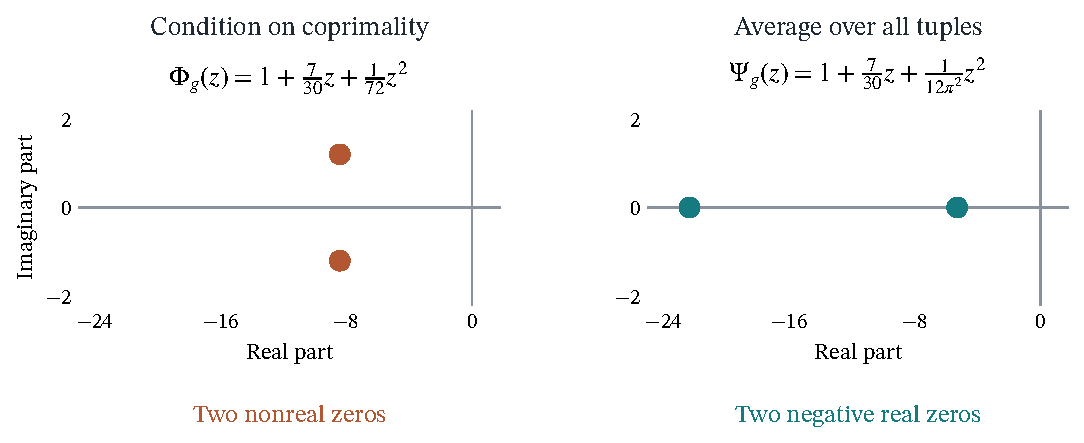
\includegraphics[width=.96\linewidth]{figures/05_two_averages.pdf}
\caption{The same artificial message disables the lanes of 3 and 5.
Conditioned and unconditioned correlations give two quadratic polynomials
with different zero locations. The coefficients are exact; coordinates
in the plot are their numerical root locations.}
\label{fig:two-averages}
\end{figure}

This is the question that will lead to the curve: can we describe that
change of average by introducing an independent random scale?

\IfFileExists{sections/phi_growth.tex}{\subsection{What the growth and zeros count}
\label{grw:section}

The operator behind $\Psi_g$ controls the location of its zeros.
The companion $\Phi_g$ records how quickly disabled lanes accumulate.
If those primes grow sparse, the function grows slowly; if they grow
more numerous, it grows faster.  For the Goldbach member this comparison
also turns the conjecture into a statement about complex zeros.

Put $a_k=M_k(g)/k!$ and $B_g(R)=\#(\mathcal F\cap[2,R])$.
If all $k$ labels in the prime-assignment model of
Proposition~\ref{fnd:moment-positivity} are masked, their first
assigned primes are $k$ distinct members of $\mathcal F$.
For a chosen set of $k$ primes, sum over its $k!$ assignments to the
labels and discard the first-assignment restrictions.  Independence
between primes gives the useful bound
\begin{equation}
 a_k\le e_k\left(\frac1{p+k-1}:p\in\mathcal F\right)
 \le e_k\left(\frac1p:p\in\mathcal F\right),
 \label{grw:coefficient-majorant}
\end{equation}
Here $e_k$ means the sum of products over all $k$-element subsets; for
example $e_2(w)=\sum_{p<q}w_pw_q$.  Thus, when
$\sum_{p\in\mathcal F}1/p<\infty$,
\begin{equation}
 |\Phi_g(z)|\le\Phi_g(|z|)
 \le P_{\mathcal F}(|z|):=
       \prod_{p\in\mathcal F}(1+|z|/p).
 \label{grw:majorant}
\end{equation}
The product bounds the function from above.  Its factors are not being
identified with the zeros of $\Phi_g$.

The \emph{order} of an entire function records the power in its
exponential growth: roughly, growth like $\exp(r^\alpha)$ on disks of
radius $r$ gives order $\alpha$.  The following theorem matches that
analytic exponent with a counting exponent for the disabled primes.

\begin{theorem}[Counting exponent and entire-function order]
\label{grw:order}
Suppose the disabled-prime counting exponent
\[
 \eta_g=\limsup_{R\to\infty}
 \frac{\log\max(1,B_g(R))}{\log R}
\]
is strictly less than one.  Then $\Phi_g$ has order exactly $\eta_g$.
Formally the order is the limsup of $\log\log \max_{|z|\le r}|\Phi_g(z)|$
divided by $\log r$; constants and polynomials have order zero by convention.  For the actual
Goldbach mask,
\begin{equation}
 \operatorname{ord}\Phi_{\Gold}
 =\limsup_{Y\to\infty}\frac{\log\max(1,E(Y))}{\log Y}
 \le\frac{18}{25},
 \label{grw:goldbach-order}
\end{equation}
and, as $r\to\infty$,
\begin{equation}
 \log\max_{|z|\le r}|\Phi_{\Gold}(z)|
 =\log\Phi_{\Gold}(r)\ll(r/\log r)^{18/25}.
 \label{grw:quantitative-growth}
\end{equation}
In particular, for an absolute constant $C$ and $k\ge2$,
\begin{equation}
 M_k(\Gold)\le
 \left(\frac{C}{k^{7/18}\log(k+1)}\right)^k.
 \label{grw:moment-bound}
\end{equation}
\end{theorem}
The proof is in Appendix~\ref{grw:proofs}.  Its two estimates have
opposite roles.  Summing over every possible set of disabled primes
bounds the function from above.  Requiring the first $k$ disabled
primes to hit distinct labels supplies a matching lower bound on its
order.  The analytic exponent therefore cannot lose the arithmetic
counting exponent.


\begin{corollary}[Zeros count the exceptions]\label{grw:zeros}
Under the hypothesis of Theorem~\ref{grw:order}, list the zeros
of $\Phi_g$ with multiplicity as $(\zeta_j)$.  Then
\begin{equation}
 \Phi_g(z)=\prod_j(1-z/\zeta_j),\qquad
 \sum_j|\zeta_j|^{-1}<\infty,\qquad
 \sum_j\zeta_j^{-1}=-S_g.
 \label{grw:factorization}
\end{equation}
Counting multiplicity, the number of zeros equals the number of
disabled lanes, allowing infinity.
If $n_g(R)$ counts the zeros in $|z|\le R$, with multiplicity, then
\begin{equation}
 \limsup_{R\to\infty}
 \frac{\log\max(1,n_g(R))}{\log R}=\eta_g.
 \label{grw:zero-exponent}
\end{equation}
For the actual Goldbach function,
\[
 \GC\ \Longleftrightarrow\ \Phi_{\Gold}\text{ has no complex zeros},
 \qquad n_{\Gold}(R)\ll(R/\log R)^{18/25}.
\]
If there are infinitely many exceptions, every complex value is
attained by $\Phi_{\Gold}$ infinitely often.
\end{corollary}
\begin{proof}
Hadamard's factorization theorem \cite{sampHadamard1893} says that
an entire function of order less than one has a genus-zero product
and a constant exponential prefactor.  Since $\Phi_g(0)=1$, this
gives the first two assertions of \eqref{grw:factorization};
differentiation at zero gives its last assertion because
$\Phi_g'(0)=M_1(g)=S_g$.  For a finite mask the polynomial degree
is $\#\mathcal F$.  For an infinite mask all coefficients are
positive, so the function is not a polynomial; the factorization
then forces infinitely many zeros.  The same argument applied to
$\Phi_g-w$ shows infinite attainment of each $w\in\mathbb C$
when the mask is infinite.

Jensen's formula and $\Phi_g(0)=1$ give
$n_g(R)\log2\le\log\Phi_g(2R)$, which bounds the zero-counting
exponent by $\eta_g$ and gives the displayed quantitative estimate.
Conversely, if that exponent were $\lambda<\eta_g$, choose
$\lambda<\beta<\eta_g<1$.  The product
\eqref{grw:factorization}, together with
$n_g(t)\ll_\beta t^\beta$, implies
\[
 \log\max_{|z|\le r}|\Phi_g(z)|
 \le\sum_j\log(1+r/|\zeta_j|)=O_\beta(r^\beta)
\]
by the same integration used in \eqref{grw:stieltjes}, starting
below the smallest zero modulus.  This contradicts its order.
The zero-order case follows from the upper bound and nonnegativity.
\end{proof}

These are zeros of the mask function.  The worked example above shows
that they can be nonreal.  The sparsity hypothesis is essential to the
factorization argument.
Also, order zero alone does not mean finitely many exceptions: an
infinite mask with subpower counting function has the same order.
The improved moment estimate measures a statistic of our
construction; it does not improve the imported bound for $E(Y)$.

\subsection{One bias can hide infinitely many changes}
\label{grw:collision-section}

There is a sharp reason to keep the higher correlations rather
than only the proportion of zero digits.  Put
$\delta_p=p^{-1}\prod_{q<p}(1-1/q)$, so
$S_g=\sum_{p\in\mathcal F}\delta_p$.

\begin{proposition}\label{grw:bias-collision}
Among masks known to have finitely many disabled lanes, the exact bias $S_g$ determines the mask.
Nevertheless, for every sufficiently large prime $p$, there is an
infinite set $\mathcal H=\{q_1<q_2<\cdots\}$ of primes greater than
$p$ such that
\begin{equation}
 \sum_{q\in\mathcal H}\delta_q=\delta_p,\qquad
 q_{j+1}/q_j\longrightarrow\infty,
 \qquad \#(\mathcal H\cap[2,R])=o(\log R).
 \label{grw:collision}
\end{equation}
Thus two masks can have exactly the same digit bias while one has
one disabled lane and the other has infinitely many.
\end{proposition}
\begin{proof}
If $P$ is the largest prime of a finite nonempty mask, then
$\delta_P$ has $P$-adic valuation $-1$: its numerator contains only
factors $q-1<P$, and its denominator is the primorial through $P$.
Every earlier $\delta_q$ has nonnegative $P$-adic valuation.
Consequently $P$ is the largest prime dividing the reduced
denominator of $S_g$.  Recover $P$, subtract $\delta_P$, and repeat.

List all primes as $p_i$ and set $d_i=\delta_{p_i}$.  These weights
decrease strictly to zero and
\[
 d_i/d_{i+1}=p_{i+1}/(p_i-1)\longrightarrow1
\]
by the prime number theorem.  Choose $p$ beyond a point where every
consecutive ratio is less than two.  Starting with residual
$r_0=\delta_p$, repeatedly subtract the largest weight at a prime
greater than $p$ which does not exceed the residual.
The first choice is the successor of $p$.  If $q$ is a later
choice and $q^-$ its immediate prime predecessor, the residual
after subtraction satisfies
\[
 0\le r_{\mathrm{new}}
 \le\delta_{q^-}-\delta_q=o(\delta_q).
\]
The ratio bound makes $r_{\mathrm{new}}<\delta_q$, so no weight is
used twice and selected primes strictly increase.  The process
cannot terminate: a finite sum at primes greater than $p$ has a
reduced denominator containing its largest prime, unlike
$\delta_p$.  It therefore makes infinitely many selections, and
$r_j<\delta_{q_j}\to0$ proves the sum identity.

The next selected weight is at most the preceding residual, hence
$\delta_{q_{j+1}}/\delta_{q_j}\to0$.  Mertens' product estimate
$\delta_q\sim e^{-\gamma}/(q\log q)$ forces
$q_{j+1}/q_j\to\infty$.  For any fixed $C>1$, these ratios
eventually exceed $C$, so the counting function is at most
$\log R/\log C+O_C(1)$.  Letting $C$ tend to infinity proves
\eqref{grw:collision}.
\end{proof}

The equality is exact, so it survives arbitrarily accurate measurement
of the digit frequency.  For these two masks $\Phi_g'(0)$ agrees,
but their functions are
respectively linear and transcendental entire.  The second has
order zero and infinitely many zeros by the preceding results.
This is an example within the mask family; it asserts no actual
Goldbach exception, and no collision between the whole functions.
}{}

\section{The curve selected by coprimality}
\label{fnd:curve-section}

The positive operator belongs to a particular message.  The factor
$K(k)$ that connected its determinant with the original correlations
does not.  We now isolate that universal factor.  Define
\begin{equation}
 K(s)=\prod_p(1-p^{-1})^s\left(1+\frac{s}{p-1}\right),
 \qquad s\in\mathbb C,
 \label{fnd:entire-k}
\end{equation}
using the real logarithm of $1-1/p$.  The local factor is
$1+O_B(p^{-2})$ on $|s|\le B$, so the product is entire.
Its zeros are simple and occur precisely at $s=1-p$:
away from these points the logarithm of the tail converges
absolutely, and at each such point exactly one factor vanishes.

The reciprocals of its nonnegative integer values are moments of a
positive random variable.  This kind of reciprocal-Mellin construction,
including its role in cancelling arithmetic factors by an auxiliary
random scale, occurs in Barhoumi--Andr\'eani's dissertation
\cite[Section 3.6.1]{fndBarhoumi2013}.  Its general mechanism is
therefore prior work.  Our aim here is the concrete coprimality law
and its actual density.

\begin{proposition}[The universal scale]\label{fnd:prime-noise}
Let $(U_p)_p$ be independent uniform variables on $(0,1)$.  The product
\begin{equation}
 W=\prod_p\frac p{p-1}U_p^{1/(p-1)}
 \label{fnd:w-product}
\end{equation}
converges almost surely to a finite positive random variable, and
\begin{equation}
 \E W^s=\frac1{K(s)}\qquad(\Re s>-1).
 \label{fnd:mellin}
\end{equation}
This is the exact half-plane of finite absolute moments.  In particular,
$\E W=1$ and $\Var W=\pi^2/6-1$.
\end{proposition}
\begin{proof}
Write $E_p=-\log U_p$, so the $E_p$ are independent exponentials
of mean one.  The logarithm of the $p$th factor is
$\log(p/(p-1))-E_p/(p-1)$.  Its mean is $O(p^{-2})$
and its variance is $(p-1)^{-2}$.  The centered independent series
converges almost surely and in $L^2$, while its means sum absolutely.
Exponentiation proves the product assertion.

For a finite prime cutoff $R$, direct integration gives
$\E W_R^s=1/K_R(s)$ for $\Re s>-1$.  If $\sigma=\Re s$,
choose $r>1$ with $r\sigma>-1$; this is always possible.
The product of moments $\E W_R^{r\sigma}$ is uniformly bounded,
since its local factors are $1+O_{s,r}(p^{-2})$.
Thus $(W_R^s)_R$ is uniformly integrable, and almost-sure
convergence proves \eqref{fnd:mellin}.
For $\sigma\le-1$, write $W=2U_2V$ with $V>0$ independent
of $U_2$.  Conditional integration over $U_2$ makes
$\E W^\sigma$ infinite.  Finally $K(1)=1$ and
$K(2)=6/\pi^2$ give the stated mean and variance.
\end{proof}

In terms of the cited general construction, the logarithm of $W$ is
a deterministic constant plus
$\sum_p (1-E_p)/(p-1)$.  This identifies the specialization directly.
The same scale now reverses the coprimality weighting of every message.

\begin{corollary}[The exact bridge]\label{fnd:bridge}
For every mask and every $z\in\mathbb C$,
\begin{equation}
 \Phi_g(z)=\E\Psi_g(zW)=\E\det(I+zWA_g).
 \label{fnd:bridge-equation}
\end{equation}
\end{corollary}
\begin{proof}
All coefficients of $\Psi_g$ are nonnegative.  Tonelli and
\eqref{fnd:mellin} give
\[
 \E\Psi_g(|z|W)=
 \sum_{k\ge0}K(k)M_k(g)\frac{|z|^k}{k!}\E W^k
 =\Phi_g(|z|)\le e^{|z|}.
\]
Absolute integrability therefore permits the same termwise exchange
for complex $z$, proving the identity.
\end{proof}

We have reached a division of roles.  The operator carries the
message; $W$ carries the universal effect of changing the average.
It is this universal law that produces the curve in the title.

\subsection{The entire density theorem}

A probability density is initially a real function, defined on the
possible values of its random variable.  The density here has an
additional analytic structure: it continues to an entire function,
and the positions of its nonzero Taylor coefficients recover the
primes exactly.  Reciprocal transforms of real-zero entire products
have a classical theory, notably Schoenberg's
\cite{fndSchoenberg1947}; the following proof establishes this
specific density and the required convergence directly.

\begin{theorem}[The prime density]\label{fnd:entire-density}
The random variable $W$ has a density on $(0,\infty)$ which extends
to the entire function
\begin{equation}
 f(z)=\sum_{p\text{ prime}}\frac{z^{p-2}}{K'(1-p)}.
 \label{fnd:density-series}
\end{equation}
Consequently
\begin{equation}
 f^{(n)}(0)\ne0\quad\Longleftrightarrow\quad n+2\text{ is prime}.
 \label{fnd:prime-taylor-support}
\end{equation}
With $c_p=1/K'(1-p)$, the nonzero coefficients have signs
$\operatorname{sgn}(c_p)=(-1)^{\pi(p)-1}$ and satisfy
\begin{equation}
 \log|c_p|=-p\log\log p+O(p).
 \label{fnd:residue-decay}
\end{equation}
\end{theorem}

\paragraph{Why a probability density contains this pattern.}
With only finitely many primes, take logarithms of the defining random
product. We obtain a sum of independent exponential variables, whose
rates are $p-1$. Returning from logarithms turns these rates into powers
$z^{p-2}$ in a finite density formula. As the prime cutoff grows, the
right endpoint of that formula moves to infinity and its coefficients
converge. This is how the primes become derivative positions.

There are two things to prove: convergence of the entire series, and
identification of its restriction to the positive axis with the actual
probability density. Appendix~\ref{app:fnd:entire-density} proves both,
including the coefficient estimate in the theorem.

The support of the Taylor series begins
\[
 f(z)=c_2+c_3z+c_5z^3+c_7z^5+c_{11}z^9+c_{13}z^{11}+\cdots.
\]
The construction did not begin by writing down a prime-supported
series.  It began with coprimality probabilities, then produced a
positive random scale and finally its density.  The theorem says
that positivity, normalization, entire continuation and this exact
prime pattern coexist in the same curve.

Consider what the derivative test says at its first few positions.
The second derivative vanishes at zero because $2+2=4$ is composite.
The third derivative does not vanish because $3+2=5$ is prime. The
fourth vanishes, and the fifth does not. The test continues forever.
These are exact zeros amid exact nonzeros, rather than a tendency for
prime positions to have larger coefficients.

The source of the curve is equally important. An observer can describe
the sampling experiment and ask for the resulting probability density
before asking any question about its derivatives. The arithmetic pattern
then appears inside that density. This is what distinguishes the result
from merely choosing a list of coefficients indexed by primes.

\begin{figure}[htbp]
\centering
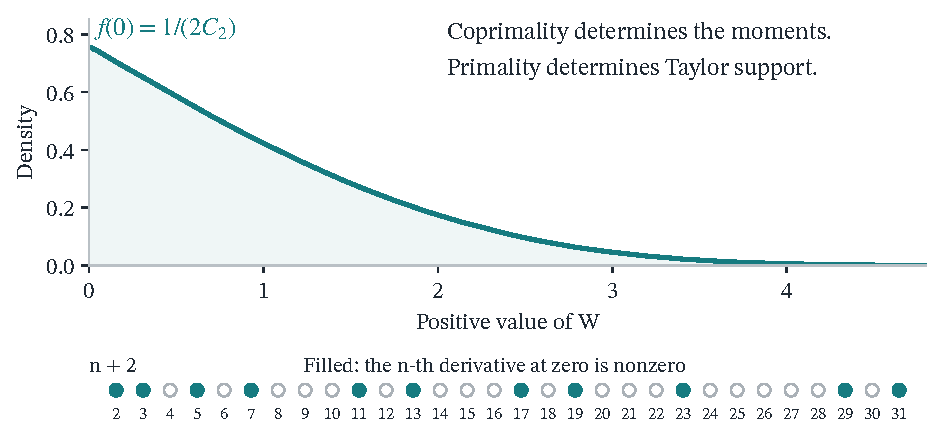
\includegraphics[width=.96\linewidth]{figures/02_prime_density.pdf}
\caption{The density on the positive axis and its exact Taylor-support pattern. The curve is an explicitly approximate conditional Monte Carlo preview with 180,000 samples, primes through 2,000 and seed 271828; no numerical error certificate is claimed. The marked derivative positions represent Theorem~\ref{fnd:entire-density}, not a numerical derivative test.}
\label{fig:density}
\end{figure}

\subsection{Reflection, a symmetric distribution, and the twin constant}

Let
\begin{equation}
 \mathfrak C_2=\prod_{p>2}\frac{p(p-2)}{(p-1)^2}
 \label{fnd:twin-constant}
\end{equation}
be the usual twin-prime constant.  Its appearance below uses only
this convergent product, with no assertion about twin-prime
infinitude.

\begin{corollary}\label{fnd:reflection}
The entire density satisfies
\begin{equation}
 f(0)=\frac1{2\mathfrak C_2},\qquad
 f(z)+f(-z)=\frac1{\mathfrak C_2}\quad(z\in\mathbb C).
 \label{fnd:reflection-identity}
\end{equation}
It is nonincreasing on the real line, with limits
$1/\mathfrak C_2$ and zero at negative and positive infinity,
respectively.  Consequently
\[
 \SymCDF(x)=\mathfrak C_2 f(-x)
\]
is a symmetric cumulative distribution function on $\mathbb R$.
The entire function $f$ is bounded on the real axis and has
infinite order in the complex plane.
\end{corollary}
\begin{proof}
Writing $W=2U_2V$ and conditioning on $V$ gives
\begin{equation}
 f(w)=\E\left[\frac1{2V}\mathbf1_{\{2V>w\}}\right],
 \qquad w>0.
 \label{fnd:density-monotone}
\end{equation}
The independent prime-$3$ factor makes the distribution of $V$
nonatomic.  Once its inverse moment below is finite, dominated
convergence makes the right-hand side continuous, so this identity
holds pointwise for the entire density, not merely almost everywhere.
The inverse moment of $V$ is
$\E V^{-1}=\prod_{p>2}(p-1)^2/[p(p-2)]=1/\mathfrak C_2$;
the moment passage follows as in Proposition~\ref{fnd:prime-noise},
now with domain $\Re s>-2$.  Thus
$f(0)=1/(2\mathfrak C_2)$ and $f$ is nonincreasing on the
positive half-line.  Integrability makes its limit there zero.
Every nonconstant exponent $p-2$ in
\eqref{fnd:density-series} is odd, proving the reflection identity.
This extends the monotonicity and gives the two endpoint limits,
from which the CDF assertion follows.

For completeness, the coefficient formula for the order of an
entire series is
$\rho=\limsup_{n\to\infty}n\log n/\log(1/|[z^n]f|)$,
with zero coefficients omitted.  Along $n=p-2$,
\eqref{fnd:residue-decay} makes this ratio asymptotic to
$\log p/\log\log p$, which tends to infinity.
\end{proof}

Thus a smooth bounded curve on the real line can have extremely
large growth in other complex directions.  For every fixed $a>0$, there are arbitrarily large $R$ for which
$\max_{|z|=R}|f(z)|>\exp(R^a)$, even though $f$ stays bounded on the
whole real axis. The prime pattern is
local analytic information at zero; ordinary plotting resolution
does not reveal its vanishing derivatives.  The reflection identity
provides a simple real counterpart of that analytic structure.

\subsection{Put the composites back}

The product defining $W$ uses only prime indices.  The missing
composite factors complete it to a familiar distribution.  On an
independent family of uniform variables define
\begin{equation}
 \Comp=\prod_{\substack{m\ge4\\m\text{ composite}}}
       \frac m{m-1}U_m^{1/(m-1)}.
 \label{fnd:composite-noise}
\end{equation}
Its logarithm converges by the same summable-mean and summable-variance
argument as before. We can now ask a simple question: what happens if
the prime contribution and the composite contribution are put back
together? The answer is the standard exponential distribution, whose
density is $e^{-w}$ for $w>0$.

\begin{proposition}[Prime--composite completion]\label{fnd:completion}
For independent $W$ and $\Comp$ defined above,
\begin{equation}
 W\Comp\ \overset{d}=\ \operatorname{Exp}(1),\qquad
 \E \Comp^s=\Gamma(1+s)K(s)\quad(\Re s>-1).
 \label{fnd:completion-law}
\end{equation}
\end{proposition}
\begin{proof}
Combine all integer factors up to $M$:
\[
 V_M=\prod_{m=2}^{M}\frac m{m-1}U_m^{1/(m-1)}.
\]
Its Mellin transform is
\[
 \E V_M^s=M^s\prod_{j=1}^{M-1}\frac j{j+s}
 =M^s\frac{\Gamma(M)\Gamma(1+s)}{\Gamma(M+s)}.
\]
This is also the Mellin transform of
$M\min(U_1,\ldots,U_{M-1})$, as follows directly by integrating
the density of the minimum.  Characteristic functions of the
logarithms identify the two laws.  For fixed $x\ge0$ and $M>x$,
the survival probability of the latter variable is
$(1-x/M)^{M-1}\to e^{-x}$.  Meanwhile $V_M$ converges almost
surely to the product $W\Comp$.  Thus $W\Comp$ is exponential.
Uniform integrability of fixed moments with real part greater
than $-1$ follows from a nearby moment exactly as in
Proposition~\ref{fnd:prime-noise}.  Independence and
\eqref{fnd:mellin} now give the second identity.
\end{proof}

This completion is a short specialization of classical beta and gamma
product identities.  It will also supply the composite random scale
in the later matrix construction.  The path from the constant to the
curve has therefore produced more than an encoding: the same
coprimality factor can change conditional averages, generate a
positive spectrum, and connect two complementary random products.

The second moments give a small numerical glimpse of this cancellation:
\[
 \E W^2=\frac{\pi^2}{6},\qquad
 \E \Comp^2=\frac{12}{\pi^2},\qquad
 \E(W\Comp)^2=2.
\]
The complete law, and not only this moment, becomes exponential.
The prime and composite factors separately retain their arithmetic
structure; their independent product reconstructs the distribution
obtained by allowing every integer factor.

\section{Two questions to ask the curve}\label{cq:section}

The density has already given us a way to recognize individual primes. It is
natural to ask whether familiar conjectures can be read from the probability
law without extracting its Taylor coefficients one at a time. Two observations
do this. One changes the way we sample the law and watches its variance. The
other compares two moments and watches the signs of a matrix's eigenvalues.

These are criteria: the relevant sign inequality and the unbounded matrix
index remain to be proved. Their interest is that the observables are ordinary
probabilistic and linear-algebraic objects belonging to the same law.

\subsection{The Riemann hypothesis as a variance comparison}

Write \(Y=\log W\). For \(t>-1\), change its distribution by giving an outcome
of size \(Y=y\) a weight proportional to \(e^{ty}\). More formally,
\[
 \E_t h(Y)=\frac{\E[W^t h(\log W)]}{\E W^t}.
\]
This is exponential tilting. Increasing \(t\) favors the larger values of
\(W\). If \(\kappa(t)=\log \E W^t=-\log K(t)\), differentiation gives
\begin{equation}\label{cq:variance}
 \Var_t(Y)=\kappa''(t)=\sum_p\frac{1}{(p-1+t)^2}.
\end{equation}
The variance is a softened count of primes. The prime number theorem suggests
replacing the prime atoms by the continuous density \(du/\log u\), giving
\[
 V_0(t)=\int_2^\infty\frac{du}{(u-1+t)^2\log u}.
\]
Does the actual variance eventually lie above or below this smooth comparison?

\begin{theorem}[An eventual variance deficit]\label{cq:rhvariance}
The Riemann hypothesis holds if and only if
\[
             \Var_t(\log W)<V_0(t)
             \qquad\text{for all sufficiently large }t.
\]
\end{theorem}

The word \emph{eventually} matters. This is an inequality along the positive
real axis, with no assumed simplicity or spacing of zeta zeros. Eventual-sign
criteria for RH have a long history; Robin's work \cite{Robin1984} is an
important example. The statistic here is the tilted variance of the law
already constructed.

\paragraph{What would an experimenter see?}
The parameter $t$ changes which outcomes matter most: increasing it
favors larger values of $W$. We then measure the spread of their
logarithms. The comparison curve $V_0(t)$ is obtained by replacing the
discrete primes with their smooth predicted density. The criterion
says that RH is exactly an eventual ordering of these two spreads.
No individual zero of zeta appears in the statement.

The proof exposes why a one-sided comparison is possible. Prime squares
give a negative correction to the smooth approximation. On RH, that
correction is larger than all the possible oscillations from the
nontrivial zeros combined. If RH fails, oscillations force crossings
in both directions arbitrarily far out. The complete argument and its
quantifiers are in Appendix~\ref{app:rh-variance}.

This is an exact reformulation attached to a probability law we already
met. Its usefulness as a route to RH would require a new way to compare
those variances. The theorem supplies the comparison to aim for.

\subsection{Twin primes hidden in matrices with positive entries}

For this observation we separate the prime \(2\), writing
\[
 W=2U_2V,\qquad
 K_o(s)=\prod_{p>2}(1-p^{-1})^s\left(1+\frac{s}{p-1}\right).
\]
Then \(\E V^s=1/K_o(s)\) for \(\Re s>-2\). Compare moments three units apart:
\[
 F(t)=\frac{\E V^t}{\E V^{t+3}}=\frac{K_o(t+3)}{K_o(t)},\qquad t>0.
\]
The number three has a purpose. Differences between odd primes are even;
a shift of three crosses precisely the gap of two before it reaches the next
possible gap.

For a symmetric matrix, its \emph{negative index} is the number of negative
eigenvalues, counted with multiplicity. Equivalently, it is the greatest
dimension of a subspace on which its quadratic form is strictly negative.

\begin{theorem}[A matrix count of twin pairs]\label{cq:twins}
Fix \(a>0\), and form
\[
 \mathsf H_N(a)=
 \left[\frac{(-1)^{i+j}F^{(i+j+2)}(a)}{(i+j+2)!}\right]_{0\leq i,j<N}.
\]
Every entry is strictly positive. Nevertheless,
\[
 \sup_{N\geq1}n_-(\mathsf H_N(a))
   =\#\{p>2:p\text{ and }p-2\text{ are prime}\}.
\]
Both sides are allowed to be infinite. The negative index is nondecreasing
in \(N\).
\end{theorem}

The surprise is the exact arithmetic count. A quotient of moments
of the probability law gives a sequence of positive-entry matrices whose
negative directions count twin pairs.

The general relation between signed moments and negative squares belongs to
indefinite moment theory \cite{BergChristensenMaserick1988}. We prove the
compact signed-measure step directly in the appendix, which also shows
exactly where the primes enter.

\paragraph{Why a negative direction means a twin pair.}
The moment quotient has one pole associated with each odd prime $p$.
Its residue is negative precisely when $p-2$ is also prime. This sign
test is elementary: the shift by three crosses the preceding odd prime
only when the two primes are twins.

The derivatives assemble those signed residues into a moment matrix.
Polynomials can separate any finite collection of its negative atoms,
turning each chosen twin pair into a negative direction in a sufficiently
large matrix. Conversely, the matrix cannot have more negative directions
than there are negative atoms. Appendix~\ref{app:twin-index} makes this
argument precise and controls the infinite tail.

Thus the matrices provide a counter whose reading can rise as their size
increases. The twin-prime conjecture says that this counter never reaches
a final value. All its entries are positive throughout; the signs being
counted belong to quadratic forms, which combine entries using both
positive and negative weights.

For comparison, the positive-entry matrix
$\left[\begin{smallmatrix}1&2\\2&1\end{smallmatrix}\right]$
has quadratic form $-2$ at the vector $(1,-1)$, and therefore one
negative direction. Our matrices turn this familiar linear-algebraic
possibility into an exact count of prime pairs.

\subsection{What a finite calculation can certify}

The theorem turns any rigorously negative \(k\)-dimensional subspace into a
certificate of \(k\) twin pairs. One can build the matrices from ordinary
reciprocal-prime sums. At \(a=1\), write
\[
 \frac{F(1-z)}{F(1)}=\exp\left(\sum_{k\geq1}\frac{d_kz^k}{k}\right)
                    =\sum_{n\geq0}c_nz^n,\qquad
 d_k=\sum_{p>2}\{p^{-k}-(p+3)^{-k}\}.
\]
Then
\[
 c_0=1,\qquad c_n=\frac1n\sum_{k=1}^n d_kc_{n-k},\qquad
 \mathsf H_N(1)=F(1)[c_{i+j+2}]_{0\leq i,j<N}.
\]
For an integer cutoff \(Y\),
\[
       0\leq d_k-d_k^{(Y)}\leq3Y^{-k}.
\]
These are explicit bounds for every uncomputed prime, not a decision to
ignore the tail.

An exact rational certificate supplied with the manuscript verifies that
\([c_{i+j+2}]_{0\leq i,j<15}\) has at least four negative directions using
only primes through \(100\) and the displayed tail bounds. We give its
specification in Appendix~\ref{cq:certificate}. It recovers already known
pairs; it demonstrates a verification mechanism rather than a new
twin-prime lower bound.

There is a reason to resist turning this calculation into a promise of an
easy proof of infinitude. The tail bounds allow all omitted \(d_k\)-increments
to be zero. Any conclusion valid uniformly for every such tail must also
hold for the finite prime product, whose negative index counts only its
existing twins. A proof forcing further negative directions needs additional
arithmetic information. The matrix formulation tells us precisely what that
information would have to accomplish.

The next question is different. Instead of asking a probability law to
answer a conjecture, we can ask whether its observable relationships reveal
the hidden integers that produced them.

% Recovery and information chapters. All labels and citation keys are prefixed rec: / Rec.
% This fragment deliberately uses only ordinary theorem environments and amsmath.
\section{What the relationships remember}\label{rec:relationships}

The curve led us to $K(k)$, the limiting probability that $k$ sampled
integers are pairwise coprime. Let us reverse that experiment. Hide the
integers and keep only the coprimality answers. A single answer contains
very little: ``not coprime'' does not say whether the common divisor is
$2$, $7$, or $1009$. A whole collection of answers contains much more.
It can identify the \emph{actual numerical primes} shared by a pair.

Here are the rules of the finite game we shall eventually play.
\begin{enumerate}
 \item Put independent uniform integers from $1$ to $N^2$ in $N$
 numbered boxes. The box numbers remain visible; the contents are hidden.
 \item For each pair, write one bit: $1$ if the contents are coprime,
 and $0$ otherwise. Independently reverse each bit with the same unknown
 probability.
 \item Give the resulting table to a decoder. Its task is to name every
 prime shared by each pair of boxes, with a fraction of mistaken pairs
 tending to zero as the experiment grows.
\end{enumerate}
There is just one observed bit per pair. The decoder cannot ask for a
second, cleaner answer. We will allow the error probability to approach
one half, making individual answers approach fair coin tosses.

Before introducing noise, we can see the arithmetic mechanism in three
ordinary fractions.

\subsection{Three percentages name the shared primes}

Temporarily open two boxes and put $210$ and $462$ inside them. Test each
against a third integer chosen uniformly from $1$ to $M$, and let
$M\to\infty$. The exact limiting frequencies are
\[
\begin{array}{c|c}
 \text{the third integer is coprime to} & \text{frequency}\\ \hline
 210=2\cdot3\cdot5\cdot7 & 8/35\\[2pt]
 462=2\cdot3\cdot7\cdot11 & 20/77\\[2pt]
 \text{both} & 16/77
\end{array}
\]
For the last row it must avoid $2,3,5,7,11$. Multiply the first two
frequencies and divide by the third:
\[
 \frac{(8/35)(20/77)}{16/77}
 =\frac27
 =\left(1-\frac12\right)
  \left(1-\frac13\right)
  \left(1-\frac17\right).
\]
The factors belonging to $5$ and $11$ cancel. Each belongs to one box,
so it occurs once above and once below. A shared prime occurs twice
above and once below, leaving one factor behind. Closing the boxes
again does not change the calculation: the three frequencies alone
identify the common-prime product.

There is a second small surprise. The reduced fraction $2/7$ has hidden
the primes $2$ and $3$ through ordinary cancellation, but has not lost
them. Its denominator gives away $7$; removing the factor $6/7$ exposes
the next prime:
\[
 \frac27\ \xrightarrow{\ \times7/6\ }\ \frac13
 \ \xrightarrow{\ \times3/2\ }\ \frac12
 \ \xrightarrow{\ \times2\ }\ 1.
\]
Thus the three percentages recover the entire set $\{2,3,7\}$.

\begin{lemma}[Reading a finite prime set from a rational number]
\label{rec:totient-decoder}
For a finite set $A$ of primes, the rational number
$q(A)=\prod_{p\in A}(p-1)/p$ determines $A$ uniquely. If $A$ is nonempty,
its largest prime is the largest prime factor of the denominator of
$q(A)$ in lowest terms. Remove this prime $p$ by multiplying the ratio
by $p/(p-1)$, and repeat until the ratio is one.
\end{lemma}
\begin{proof}
Let $p=\max A$. No numerator factor $r-1$, with $r\in A$, is divisible
by $p$, so $p$ remains in the reduced denominator. No larger prime
can occur there. Removing the factor $(p-1)/p$ reduces the question
to a smaller set.
\end{proof}
This is the classical injectivity of the totient ratio on squarefree
integers; Tao~\cite[Lemma~2.1 and Remark~2.3]{RecTaoTotient2024} records
the same descending-prime mechanism. We will use it as a decoder.

\subsection{A rational relation among transcendental frequencies}

To turn the three percentages into observable quantities, give each box
infinitely many independent reference boxes. The natural limiting model
keeps only prime divisibility. At prime $p$, a box contains that feature
with probability $1/p$; all these choices are independent.

For each vertex $i\ge1$ and prime $p$, independently let
$B_{i,p}$ have Bernoulli distribution with parameter $1/p$. Write
$S_i=\{p:B_{i,p}=1\}$ and join $i$ to $j$ when $S_i\cap S_j$ is empty.
We denote this answer by $E_{ij}$, and put $E_{ii}=0$.
These are the prime-divisibility profiles of independent Haar-random
profinite integers. No profinite terminology is needed for the arguments:
the independent bits just specified define the entire model. Each box
carries infinitely many primes almost surely, by independence and the
divergence of $\sum_p1/p$. Two boxes share only finitely many almost
surely, since $\sum_p1/p^2$ converges. That difference between a single
profile and a shared profile is what makes a finite rational answer
possible.

For a fixed number of sampled ordinary integers, their coprimality graph
converges to this model as the sampling range tends to infinity. Indeed,
the Chinese remainder theorem gives convergence of every fixed finite
prime profile. For $k$ vertices, ignoring primes above $R$ changes some
edge with probability at most $\binom{k}{2}\sum_{p>R}p^{-2}$, in either
model. First take the range limit and then $R\to\infty$.
This prime-feature description belongs to the established probabilistic
theory of coprimality; see, for example, Martineau~\cite{RecMartineauVisibility2019}.

The familiar kernel has a direct interpretation here:
\begin{equation}\label{rec:clique-kernel}
 \Prob(E_{ij}=1\text{ for all }1\le i<j\le k)
 =\prod_p(1-1/p)^{k-1}\bigl(1+(k-1)/p\bigr)=K(k).
\end{equation}
At each prime, at most one of the $k$ profiles may contain it. In
particular the edge probability is
\begin{equation}\label{rec:kappa}
 \kappa=K(2)=\prod_p(1-p^{-2})=\frac6{\pi^2}.
\end{equation}
Thus the same $K$ that determined the moments of the prime probability
law now describes a sampling experiment.

For a fixed box, let $d_i$ be the fraction of reference boxes coprime to
it. For two boxes, let $c_{ij}$ be the fraction coprime to both. Formally,
\[
 d_i=\lim_{M\to\infty}\frac1M\sum_{k\le M}E_{ik},\qquad
 c_{ij}=\lim_{M\to\infty}\frac1M\sum_{k\le M}E_{ik}E_{jk}.
\]
The omitted diagonal terms have no effect on these limits. The same
cancellation as in the example survives even though each individual
profile now contains infinitely many primes almost surely.

\begin{theorem}[Frequency reconstruction]\label{rec:frequency}
Almost surely all $d_i,c_{ij}$ exist and are positive, every pair shares
only finitely many primes, and
\begin{equation}\label{rec:ratio}
 \frac{d_i d_j}{c_{ij}}
 =\prod_{p\in S_i\cap S_j}\left(1-\frac1p\right).
\end{equation}
Consequently the ordered infinite graph determines every set $S_i$,
including the numerical labels of its primes. The random variables
$d_1,d_2,\ldots$ are almost surely algebraically independent over
$\mathbb Q$, and each $c_{ij}$ is almost surely transcendental.
\end{theorem}
\begin{proof}
Tonelli's theorem gives
$\E\sum_{p\in S_i}p^{-1}=\sum_p p^{-2}<\infty$. Thus, almost surely,
the following products converge to positive values. Conditional strong
laws, with the displayed profiles held fixed, give
\begin{equation}\label{rec:degree-products}
 d_i=\prod_{p\in S_i}(1-1/p),\qquad
 c_{ij}=\prod_{p\in S_i\cup S_j}(1-1/p).
\end{equation}
Also $\E|S_i\cap S_j|=\sum_p p^{-2}<\infty$, so the intersection is
finite almost surely. Cancelling the convergent logarithms in
\eqref{rec:degree-products} proves \eqref{rec:ratio}, and
Lemma~\ref{rec:totient-decoder} recovers each intersection. Every prime
present in $S_i$ occurs in infinitely many other profiles almost surely,
so their intersections recover all of $S_i$. Countability makes these
assertions simultaneous for all vertices and primes.

For the last assertions consider
$Z=\prod_p(1-1/p)^{C_p}$, where independent $C_p$ have parameters
$q_p=1/p$ or $q_p=2/p-1/p^2$. Both products converge positively by the
same argument. By Lemma~\ref{rec:totient-decoder}, distinct assignments
of the bits through $R$ give distinct prefix products. The largest
prefix atom is therefore
\[
 M_R=\prod_{p\le R}\max(q_p,1-q_p)\longrightarrow0,
\]
since $\sum_p\min(q_p,1-q_p)=\infty$. Conditional on the independent
positive tail, the probability that the whole product equals any
specified real number is at most $M_R$. Hence $Z$ has no atoms. This
applies to $d_i$ and $c_{ij}$, and the countability of algebraic numbers
proves their almost-sure transcendence.

The $d_i$ are independent. A nonzero polynomial in finitely many of
them vanishes with probability zero: induct on the number of variables,
condition on all but the last, and use the finitely many roots of the
remaining nonzero one-variable polynomial. Taking the countable union
over rational polynomials proves algebraic independence.
\end{proof}

The single-box frequencies $d_i$ are almost surely algebraically
independent: no nonzero polynomial with rational coefficients vanishes
at any finite list of them. Each common-neighbor frequency is also
transcendental. Yet multiplying the two individual frequencies and
dividing by the joint frequency gives an exact rational code for the
shared primes. The arithmetic is in the dependence between the
observations. None of the three percentages needs to be rational for
their combination to name $2$, $3$, and $7$.

For a fixed box, every prime it contains eventually appears in another
box. Taking the union of the recovered intersections therefore recovers
its entire prime profile. This is a statement about the random infinite
experiment; it supplies almost-sure transcendence, rather than an
explicit new named transcendental number. The visible box labels keep
the sampling order needed to form the frequencies.

\subsection{Calibrating a corrupted infinite table}

Now corrupt the answers. There is initially an extra unknown: a low
observed coprimality frequency might reflect arithmetic or a tendency
of the channel to reverse answers. The average over the whole table
separates them. Its clean value is already known, $6/\pi^2$, so the
same constant that counted coprime pairs calibrates the noise.

Suppose each unordered answer is independently flipped with a fixed
probability $\varepsilon$, independently of the profiles. Put
$a=1-2\varepsilon$. The corrupted neighbor and common-neighbor
frequencies $u_i,v_{ij}$ satisfy
\begin{equation}\label{rec:infinite-noise}
 u_i=\varepsilon+a d_i,\qquad
 v_{ij}=\varepsilon^2+\varepsilon a(d_i+d_j)+a^2c_{ij}.
\end{equation}
The limiting edge density $q$ is
$q=\varepsilon+a\kappa$, so the unknown error rate is recovered by
\begin{equation}\label{rec:epsilon}
 \varepsilon=\frac{\kappa-q}{2\kappa-1}.
\end{equation}
The denominator is nonzero. The conditional strong law proves
\eqref{rec:infinite-noise}; the edge-density strong law follows from
bounded differences in the independent vertex profiles and then in the
independent edge flips. For example the resulting exponentially small
tail probabilities are summable, so Borel--Cantelli applies.

If $a\ne0$, equations \eqref{rec:infinite-noise} recover $d_i,c_{ij}$,
then all prime profiles by Theorem~\ref{rec:frequency}. An error rate
above one half is still usable: for example, an answer that is always
reversed can simply be reversed again. The calibration discovers which
side of one half we are on. Exactly at one half, every observed answer
is an independent fair coin and all arithmetic information disappears.
An arbitrarily small fixed distance from one half can be overcome by
infinitely many boxes. The finite game asks how small that distance
may become as the number of boxes grows.

\section{The recovery paradox}\label{rec:paradox-section}

Return now to the finite boxes. The exact ratio is no longer available:
we have estimated frequencies, corrupted observations, and only finitely
many reference boxes. We must explain how an approximation to a real
number can still reveal an exact prime set. The proof uses the repeated
patterns across the whole table to strengthen its frequency estimates.

For each $N$, independently sample $X_1,\ldots,X_N$ uniformly from
$\{1,\ldots,N^2\}$. Let $G_N$ be the labelled coprimality graph with
adjacency matrix $E$, and observe
\begin{equation}\label{rec:finite-model}
 Y_{ij}=E_{ij}\mathbin{\oplus}A_{ij},\qquad
 A_{ij}\sim\operatorname{Bernoulli}(\varepsilon_N),\quad i<j.
\end{equation}
All flips are mutually independent and independent of the integers.
The common error probability is unknown to the recovery algorithm and
may vary with $N$; $\oplus$ denotes addition modulo two. Write
\begin{equation}\label{rec:signal}
 \begin{aligned}
 a_N&=1-2\varepsilon_N, & T_N&=Na_N^2,\\
 R_{ij}&=\rad\gcd(X_i,X_j).
 \end{aligned}
\end{equation}
The quantity $a_N$ is the signed strength of one answer; $T_N$ combines
that strength with the number of available boxes. The integer $R_{ij}$
records every shared prime once. For the pair $210,462$, it equals
$42=2\cdot3\cdot7$. Coprimality does not record prime-power exponents.

\begin{figure}[tb]
 \centering
 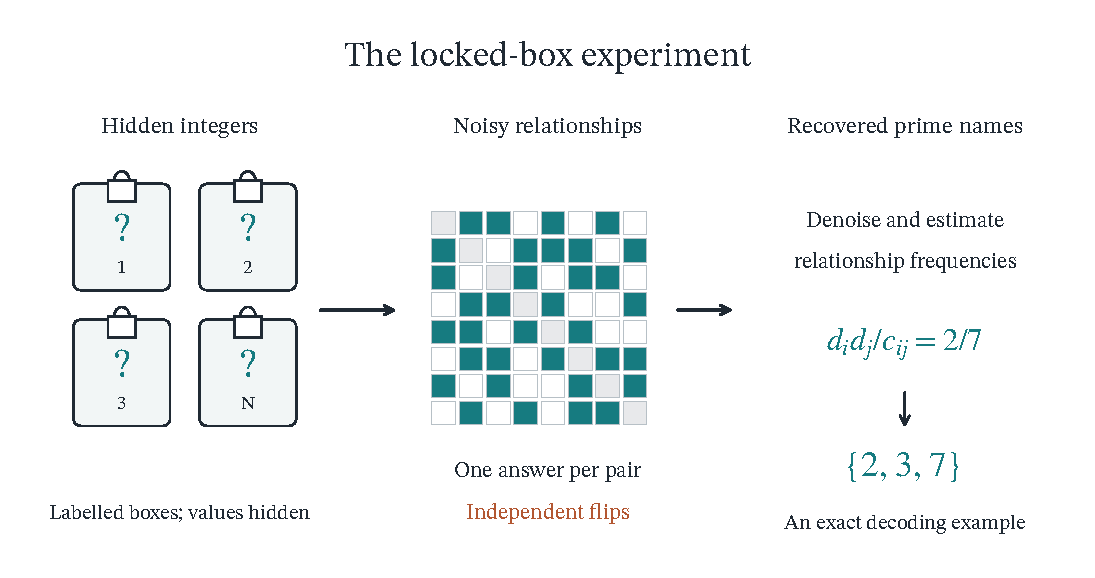
\includegraphics[width=\linewidth]{figures/04_locked_boxes.pdf}
 \caption{A schematic of the recovery experiment. The box identities
 remain aligned while their integer values are hidden. One independently
 corrupted coprimality bit is observed per unordered pair. The theorem
 recovers exact shared-prime sets on a fraction of pairs tending to one;
 this diagram makes no finite-sample accuracy claim. The exact ratio
 $2/7$ illustrates the decoder for the prime set $\{2,3,7\}$.}
 \label{rec:locked-boxes-figure}
\end{figure}

\begin{theorem}[The threshold for recovery on almost every pair]\label{rec:threshold}
There is a single procedure using $Y$ alone such that, whenever
$T_N\to\infty$, for every fixed pair $i\ne j$,
\[
 \Prob(\widehat R_{ij}=R_{ij})\longrightarrow1,
 \qquad
 \frac1{\binom N2}\sum_{i<j}\mathbf1_{\{\widehat R_{ij}\ne R_{ij}\}}
 \longrightarrow0\quad\hbox{in probability}.
\]
If $T_N$ does not tend to infinity, neither a vanishing error probability
for a fixed pair nor a vanishing fraction of pair errors is possible,
even if $\varepsilon_N$ is supplied. The same criterion holds in the
independent-prime model.
\end{theorem}

This is a sharp distinction. If the distance of the error rate from one
half is a constant times $N^{-1/2}$, some uncertainty about a fixed
pair persists. Multiply that distance by \emph{any} factor tending to
infinity, however slowly, and consistency becomes possible. The theorem
names the primes correctly on a proportion of pairs tending to one.
It gives no guarantee that every pair in a given table is correct.

\paragraph{How an approximate table gives exact names.}
There are three steps. First calibrate the noise using the average
coprimality frequency. Then use the repeated prime features to denoise
the whole matrix. Finally estimate the three frequencies for each pair
and search for the nearest admissible rational code. With a bound on
their denominators, distinct rationals have a positive separation;
the allowed bound grows slowly enough for the estimation error to fall
below that separation. A typical pair has a bounded common divisor
with high probability, so eventually its correct code enters the search.

The matrix step uses established singular-value thresholding
\cite{RecChatterjeeUSVT2015,RecXuSpectral2018}. The full construction and
all error estimates are in Appendix~\ref{rec:threshold-proof}. The
rational search there deliberately grows very slowly; the theorem is
an asymptotic result, with no practical sample-size guarantee.

There is also an elementary reason a weaker signal cannot suffice.
Imagine being told everything except whether one hidden odd number
$u$ has been replaced by $2u$. If its partner is even, that one choice
changes whether they share the prime $2$. Only the answers involving
the uncertain box can distinguish the choices. Their combined testing
strength is bounded when $T_N$ is bounded. Even this almost-completely
opened version of the game retains a positive error probability.

\subsection{Parity and every fixed finite prime profile}

The decoder identifies numerical prime names, so it can distinguish
even from odd. This is more concrete than recovering an unnamed group
of boxes that happen to resemble one another. A box containing a
multiple of $2$ shares $2$ with roughly half the other boxes. An odd
box shares $2$ with none. The decoded pair sets turn that difference
into a vote.

\begin{corollary}\label{rec:profiles}
Under $T_N\to\infty$, for each fixed prime cutoff $P$ the divisibility
bits $\mathbf1_{\{p\mid X_i\}}$, $p\le P$, can be recovered correctly
for a fraction of vertices tending to one. For each fixed vertex their
joint recovery probability tends to one. In particular the table
reveals the parity of almost every hidden integer.
\end{corollary}
\begin{proof}
For a fixed $p$, declare that $p\mid X_i$ when more than $N/(2p)$ of
the estimated $R_{ij}$ are divisible by $p$. The true number is zero
if $p\nmid X_i$, and otherwise it is the number of other sampled
multiples of $p$, which is $N/p+o_{\Prob}(N)$ simultaneously for all
such rows. On this event, a mistaken vertex bit requires at least
$N/(3p)$ pair errors in its row. Summing over rows proves a vanishing
vertex-error fraction; a finite union handles $p\le P$. Equivariance
gives the fixed-vertex assertion.
\end{proof}

For parity, the rule in the proof uses a threshold of $N/4$ shared-$2$
reports. The same idea recognizes multiples of $3$, of $5$, or of any
other fixed prime: the two limiting row frequencies are $0$ and $1/p$.
Putting finitely many of these tests together reveals patterns such as
``divisible by $3$ and $7$, but not by $2$ or $5$.'' These will shortly
recover the prime lanes of the original constant.

The fixed cutoff in the corollary matters. A prime occurring in only
one sampled integer has no shared-prime witness in the finite table.
And replacing a prime factor by a higher power changes none of its
coprimality relationships. The recovered arithmetic is the presence of
the specified primes.

Question~\ref{rec:prime-sample-question} asks for a practical version
of this recovery: how the required number of boxes depends on the
prime, the desired accuracy and the noise.

\subsection{Two ways to count what survives}

To compare recovery with information, use natural logarithms and let
$H(U)=-\sum_u\Prob(U=u)\log\Prob(U=u)$ for a discrete random object.
Mutual information is $I(U;V)=H(U)-H(U\mid V)$: the average reduction
in uncertainty about $U$ after observing $V$. With natural logarithms,
one fair binary choice has entropy $\log2$. All graph entropies below
include the vertex labels.

There are now two scores for the game. Pair accuracy gives one point
for each completely correct shared-prime set. The information fraction
\[
 \frac{I(G_N;Y_N)}{H(G_N)}
 =1-\frac{H(G_N\mid Y_N)}{H(G_N)}
\]
asks what proportion of the clean table's uncertainty the noisy table
has removed. A small value means that most of that original uncertainty
remains. The two scores need not move together.

\begin{theorem}[Information in noisy coprimality]\label{rec:information}
In the ordinary-integer model \eqref{rec:finite-model}, uniformly in
$\varepsilon_N\in[0,1]$,
\begin{equation}\label{rec:information-law}
 I(G_N;Y_N)=N\log(1+T_N)+O(N\log\log N).
\end{equation}
In particular
\begin{equation}\label{rec:graph-entropy}
 H(G_N)=N\log N+O(N\log\log N).
\end{equation}
\end{theorem}

The clean table has roughly $N^2/2$ entries but only about $N\log N$
units of uncertainty. Its entries are tied together by the hidden
integers. For comparison, the ordered list of those integers has entropy
exactly $2N\log N$. Since the clean table is determined by the list,
\eqref{rec:graph-entropy} says that it retains asymptotically half the
list's Shannon information.

At any fixed error rate different from one half, the noisy table retains
a fraction tending to one of the \emph{clean table's} information.
Thus even $49\%$ independent reversals leave nearly all of that fraction
in the limit. Letting the error rate approach one half gives a continuous
range of outcomes. For every fixed $0<\theta\le1$,
\[
 T_N=N^\theta
 \quad\Longrightarrow\quad
 \frac{I(G_N;Y_N)}{H(G_N)}\longrightarrow\theta.
\]
Meanwhile, prime-set recovery on almost every pair succeeds for every
one of these choices. Taking $\theta=1/100$ leaves asymptotically one
percent of the information, with the fraction of correctly decoded
pairs still tending to one. We can push the information fraction all
the way to zero by making $T_N$ grow more slowly.

The error in \eqref{rec:information-law} may exceed its displayed main
term for very small $T_N$. The proof also gives $I(G_N;Y_N)=O(N)$ when
$T_N$ stays bounded. We shall only use the uniform formula below to
obtain an upper bound, for which its error term suffices.

\begin{corollary}[Almost every answer, a vanishing information fraction]
\label{rec:paradox}
Take $\varepsilon_N=(1-\sqrt{\log N/N})/2$, so $T_N=\log N$.
Then a procedure recovers the exact shared-prime set for a fraction
of pairs tending to one, while
\begin{equation}\label{rec:paradox-limits}
 \frac{I(G_N;Y_N)}{H(G_N)}\longrightarrow0.
\end{equation}
\end{corollary}
\begin{proof}
The recovery conclusion follows from Theorem~\ref{rec:threshold}.
The numerator in \eqref{rec:paradox-limits} is $O(N\log\log N)$
by Theorem~\ref{rec:information}, whereas its denominator is
$N\log N+O(N\log\log N)$.
\end{proof}

This is the paradox named in the title. On almost every pair we recover
an exact list of numerical primes, although a fraction tending to one
of the clean table's original uncertainty remains unresolved.

\paragraph{Where can all that unresolved information hide?}
Fix a prime cutoff $P$. For any pair of our ordinary sampled integers,
\[
 \Prob(\text{the pair shares a prime larger than }P)
 \le\sum_{p>P}\frac1{p^2}\longrightarrow0.
\]
Thus the large primes can be ignored at a small cost in pair accuracy.
This remains true when ``correct'' requires the \emph{whole} shared-prime
set: a pair with no common prime above $P$ has no omitted part of its
answer. Letting the cutoff grow slowly is enough to cover almost all
pairs.

Uncertainty adds up differently. In the independent-prime model, the
entropy of one box's divisibility bits through $P$ grows like $\log P$;
the prime sum behind this is
$\sum_{p\le P}(\log p)/p\sim\log P$. There are many rare choices of
large prime, and the numerical identity of each choice carries
information. Their accumulated uncertainty can be substantial even
when their effects occupy few pairs. Appendix~\ref{rec:information-proof}
makes this comparison quantitative for ordinary integers, including
the dependence among their prime divisibilities.

Nor has the surviving information become small in absolute terms.
Parity recovery alone implies
\begin{equation}\label{rec:parity-information}
 I(G_N;Y_N)\ge N\log2-o(N)
 \qquad\text{whenever }T_N\to\infty.
\end{equation}
Indeed, the hidden parities are independent and asymptotically fair.
If their mean decoding error is $e_N\to0$, their conditional entropy
is at most $N h(e_N)=o(N)$, where
$h(t)=-t\log t-(1-t)\log(1-t)$. The data-processing inequality then
gives \eqref{rec:parity-information}. In the paradox regime we therefore
retain at least order $N$ information, while the clean table contains
order $N\log N$. The vanishing \emph{fraction} and successful pair
reconstruction fit together without losing this extensive amount of
recoverable arithmetic.

\section{Returning to the digits without their addresses}\label{rec:digits-return}

We have learned to identify prime divisibility without opening the
boxes. Put that knowledge back into the original digit construction.
This time a box contains a \emph{digit position}, and its visible mark
is the digit at that position. Shuffle the sampled positions out of
sight, corrupt the marks, and also corrupt the coprimality answers
between positions. The questions stored in the constant can still be
read.

The distinction between a box number and a digit position is essential.
Box $i$ remains identifiable throughout the experiment; its hidden
position $X_i$ does not. We observe which noisy mark belongs to which
row of the table. No ordering of the sampled digit positions is given.

Recall what a lane does. If its message bit is zero, every digit in
that lane is zero. If its bit is one, the Liouville parity rule makes
asymptotically half its digits equal to one. Once the graph has
identified the lane, this difference can be read by averaging its marks.
The individual numerical positions need never be reconstructed.

For a fixed mask $g$ with $g_1=1$, recall
\[
 x_g(1)=0,\qquad
 x_g(n)=\frac{1-\lambda(n)}2g_{\ell(n)}\quad(n\ge2),\qquad
 C_g=\sum_{n\ge1}x_g(n)2^{-n}.
\]
In addition to \eqref{rec:finite-model}, observe
\[
 Z_i=x_g(X_i)\mathbin{\oplus}B_i',\qquad
 B_i'\sim\operatorname{Bernoulli}(\eta_N),
 \qquad b_N=1-2\eta_N.
\]
All digit flips are mutually independent and independent of the integers
and edge flips. For the following finite theorem the digit-noise
probability $\eta_N$ is supplied; the edge-noise probability remains
unknown.

The two channels have different jobs. The edge signal $a_N$ lets us
sort boxes into prime lanes. The digit signal $b_N$ lets us distinguish
an enabled lane from a disabled one after that sorting. Neither channel
has to stay a fixed distance from a fair coin.

\begin{theorem}[Recovering the arithmetic message]\label{rec:message}
If $Na_N^2\to\infty$ and $Nb_N^2\to\infty$, a single procedure
recovers each fixed bit $g_j$ with probability tending to one, while
recovering the exact common-prime sets on a fraction of pairs tending
to one. It gives an estimator $\widehat C_N\to C_g$ in probability.
The two signal conditions are jointly necessary for one procedure to
have these joint consistency properties for every fixed mask with
$g_1=1$.
\end{theorem}

\paragraph{Reading a message bit.}
To read $g_j$, select the boxes whose contents are divisible by $p_j$
and by no smaller prime. Corollary~\ref{rec:profiles} identifies this
set with a vanishing fraction of mistakes. It contains asymptotically
$\delta_jN$ boxes, where $\delta_j>0$ is the familiar lane density.
After correcting the known digit noise, average their signs
$(1-2Z_i)/b_N$. The average tends to $1-g_j$: zero for an enabled lane,
one for a disabled lane. Rounding recovers the message bit.

For example, the lane of $5$ is recognized by divisibility by $5$ and
nondivisibility by $2$ and $3$. Before noise, an enabled lane has
one-frequency $1/2$, whereas a disabled lane has one-frequency $0$.
After noise these become $1/2$ and $\eta_N$. The signal condition says
that the separation remains detectable by pooling the growing lane.
For the actual Goldbach message, the bit carried by $5$ is already
known from $8=3+5$; the same reading procedure applies to every fixed
lane, however far along the prime list it lies.

Recovering each fixed finite collection of message bits recovers each
fixed initial block of the constant. The total contribution of binary
digits beyond position $M$ is at most $2^{-M}$, so the estimates converge
to the entire real number. Appendix~\ref{rec:message-proof} gives the
full construction and proves necessity of both signals for the joint
task in the theorem.

\subsection{Knowing the Liouville signs does not solve the game}

The digit construction uses the parity of the number of prime factors.
It is natural to ask how much that extra arithmetic helps to identify
shared primes. Suppose an oracle now reveals every exact Liouville
sign. The recovery threshold is unchanged.

\begin{corollary}\label{rec:liouville-oracle}
Supplying all exact Liouville signs $\lambda(X_i)$ does not lower
the common-prime recovery threshold. More generally, supplying all
$\Omega(X_i)\bmod r$ for any fixed integer $r\ge2$ leaves the
threshold $Na_N^2\to\infty$ unchanged.
\end{corollary}
\begin{proof}
For the first assertion use $u$ and $4u$ as above. For the second use
$u$ and $2^ru$, with $u$ odd and $u\le N^2/2^r$. The paired event
has limiting probability $2^{-r}>0$, the residue of $\Omega$ is the
same, and presence of the prime 2 differs. The identical testing
argument applies. Sufficiency already holds without the extra data.
\end{proof}

The small witness in this proof is worth keeping in view. Multiplying
an odd integer by $4$ preserves its Liouville sign while adding the
prime $2$ to its prime support. Multiplying by $2^r$ does the same while
preserving $\Omega$ modulo $r$. These two kinds of parity---how many
prime factors there are, and whether $2$ occurs at all---encode different
information.

The word ``joint'' in Theorem~\ref{rec:message} matters. Its necessary
edge threshold concerns a task that also reconstructs common-prime
sets. At the level of limiting digit frequencies, the balance law
already distinguishes the all-one message from a message with a
disabled lane. Naming the individual disabled lanes demands more
information.

Recovering just the message could require less edge information.
Question~\ref{rec:message-only-question} isolates this task while
keeping the digit-noise rate supplied to the procedure.

\subsection{Goldbach becomes a question of independence}

One more question brings us directly back to Goldbach. Imagine looking
at a single visible digit mark. Can knowing the entire graph change
the probability that this mark is one? In the limiting experiment,
Goldbach says precisely that it cannot.

The reason is the lane mechanism. When every lane is enabled, every
mark is a fair bit independently of the prime profile. A disabled
lane gives its marks a different distribution. The graph can identify
that lane, so it can predict something about the marks. A single
Goldbach exception would create statistical dependence between the
digits and the relationships among their hidden addresses.

Here is the exact experiment, with fixed noise rates.
Let the profiles $S_i$ be as in Section~\ref{rec:relationships}, let
$J_i$ be their least-prime index, and let $V_i$ be independent fair
bits independent of every profile. Give vertex $i$ the clean label
$V_i g_{J_i}$ and flip it with a fixed probability $\eta\ne1/2$.
Independently flip graph edges with a fixed $\varepsilon\ne1/2$.
Both rates may be unknown.

This is the limit of every fixed finite ordinary-integer marked
experiment. For a fixed prime-divisibility pattern, expand its indicator
by inclusion--exclusion. Each Liouville-weighted term is
$\lambda(d)L(X/d)=o(X)$ for a fixed integer $d$. Thus the Liouville
sign becomes a fair bit independent of the finite profile. The
least-prime tail has probability at most
$\prod_{p\le R}(1-1/p)\to0$, and the shared-prime tail is controlled
as before. Taking the range limit and then the prime cutoff proves
the assertion. This does not identify consecutive-digit frequencies.

\begin{proposition}\label{rec:infinite-message}
In this countable limiting model, the noisy marked graph determines
the whole mask almost surely. For the Goldbach mask, one observed
label is independent of the entire observed graph if and only if
Goldbach holds.
\end{proposition}
\begin{proof}
Equations \eqref{rec:infinite-noise}--\eqref{rec:epsilon} and
Theorem~\ref{rec:frequency} recover every profile. Each lane has
positive probability $\delta_j$, so its observed label frequency is
almost surely $1/2$ when $g_j=1$ and $\eta$ when $g_j=0$.
Since $\eta\ne1/2$, these exact limiting frequencies recover all bits,
even if $\eta$ is unknown.

Let $\mathscr G$ be the sigma field of the observed infinite graph,
put $S=\sum_{j:g_j=0}\delta_j$ and $b=1-2\eta$. The recovered lane
of a fixed vertex is $\mathscr G$-measurable, and its observed label
$Z_i$ satisfies
\[
 \Prob(Z_i=1\mid\mathscr G)=
 \begin{cases}
  1/2,&g_{J_i}=1,\\
  \eta,&g_{J_i}=0.
 \end{cases}
\]
Its conditional entropy is therefore $\log2$ in an enabled lane and
$h(\eta)$ in a blocked lane. Consequently,
\begin{equation}\label{rec:label-information}
 I(Z_i;\mathscr G)
 =h\left(\frac{1-bS}{2}\right)
  -(1-S)\log2-S h(\eta).
\end{equation}
The enabled 2-lane makes $1-S>0$. Strict concavity of $h$ shows that
\eqref{rec:label-information} is zero precisely when $S=0$, because
$\eta\ne1/2$. For the Goldbach mask, $S=0$ is equivalent to Goldbach.
\end{proof}

When Goldbach holds, the entire label sequence is independent fair
bits, independent of the graph, and the label-noise rate is
unidentifiable in this limiting model. Fixed-pattern convergence does
not transfer that exact unidentifiability statement to growing
$N$-vertex experiments with range $N^2$.

The message was repeated throughout its least-prime lanes. Coprimality
lets us find those repetitions without their numerical addresses, and
averaging lets us read them through noise. The same lane structure
therefore appears in three concrete forms: a balance law for the
constant, a recoverable message on hidden integers, and an independence
criterion for Goldbach in the limiting experiment.

\begin{remark}[Relation to other reconstruction problems]
Feature reconstruction in random intersection graphs and statistical
information/recovery comparisons are established subjects. In
particular, Göbel, Ruff and Schiller~\cite{RecGobelRuffSchiller2026}
study efficient, robust recovery in a homogeneous growing-feature
model. Our features have probabilities $1/p$, are numerically
identified, and arise from ordinary sampled integers in the main
theorems. The precise target here is recovery of shared primes on a
fraction of pairs tending to one, under independent common-rate flips.
\end{remark}

\section{Choosing integers that do not share primes}\label{fin:selection}
Put the integers $2,3,\ldots,X$ on cards.  We may keep as many cards
as we like, provided no two kept cards share a prime factor.
Thus $8$ and $9$ can sit together; $6$ and $10$ cannot.
The prime $2$ is a resource that the second pair tries to spend twice.

Now choose an admissible collection uniformly at random.
How many cards does it contain?  The cards interact in a complicated
way, but the answer is almost the size of a pile of independent fair
coin flips.  Better still, an independent binomial part can be extracted
\emph{exactly}, before taking any limit.

\subsection{A small example with a coin inside}
For the five cards $2,3,4,5,6$, the admissible collections have
generating polynomial
\[
 1+5z+6z^2+2z^3=(1+z)(1+4z+2z^2).
\]
The coefficient of $z^j$ counts the collections of size $j$.
There are fourteen collections in all, including the empty one.
The factor $1+z$ has an immediate explanation: the card $5$ shares
no prime with any other card, so it can be added or removed freely.
A uniformly chosen collection therefore contains this card according
to an independent fair coin.

For a larger interval the free coins need not have fixed names.
Choosing a composite card may use up prime cards that would otherwise
be available.  Nevertheless, a large binomial component survives in
the \emph{distribution of the number of cards kept}.

To include later deletion experiments, let $B$ be any set of allowed
primes.  Write $\mathcal N_B(X)$ for the integers in $[2,X]$ whose
prime divisors all belong to $B$, and define
\[
 P_{B,X}(z)=\sum_{\substack{S\subseteq\mathcal N_B(X)\\
                       S\ {\rm pairwise\ coprime}}}z^{|S|}.
\]
Here $N_B=\#(B\cap[2,X])$ counts available prime cards,
$r_B=\#(B\cap[2,\sqrt X])$ counts the small ones, and
\[
 m_B=\max(0,N_B-2r_B),\qquad d_B=N_B-m_B.
\]
\begin{theorem}[The binomial component]\label{fin:binomial}
There is a polynomial $Q_{B,X}$ with nonnegative integer coefficients,
of degree $d_B$, such that
\[
 \boxed{P_{B,X}(z)=(1+z)^{m_B}Q_{B,X}(z).}
\]
Give each admissible subset probability proportional to
$\lambda^{|S|}$, where $\lambda>0$, and put
$\theta=\lambda/(1+\lambda)$.  Its size has the exact distribution
\begin{equation}
 |S|\ \overset d=\ Z+R,\qquad
 Z\sim\operatorname{Binomial}(m_B,\theta),\quad
 0\le R\le d_B,\quad Z\ \text{independent of }R.
 \label{fin:coinrepresentation}
\end{equation}
\end{theorem}
\begin{proof}
First choose the composite members $T$ of an admissible subset.
Let $u(T)$ count the distinct primes occurring in them.  Every remaining
prime through $X$ can then be included or excluded freely, giving
\begin{equation}
 P_{B,X}(z)=\sum_T z^{|T|}(1+z)^{N_B-u(T)}.                 \label{fin:splitpoly}
\end{equation}
Every composite through $X$ uses a prime at most $\sqrt X$ and at most
one distinct prime greater than $\sqrt X$.  Since the members of $T$
have disjoint prime supports,
\[
 |T|\le r_B,\qquad |T|\le u(T)\le r_B+|T|\le2r_B.
\]
Factor $(1+z)^{m_B}$ out of each summand.  The remaining terms have
nonnegative coefficients and degree at most $N_B-m_B$.
Choosing all available primes shows that $P_{B,X}$ has degree $N_B$,
so the quotient has degree exactly $d_B$.
Finally,
\[
 \E t^{|S|}
 =\left(\frac{1+\lambda t}{1+\lambda}\right)^{m_B}
   \frac{Q_{B,X}(\lambda t)}{Q_{B,X}(\lambda)}
\]
is the product of two probability generating functions, which proves
the claimed independent representation.
\end{proof}

The proof explains the abundance of coins.  Every composite spends a
small prime, and different selected composites must spend different
small primes.  There are too few small primes to entangle most of the
available choices.

Taking $\lambda=1$ makes all admissible collections equally likely.
The following stronger approximation says that \emph{every} event
concerning the selected size has almost the same probability as in the
binomial model.  The distance $d_{\mathrm{TV}}$ is the largest
difference between such event probabilities.
\begin{corollary}\label{fin:binomialtv}
If $N_B(X)\sim\pi(X)$, then, for fixed $\theta\in(0,1)$,
\[
 d_{\mathrm{TV}}\bigl(\mathcal L(|S|),
                 \operatorname{Binomial}(N_B(X),\theta)\bigr)
 =O_\theta((\log X)^{-1/2}).
\]
The proportion of roots of $P_{B,X}$ that equal $-1$, counted with
multiplicity, tends to one.  The integer $P_{B,X}(1)$ is divisible by
$2^{m_B}$.
\end{corollary}
The short smoothing estimate is in Appendix~\ref{finapp:binomial}.

For the full prime set, the trial count is $\pi(X)$.
A large, highly constrained family of subsets therefore has the size
profile of $\pi(X)$ fair coins.  The factorization leaves two further
fingerprints: almost every polynomial root is exactly $-1$, and
the total number of admissible collections has a large power of two
as a divisor.  These are three readings of the same free choices.

\subsection{An order that almost ceases to matter}
A greedy choice can depend strongly on its order.
From the cards $6,10,9$, taking $6$ first leaves a collection of size
one; taking $10$ and then $9$ gives size two.
The next experiment has a surprising large-sample answer:
nearly all of a maximal collection is forced before we choose an order.

Sample $N$ labelled integers independently and uniformly from
$[1,\lfloor N^\beta\rfloor]$, with fixed $\beta>1$.
Repeated values keep separate labels.  Let $\alpha_N$ be the largest
pairwise-coprime selection size.  Let $\mathcal U_N$ be the labels
coprime to every other sampled label.  Such a label can be added to
any admissible collection, so every inclusion-maximal collection
must contain it.

The answer involves Buchstab's function $\omega$, which measures the
frequency of integers with no small prime factor.
For $1<\beta\le2$, $\omega(\beta)=1/\beta$; its full definition is
given in Appendix~\ref{finapp:greedy}.
\begin{theorem}[A compulsory part of every answer]\label{fin:greedy}
In the preceding random-input model,
\[
 |\mathcal U_N|\sim\alpha_N\sim
 \omega(\beta)\frac{N}{\log N}
 \quad\text{in probability}.
\]
Uniformly over every pair $S,T$ of inclusion-maximal coprime selections,
\[
 |S\mathbin{\triangle}T|=o_{\Prob}(N/\log N).
\]
Consequently every greedy ordering is asymptotically optimal, even when
the order is chosen after the entire sample is seen.
\end{theorem}

For example, sampling from $[1,N^2]$ gives a largest collection of
size asymptotic to $N/(2\log N)$.
Even an adversary who sees the entire sample before choosing the
greedy order cannot lose a positive fraction of that answer.

The reason is concrete.  Numbers made only from primes above $N$
rarely share any of those primes with another sampled number.
They supply the compulsory set $\mathcal U_N$.
Meanwhile every selected number using a small prime must spend a
different small prime.  Counting those resources bounds what can be
added beyond $\mathcal U_N$.  The two bounds meet; the estimates are
in Appendix~\ref{finapp:greedy}.

\subsection{A crowd can avoid collisions and leave more holes}
Keep the prime-feature model, but reverse the experiment.
Choose $n$ independent integers from $[1,X]$ and condition them to be
pairwise coprime.  We first let $X\to\infty$ with $n$ fixed, and only
then let the crowd grow.

A prime can now belong to at most one crowd member.  One might expect
this economical use of primes to produce especially thorough coverage.
In fact the first missing prime arrives on a much smaller scale.

The effect is visible before any asymptotics.  An ordinary crowd is all
odd with probability $2^{-n}$.  A pairwise-coprime crowd is all odd
with probability $1/(n+1)$.  With three members the probabilities are
$1/8$ and $1/4$, respectively.

At each prime $p$, the limiting probabilities are
\[
 \Prob(p\text{ absent})=\frac{p-1}{n+p-1},\qquad
 \Prob(p\text{ belongs to a specified member})=\frac1{n+p-1}.
\]
Different primes are independent in this limit.
For finitely many primes this follows from the Chinese remainder
theorem; the chance of a shared prime above a cutoff $z$ is at most
$\binom n2\sum_{p>z}p^{-2}$, which justifies removing the cutoff.
\begin{proposition}[The first missing prime]\label{fin:coverage}
Let $L_n$ be the smallest prime absent from the crowd.  In the coprime
experiment,
\[
 \frac{L_n}{\sqrt{n\log n}}\ \Longrightarrow R,
 \qquad \Prob(R>t)=e^{-t^2}\quad(t\ge0).
\]
For an ordinary unconditioned crowd, $L_n\sim n/\log n$ in probability.
More precisely,
\[
 \frac n{L_n}-\log n+3\log\log n\Longrightarrow G,
 \qquad \Prob(G\le t)=e^{-e^{-t}}.
\]
\end{proposition}

Here $L_n$ records the first hole in the crowd's prime coverage.
The coprime crowd finds its first hole around $\sqrt{n\log n}$;
the ordinary crowd reaches the much larger scale $n/\log n$.
The limit laws describe the fluctuations around these scales
(Appendix~\ref{finapp:crowds}).
Avoiding repeated ownership does not make ownership more complete.

\subsection{One probability, two experiments}
Inspect the crowd already assembled.  Does its product contain any
repeated prime power?  Now perform a different experiment: invite one
fresh integer, with no conditioning on the newcomer.  Is it coprime
to everyone present?

These events have exactly the same probability.
The equality joins an internal property of the old crowd to the
admission chance of a new member.
\begin{proposition}[Old powers and a new member]\label{fin:powers}
In the same iterated limit,
\[
 \Prob(\text{crowd product squarefree})
 =\Prob(\text{a fresh integer is coprime to the crowd})
 =\frac{K(n+1)}{K(n)}.
\]
For fixed $r\ge3$, as $n\to\infty$,
\[
 \Prob(\text{crowd product is }r\text{-free})\longrightarrow
 \frac1{\zeta(r-1)}.
\]
In particular the cube-free probability tends to $6/\pi^2$, whereas
the squarefree probability tends to zero.
\end{proposition}
\begin{proof}
Given that $p$ is present, its unique owner's valuation has distribution
$\Prob(v_p=j)=(1-1/p)p^{-(j-1)}$ for $j\ge1$.  Thus the probability
that $p^r$ divides the product is
$n/[p^{r-1}(n+p-1)]$.  For $r=2$, multiplying the complementary
probabilities gives $K(n+1)/K(n)$, as does the conditional probability
of admitting a new member.  For $r\ge3$, dominated convergence of the
Euler product gives the zeta value.  The squarefree probability tends
to zero since, for any fixed cutoff, its limiting product is at most
$\prod_{p\le z}(1-1/p)$, which tends to zero as $z\to\infty$.
\end{proof}

There is a second surprise in the last limit.  As the crowd grows,
being squarefree becomes unlikely, but being cube-free retains the
positive probability $6/\pi^2$.  A crowd can accumulate repeated
primes while still usually avoiding high repetitions.

We can also keep a record of precisely what was repeated.
For crowd product $M$, put
\[
 D_n=\frac{M}{\rad(M)},
\]
where $\rad(M)$ keeps one copy of each prime.
For example, the pairwise-coprime crowd $72,25,7$ has
$M=2^3 3^2 5^2 7$ and $D_n=2^2\cdot3\cdot5=60$.
The exact limiting law is
\begin{equation}\label{fin:remainderlaw}
 \Prob(D_n=d)=\frac{K(n+1)}{K(n)}\,\frac1d
                    \prod_{p\mid d}\frac n{n+p}.
\end{equation}
Thus the excess powers have a probability law of their own, although
the integers in the original experiment grow without bound.

On a logarithmic scale this remainder meets the classical Dickman law.
\begin{corollary}[A small remainder]\label{fin:dickman}
Let $Y$ have Laplace transform
\[
 \E e^{-sY}=\exp\left(\int_0^1\frac{e^{-st}-1}{t}\,dt\right).
\]
Then $\log D_n/\log n\Longrightarrow Y$, and
$\Prob(D_n\le n)\to e^{-\gamma}$.
\end{corollary}
The local valuation calculation and the limit proof are in
Appendix~\ref{finapp:crowds}.

In particular, the chance that all repeated material fits below the
crowd size tends to $e^{-\gamma}\approx0.56146$:
\[
 \Prob(D_n\le n)\longrightarrow0.56146\ldots.
\]
The crowd size, rather than the much larger sampled integers, sets
the natural scale for its repeated prime material.

\section{What an average can hide}\label{fin:matrices}
There are two ways to average a spectrum.
We can find the eigenvalues in every experiment and average their
histograms.  Or we can average the characteristic polynomials first
and then find the roots.  These operations can tell different stories.

A two-dimensional example makes the distinction visible.
With equal probability take
\[
 A_1=\begin{pmatrix}0&0\\0&2\end{pmatrix},
 \qquad
 A_2=\begin{pmatrix}2&0\\0&4\end{pmatrix}.
\]
The averaged eigenvalue histogram puts mass $1/4,1/2,1/4$ at
$0,2,4$.  But the average characteristic polynomial is
\[
 \frac12z(z-2)+\frac12(z-2)(z-4)=(z-2)^2.
\]
Its two roots agree.  Averaging the polynomial has hidden the spread.

Our coprimality probabilities produce an exact, large-dimensional
version of this distinction, tied to the prime--composite
factorization from the earlier chapters.

\subsection{A polynomial made from chances of coprimality}
Recall that $K(k)$ is the limiting probability that $k$ random
integers are pairwise coprime.  Form
\[
 J_N(z)=\sum_{k=0}^N\binom Nk K(k)z^k.
\]
If we sample $N$ labelled integers and count their admissible
subcollections by size, $J_N$ is the limiting \emph{expected} counting
polynomial.  The factor $\binom Nk$ chooses the labels, and $K(k)$
is the chance that those labels are compatible.

This is a different object from $P_{B,X}$, which counts choices in a
fixed interval of integers.  All roots of $J_N$ are negative and real;
write them as $-R_{N,1},\ldots,-R_{N,N}$.
The prime-by-prime real-root argument is given in
Appendix~\ref{finapp:matrix}.

Let $\Comp$ be the composite product from the exponential factorization,
so $\E \Comp^s=\Gamma(s+1)K(s)$ for $s>-1$.
To build the matrix experiment, favor larger values of $\Comp$ by
multiplying the probability weight of a value $c$ by $c^N$ and
renormalizing.  This gives the scalar $\CompN $ below.
\begin{theorem}[Roots of the average versus typical eigenvalues]
\label{fin:wishart}
Let $Z_N$ have independent standard complex Gaussian entries
($\E|Z_{ij}|^2=1$), and independently let $\CompN $ have distribution
$c^N\,d\Prob_{\Comp}(c)/(N!K(N))$.  Put $V_N=Z_NZ_N^*/\CompN $.
Then
\[
 \E\det(zI-V_N)=(-1)^N\frac{J_N(-z)}{K(N)}
              =\prod_{j=1}^N(z-R_{N,j}).
\]
With $a_N=e^\gamma\log N$,
\[
 \frac1N\sum_j\delta_{R_{N,j}/a_N}\Longrightarrow\delta_1,\qquad
 \frac1N\sum_j\delta_{\lambda_j(V_N)/a_N}
       \Longrightarrow\operatorname{MP}_1
       \quad\text{in probability},
\]
where $\operatorname{MP}_1$ has density
$(2\pi)^{-1}\sqrt{(4-x)/x}$ on $(0,4)$.
\end{theorem}

Read the first limit as follows: after dividing by $e^\gamma\log N$,
almost all roots of the averaged polynomial gather near $1$.
The second limit says that a typical matrix has a whole spread of
eigenvalues across $(0,4)$ on that very same scale.

The distribution of $\CompN $ uses the composite factor already paired with
our prime product, and the identity follows from its moments.
Expanding Gaussian minors gives factorials; the identity
$\E \Comp^k=k!K(k)$ supplies precisely the arithmetic coefficients.
Appendix~\ref{finapp:matrix} gives the calculation and both limits.

\subsection{The hidden spread is a triangular spectrum}\label{tri:section}
The roots of $J_N$ have just collapsed to one point after division by
$e^\gamma\log N$.  That does not mean they have become equal.
It means we have chosen a scale on which their interesting differences
are hard to see.

A finer view reveals a familiar shape from an apparently distant
experiment.  Fill the region above a matrix diagonal with independent
complex Gaussian entries of variance $1/N$, and put zeros elsewhere:
\[
 \mathsf T_N=
 \begin{pmatrix}
 0& *& *&\cdots& *\\
 0& 0& *&\cdots& *\\
 \vdots&\vdots&\ddots&\ddots&\vdots\\
 0&0&\cdots&0&*\\
 0&0&\cdots&0&0
 \end{pmatrix}.
\]
All eigenvalues of this triangular matrix are zero.
Its singular values still measure how strongly it stretches vectors.
Their squares are the eigenvalues of $\mathsf T_N^*\mathsf T_N$;
these have a nontrivial limiting histogram.

That histogram is the Dykema--Haagerup law
$\operatorname{DH}_1$, supported on $[0,e]$
\cite{triDykemaHaagerup,triCheliotis}.
Its moments are
\[
 \int y^k\,d\operatorname{DH}_1(y)=\frac{k^k}{(k+1)!}
 \qquad(k=1,2,\ldots),
\]
so its mean is $1/2$.
No triangular matrices occur in the definition of $J_N$.
Nevertheless its roots reproduce this same law.

\begin{theorem}[The triangular spectrum]\label{tri:main}
Write $-R_{N,1},\ldots,-R_{N,N}$ for the roots of $J_N$,
with multiplicity. Center their positive magnitudes by setting
\[
 t_{N,j}=e^{-\gamma}R_{N,j}-\log N-\log\log N.
\]
Then
\begin{equation}\label{tri:exp}
 \boxed{\frac1N\sum_{j=1}^N
 \delta_{\exp(t_{N,j})}
 \Longrightarrow\operatorname{DH}_1.}
\end{equation}
Equivalently, if $T$ is the logarithm of a random variable with law
$\operatorname{DH}_1$, then
\begin{equation}\label{tri:centered}
 \frac1N\sum_{j=1}^N
 \delta_{t_{N,j}}
 \Longrightarrow\mathcal L(T).
\end{equation}
The law of $T$ has support $(-\infty,1]$; its explicit density is
given in \eqref{tri:density}.
\end{theorem}

Here is a practical reading of the theorem.
List the positive magnitudes of the arithmetic roots.
Multiply them by $e^{-\gamma}$, subtract
$\log N+\log\log N$, and make a histogram.
The result approaches a fixed asymmetric shape.
Exponentiate the centered entries, and the shape becomes the
squared-singular-value histogram of triangular Gaussian noise.

The common centering matters.
Dividing by $\log N$ erases fluctuations on a constant scale;
subtracting both $\log N$ and $\log\log N$ exposes them.
The extra $\log\log N$ is part of the arithmetic calculation.

\paragraph{Where the bridge comes from.}
The proof has three steps, all supplied in Appendix~\ref{triapp:all}.
First form the entire function
\[
 \mathcal E(z)=\sum_{k\ge0}K(k)\frac{z^k}{k!}.
\]
Its zeros are negative.  If their magnitudes are $\rho_j$, the prime
number theorem leads to the counting law
\[
 \#\{j:\rho_j\le r\}\sim e^{-\gamma}\frac r{\log^2r}.
\]
Second, Campbell and Jalowy's transfer theorem
\cite[Corollary 2.3]{finCampbellJalowy} turns this growth of the
entire function's zeros into a limiting law for the polynomial roots.
Finally, the precise arithmetic centering identifies that law as the
logarithm of $\operatorname{DH}_1$, using the identification of
Arizmendi and Hasebe \cite[Proposition 4.4]{triArizmendiHasebe}.

The connection therefore has a definite route:
coprimality probabilities determine an entire function;
its supply of zeros determines a free-stable law;
exponentiating that law gives the triangular spectrum.
The external transfer theorem supplies the bridge.
The prime estimates determine which law and which scale cross it.

The histogram alone does not locate the largest arithmetic root.
Question~\ref{tri:edgequestion} asks whether it also reaches the edge
of the triangular spectrum.


\section{A bell curve inside a rare factorization}\label{fin:entropy}
So far a prime factor has been a resource: present or absent, available
or spent.  Its size gives a different way to read the same integer.

Compare $72=8\cdot9$ with $2^{100}\cdot3$.
Both have two distinct prime factors.  In the first, the two prime-power
parts contribute almost equally to the logarithm.
In the second, the factor $3$ contributes very little.
Counting both examples as \emph{two factors} misses that difference.

For $n=\prod p^{a_p}$, give its prime-power parts logarithmic shares
\[
 w_p(n)=\frac{a_p\log p}{\log n}.
\]
These shares add to one.  Their entropy and effective factor count are
\[
 H(n)=-\sum_{p\mid n}w_p(n)\log w_p(n),\qquad D(n)=e^{H(n)}.
\]
At $n=1$ we set $H(1)=0$ and $D(1)=1$.
If $k$ shares are equal, then $D(n)=k$.
Unequal shares reduce the effective count:
\[
 D(72)\approx1.99924,\qquad
 D(2^{100}\cdot3)\approx1.08371.
\]
Every prime power has effective count one, however large its exponent.

\subsection{Infinitely many small factors, about three effective ones}
Choose an integer uniformly from $[1,N]$ and let $N$ grow.
The expected number of distinct prime factors tends to infinity:
divisibility counting and Mertens' theorem give
\[
 \E\,\#\{p:p\mid U_N\}
 =\sum_{p\le N}\frac{\lfloor N/p\rfloor}{N}
 \sim\log\log N.
\]
Yet its mean effective factor count approaches a finite number,
\[
 \boxed{\E D(U_N)\longrightarrow
       \mathfrak P=2.9621\ldots.}
\]
An integer gains more and more prime factors without gaining an
unbounded number of equally important logarithmic contributions.

The limiting shares have the classical
Poisson--Dirichlet law $\operatorname{PD}(0,1)$.
One way to make them is to break off a uniform fraction of a stick,
then a uniform fraction of the remainder, and continue.
Sort the resulting pieces into decreasing order.
The same law describes the limiting normalized cycle lengths of a
uniform random permutation
\cite[remarks after Theorem 1, part (d)]{finHaddadKoukoulopoulos}.
This is a classical prime-factor and
permutation connection, used here to ask about the shapes of unusually
balanced factorizations.

Write $P=(P_i)$ for this random partition and put
\[
 H=-\sum_iP_i\log P_i,\qquad D=e^H.
\]
Its mean entropy is exactly $1$, so $e^{\E H}=e$.
Averaging the effective count instead gives $\E e^H=\mathfrak P$.
The two numbers differ because exponentiating and averaging do not
commute.

These limiting statements also respect our choice to group repeated
copies of a prime into one prime-power part.
Lemma~\ref{fin:entropycoupling} makes that step quantitative.
Appendix~\ref{finapp:entropy-coupling} proves it and gives a positive
recursion for $\mathfrak P$ with an explicit truncation error.
Thus the displayed constant is computationally accessible as well as
probabilistically defined.

\subsection{What does an unusually large effective count cost?}
The event $D>x$ asks for the equivalent of more than $x$ substantial,
well-balanced factors.  It is much rarer than merely having more than
$x$ distinct prime divisors.
Sawin \cite[Lemma 9.5]{finSawin} bounded this same limiting entropy tail
by a constant times $x^{9/2}e^{2x}x^{-x}$.
Our expansion identifies its next logarithmic terms.
\begin{theorem}[A sharp entropy tail]\label{fin:entropytail}
As $x\to\infty$,
\[
 \boxed{-\log\Prob(D>x)
 =x\left(\log x+\frac12\log\log x
              -1-\frac12\log(2\pi)+o(1)\right).}
\]
\end{theorem}

Equivalently,
\[
 \Prob(D>x)=
 \left(\frac{e\sqrt{2\pi}}{x\sqrt{\log x}}\right)^x e^{o(x)}.
\]
The main rarity cost is $x^{-x}$.
Balancing the factors adds the further factor
$(\log x)^{-x/2}$.  The appearance of $\sqrt{2\pi}$ hints at the
geometry behind this balancing penalty.

Here is the idea of the proof.  To have effective count just above
$x$, a partition can use about $x$ pieces of size close to $1/x$.
Near equal shares, the entropy loss is approximately a quadratic
sum of their deviations.  Counting a thin region around this balanced
configuration gives a Gaussian volume.  A matching exponential bound
shows that configurations elsewhere cannot improve the leading cost.
The full upper and lower estimates are in
Appendix~\ref{finapp:entropy-tail}.

\subsection{The rare factors arrange themselves into a Gaussian}
The tail estimate says how unlikely balance is.
The next theorem says what balance usually looks like once we have
insisted on it.

Take a factor share $P_i$, compare it with $1/x$, and magnify the
relative difference by $\sqrt{\log x}$:
\[
 y_i=\sqrt{\log x}\,(xP_i-1).
\]
Give the point $y_i$ weight $P_i$.
The resulting histogram has total mass one.
Conditioned on $D>x$, this histogram approaches the familiar bell curve.
\begin{theorem}[A Gaussian profile]\label{fin:entropyprofile}
Given $D>x$, the random probability measure
\[
 \nu_x=\sum_i P_i\,\delta_{\sqrt{\log x}(xP_i-1)}
\]
converges weakly in probability to the standard Gaussian law.
For each bounded interval $(a,b)$,
\[
 \frac1x\#\{i:a<\sqrt{\log x}(xP_i-1)<b\}
 \longrightarrow \Phi_{\mathrm G}(b)-\Phi_{\mathrm G}(a)
\]
in the same conditional probability, where $\Phi_{\mathrm G}$ is the
standard Gaussian distribution function.
\end{theorem}

For example, asymptotically about $68.3\%$ of the logarithmic mass
lies in shares between
\[
 \frac{1-1/\sqrt{\log x}}x
 \quad\hbox{and}\quad
 \frac{1+1/\sqrt{\log x}}x.
\]
The number of shares in this window, divided by $x$, approaches the
same Gaussian proportion.
The bell curve describes fluctuations \emph{inside one rare
factorization}, rather than fluctuations between independently
sampled integers.

This conclusion is stronger than the symmetric construction used for
the tail lower bound.  That construction showed one economical way
to be unusually balanced.  The conditional theorem says that the
Gaussian shape is what the whole rare event typically selects.
Its proof, including exponential control of deviations, is in
Appendix~\ref{finapp:entropy-profile}.

\subsection{How far can we return to ordinary integers?}
For an actual integer $n$, a share near $1/x$ means that its corresponding
prime-power part is near $n^{1/x}$ on a logarithmic scale.
The limiting picture therefore suggests many comparably important
prime-power parts, with the preceding Gaussian pattern in their
logarithmic sizes.

A coupling with ordinary integers lets the threshold $x$ grow with
the sampling range.  The following is the range justified here.
\begin{corollary}\label{fin:integerentropy}
Fix $\epsilon>0$.  If $x=x(N)\to\infty$ and
\[
 x\le(1-\epsilon)\frac{\log\log N}{\log\log\log N},
\]
then the tail formula of Theorem~\ref{fin:entropytail} holds with
$D(U_N)$ in place of $D$.  Given $D(U_N)>x$, the measure
\[
 \sum_{p\mid U_N}w_p(U_N)
       \delta_{\sqrt{\log x}(xw_p(U_N)-1)}
\]
converges weakly in probability to the standard Gaussian law.
\end{corollary}
The transfer proof is in Appendix~\ref{finapp:entropy-profile}.
This range is part of the assertion: the limiting partition theorem
alone would not justify arbitrarily rare events among finite integers.

\section{Return to the constant: delete seven}\label{fin:deletion}
The information paradox concerned what survives a change of observation.
For the finale, change the arithmetic message itself.
Remove the prime $7$, and ask every other prime to justify its place.

The rule comes straight from the original constant.
Prime $p_i$ carries the answer to the Goldbach question for $2(i+1)$.
It may remain only if that even number is still the sum of two
remaining primes.  Apply this test simultaneously, delete the failures,
and repeat.  A deleted prime never returns.

The first two rounds can be done by hand.
The prime $11=p_5$ is responsible for $12$.
Its only prime certificate is $12=5+7$, so it falls in round one.
Then $13=p_6$ is responsible for $14$.
Both its certificates, $3+11$ and $7+7$, have failed, so it falls in
round two.  The cascade has begun.

In symbols the surviving prime sets are
\begin{equation}\label{fin:pruning}
 B_0=\mathcal P\setminus\{7\},\qquad
 B_{k+1}=\{p_i\in B_k:2(i+1)=q+r
                    \text{ for some }q,r\in B_k\}.
\end{equation}
The same prime may be used twice in a certificate, as in $14=7+7$.
\begin{theorem}[Abundance at every finite depth]\label{fin:delete}
For every fixed $k$ and every $A>0$,
\[
 \#\{p\le X:p\notin B_k\}\ll_{k,A}\frac X{(\log X)^A}.
\]
Nevertheless
\[
 \boxed{\bigcap_{k\ge0}B_k=\{2,3,5\}.}
\]
For every fixed $k$, asymptotically all ordered representations of a
large odd integer as three primes use primes in $B_k$.
The same conclusions hold if $B_0$ is the original Goldbach-enabled
prime set with $7$ deleted.
\end{theorem}

There are two clocks in this statement.
Fix the number of rounds and look far enough along the prime sequence:
almost all primes are still present.
Fix any prime above $5$ and keep applying the rule:
that prime eventually disappears.
Neither assertion cancels the other.

\subsection{Why the collapse is inevitable}
The permanent survivors carry their own certificates:
\[
 2:\ 4=2+2,\qquad
 3:\ 6=3+3,\qquad
 5:\ 8=3+5.
\]
For every later prime $p_i$ with $i\ge5$,
\[
 q+r=2(i+1)\quad\Longrightarrow\quad q,r<p_i.
\]
Indeed the summands are odd and at most $2i-1$, whereas
$p_i\ge2i+1$.  Every certificate therefore points backward to earlier
primes.

Once $7$ has gone, this backward dependence forces the rest of the
collapse.  Suppose all earlier primes except $2,3,5$ have disappeared.
Those three can make sums no larger than $10$, so they cannot certify
the target $2(i+1)\ge12$.  The next prime must disappear as well.
Induction proves that only $2,3,5$ survive forever.

The abundance assertion needs a different idea.
Almost every sufficiently large even target has many Goldbach
representations.  Removing a sufficiently sparse set of primes cannot
destroy all those representations.  This remains true at each fixed
number of rounds.  Appendix~\ref{finapp:deletion} supplies the robust
almost-all Goldbach estimate and the induction; the constants are
allowed to depend on the depth.

The backward dependence also makes a finite calculation exact.
Primes beyond the displayed window cannot rescue a prime inside it.
Through $127$, the deletion rounds are
\[
 \begin{array}{c|l}
 0&7\\
 1&11\\
 2&13\\
 3&17,19,43\\
 4&23,29,31,61,83\\
 5&37,41,47,53,59,101,109\\
 6&67,71,73,79,89,97,103,107,113,127.
 \end{array}
\]
The cascade does not simply march from left to right.
For example, $43$ falls before $23$.

\subsection{The cascade has a clock of its own}
How long can a prime survive?
Let $\tau(p)$ be the first round in which it is absent, with
$\tau(7)=0$ and $\tau(2)=\tau(3)=\tau(5)=\infty$.
Let $M(x)$ be the latest deletion time among the other primes through $x$.

A second elementary consequence gives a surprisingly explicit answer.
\begin{proposition}[The last deletion in a finite window]\label{fin:depthclock}
\[
 \boxed{M(x):=\max_{5<p\le x}\tau(p)
          \sim\frac{\log x}{\log\log x}.}
\]
\end{proposition}
\begin{proof}
Every certificate for a target at least $12$ uses a prime above $5$.
All its primes are at most $2(\pi(p)+1)$.
Consequently
\[
 M(x)\le1+M(F(x)),\qquad F(x)=2(\pi(x)+1),
\]
for large $x$.
The prime number theorem gives $F(x)\sim2x/\log x$.
If $h(x)=\log x/\log\log x$, direct subtraction gives
$h(x)-h(F(x))\to1$.
For any $\epsilon>0$, each sufficiently late backward step therefore
spends at least $1-\epsilon$ units of this clock.
Iterating to a fixed cutoff proves
$\limsup M(x)/h(x)\le1$.

For the reverse inequality, the certificate $2q=q+q$ guarantees
\[
 \tau(p_{q-1})\ge\tau(q)+1\qquad(q\ge7\text{ prime}).
\]
Start at $q_0=7$ and set $q_{r+1}=p_{q_r-1}$.
Then $\tau(q_r)\ge r$, while the prime number theorem gives
$q_{r+1}\sim q_r\log q_r$ and
$h(q_{r+1})-h(q_r)\to1$.  Summing these increments gives
$h(q_r)\sim r$.
For $q_r\le x<q_{r+1}$, we have $M(x)\ge r$ and $h(x)\sim r$.
This proves the matching lower bound.
\end{proof}

The lower bound has an explicit chain of witnesses:
\[
 7\longmapsto13\longmapsto37\longmapsto151
 \longmapsto863\longmapsto6689\longmapsto67139
 \longmapsto843377\longmapsto\cdots.
\]
Every arrow buys at least one more round by using the preceding prime
twice.  The upper bound says that no strategy buys asymptotically more
time than this clock allows.

An exact computation through $10^6$ gives
\[
 \begin{array}{c|rrrrr}
 x&10^2&10^3&10^4&10^5&10^6\\ \hline
 M(x)&6&8&10&12&13.
 \end{array}
\]
The leading asymptotic is not yet numerically accurate at these scales.
The calculation also shows a concentration worth investigating:
among the $78\,495$ primes above $5$ through $10^6$, about $94.1\%$
disappear in rounds $11$, $12$ or $13$.

This concentration motivates Conjecture~\ref{fin:typicaldepth}:
nearly the whole population may follow the last survivor's clock.
The experiment and its limitations are revisited with the conjecture
in Section~\ref{open:section}.

\subsection{Three different readings of the three survivors}
The surviving primes can now be returned to each of our constructions.
They give a digit frequency, a selection law and a graph rank.
These are exact endpoints of the same deletion process.

First, restore the surviving lanes to the number:
\[
 x_n^{(k)}=\frac{1-\lambda(n)}2
               {\bf1}_{\{\lpf(n)\in B_k\}},\qquad
 X_k=\sum_{n\ge2}x_n^{(k)}2^{-n}.
\]
The opening lane calculation gives the frequency of ones
\[
 \rho_k=\frac12\sum_{p_i\in B_k}
                  \frac1{p_i}\prod_{j<i}(1-1/p_j).
\]
Numbers with least prime factor $2$, $3$ or $5$ have densities
$1/2$, $1/6$ and $1/15$.  Half the digits in each such lane are ones.
Therefore
\[
 \boxed{\rho_k\downarrow
     \frac12\left(\frac12+\frac16+\frac1{15}\right)=\frac{11}{30}.}
\]
The positive lane masses sum to one, so dominated convergence
justifies passage to the surviving lanes.
The decrease is strict: equality at a stage would mean no further
prime had disappeared, hence permanent stabilization, contrary to
finite-depth abundance and the three-prime intersection.

The numbers $X_k$ themselves decrease to the three-lane constant.
That endpoint is still irrational.
Its $2$-lane gives $x_{2m}+x_{4m}=1$.
An eventual period $T$ would make these two digits equal for every
large multiple $m$ of $T$, a contradiction.
A finite list of surviving primes has produced a nonperiodic
infinite digit sequence.

Next choose a uniformly random pairwise-coprime collection of the
surviving smooth numbers in $[2,X]$.
At every fixed finite depth, its size is close in total variation to
\[
 \operatorname{Binomial}(N_k(X),1/2),\qquad
 N_k(X)=\#(B_k\cap[2,X]).
\]
This is Theorem~\ref{fin:binomial}, with error
$O_k((\log X)^{-1/2})$.
Although $N_k(X)\sim\pi(X)$, its exact value must be retained:
an error negligible compared with $\pi(X)$ need not be negligible
compared with the binomial fluctuations.

Take infinite deletion first, however, and at most three cards can be
kept.  The earlier cloud of coin flips is replaced by a three-point law.
\begin{proposition}[The last selection law]\label{fin:endpoint}
Take infinite deletion first, then choose a uniform pairwise-coprime
subset of the $\{2,3,5\}$-smooth integers in $[2,X]$.
As $X\to\infty$, its size $H_X$ satisfies
\[
 \boxed{(\Prob(H_X=1),\Prob(H_X=2),\Prob(H_X=3))
                 \longrightarrow (1,9,6)/16.}
\]
\end{proposition}
\begin{proof}
Put $L=\log X$.  For any nonempty $S\subseteq\{2,3,5\}$, the number
of integers with exact prime support $S$ is
\[
 \frac{L^{|S|}}{|S|!\prod_{p\in S}\log p}+O_S(L^{|S|-1}).
\]
This follows by counting positive integer lattice points in
$\sum_{p\in S}a_p\log p\le L$: bounding unit boxes above and below
changes the simplex boundary by a fixed distance and contributes
$O(L^{|S|-1})$.

Distinct members of a coprime selection have disjoint supports.
Terms of order $L^3$ must use all three primes, whose supports
therefore form a set partition.  After removing the common factor
$L^3/(\log2\log3\log5)$, the coefficients are
$1/3!$ for one block, $3/(1!2!)$ for two blocks, and $1$ for three
blocks.  These unordered support partitions already count each
selection once.  Their sum is $16/6$, giving the three probabilities.
Selections omitting a prime have lower order, as does the empty set.
\end{proof}

The weights are easy to remember through the three possible ways to
group the available prime resources:
\[
 \{2,3,5\};\qquad
 \{2\}\mid\{3,5\}\ \text{and its two companions};\qquad
 \{2\}\mid\{3\}\mid\{5\}.
\]
A card may use all three primes, two cards may split them into two
blocks, or three cards may use one each.
Counting the possible powers within each block produces
the weights $1:9:6$.

The integer $1$ was excluded throughout.
Including it would add one independent fair coin, since it is
coprime to everything.
For any fixed set of $b$ allowed primes, the same argument gives a
limiting selection law depending only on $b$:
the individual prime logarithms cancel when probabilities are normalized.

\begin{figure}[htbp]
\centering
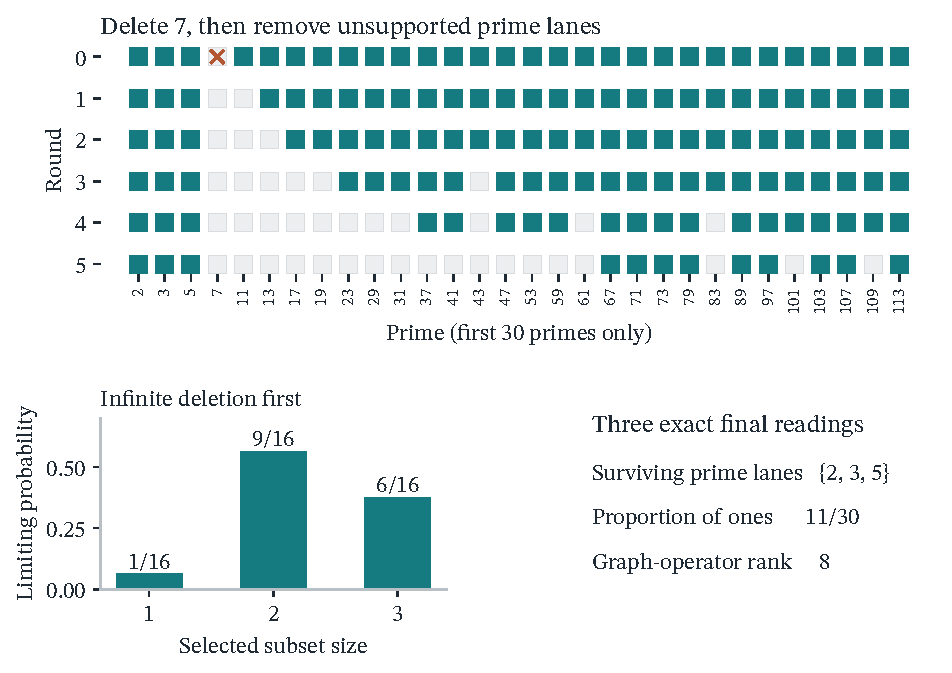
\includegraphics[width=.96\linewidth]{figures/03_delete_seven.pdf}
\caption{The upper panel follows the exact permanent-deletion rule for the first thirty primes; it is not evidence for the infinite density assertion. The lower bars give the limiting sizes of a uniformly chosen coprime subset of the $\{2,3,5\}$-smooth integers in $[2,X]$, as $X\to\infty$ after infinite deletion. The integer 1 is excluded.}
\label{fig:deletion}
\end{figure}

\subsection{An infinite spectrum becomes eight numbers}
For the last reading, give every graph vertex an independent prime
profile $\omega=(\omega_p)_{p\in\mathcal P}$: it carries $p$, meaning
$\omega_p=1$, with probability $1/p$.
Join two vertices when they share no prime in the retained set $B$.
The graph kernel and its integral operator are
\[
 G_B(\omega,\omega')=\prod_{p\in B}(1-\omega_p\omega'_p),
 \qquad
 (T_Bu)(\omega)=\int G_B(\omega,\omega')u(\omega')\,d\Prob(\omega').
\]
This operator records the graph's spectral patterns.
It is self-adjoint and Hilbert--Schmidt, and it has eigenvalues of both
signs.  It is distinct from the positive mask operator $A_g$ used in
the RH criterion.

With only $2,3,5$ retained, a vertex has eight possible relevant
profiles:
\[
 (\omega_2,\omega_3,\omega_5)\in\{0,1\}^3.
\]
Nothing else in its prime profile can affect an edge.
The final graph therefore has a finite matrix description with eight
types.  Each of the three local two-state matrices is invertible,
so all eight dimensions really occur.

Every finite round has a very different spectrum.
Let $N_{k,+}(u)$ and $N_{k,-}(u)$ count its positive and negative
eigenvalues of magnitude at least $u$.
Lemma~\ref{fin:weyl} proves
\[
 N_{k,+}(u)\sim N_{k,-}(u)\sim\frac{A_k}{2u}
 \qquad(u\downarrow0).
\]
Here $A_k>0$ measures the supply of small spectral values.
Write $K_B(4)$ for the probability that four independent profiles
form a clique when the retained restrictions are $B$.
\begin{theorem}[Infinite spectra at every finite depth]\label{fin:collapse}
Let $T_k=T_{B_k}$.  At each fixed finite depth it has infinitely many
positive and negative eigenvalues.  Their counting coefficient $A_k$
from Lemma~\ref{fin:weyl} decreases to zero.
Nevertheless $T_k$ converges in Hilbert--Schmidt norm to an operator
with exactly eight nonzero eigenvalues.  At the same time
\[
 K_{B_k}(4)\uparrow K_{\{2,3,5\}}(4)=\frac{512}{3375}.
\]
\end{theorem}

Removing prime restrictions makes such a clique more
likely, so its probability rises to $512/3375$.
At the same time $A_k$ tends to zero and the infinite spectral tail
disappears.  A fixed four-vertex experiment and the full spectrum see
different aspects of the same changing graph.

The exact tensor spectrum, the small-eigenvalue estimate, and the norm
convergence are proved in Appendix~\ref{finapp:spectrum}.
The full-prime tensor formula is due to Zagier
\cite[Appendix C]{finCoprimeChain}; here it is applied along the deletion
process.

\subsection{The initial edit can be arbitrarily late}
Deleting $7$ made the cascade easy to watch.
One can also begin arbitrarily far out in the original constant.

Let $S=\{p_i:2(i+1)\text{ has a Goldbach representation}\}$.
Choose $J\ge4$, put $r=p_J$, and initially delete the finite block
\[
 \{p_i:J<i<r\}.
\]
The same robust argument leaves density one at each finite round.
For $i\ge r$, the target $2(i+1)>2r$ cannot be made from the first
$J$ primes.  Backward dependence therefore leaves an eventual set
contained in $\{p_1,\ldots,p_J\}$.
For example, $J=4$ deletes $11$ and $13$ and leaves exactly $2,3,5,7$.

The edited lanes begin at position $p_{J+1}$.
Consequently the initial real number changes by at most
$2^{1-p_{J+1}}$.
An arbitrarily small change to the starting number can lead, under
this explicit repeated rule, to a finite eventual prime supply.

We began by hiding arithmetic answers in prime lanes.
We have now read those lanes as digits, choices and spectra.
After deleting $7$ and waiting forever, the three readings are
\[
 \frac{11}{30},\qquad \frac1{16}(1,9,6),\qquad 8.
\]
At every finite round, almost every sufficiently large prime remains.
The endpoint becomes visible only when we change the order of the
two limits.

\section{Random digits, complex heights and echoes}
\label{play:section}

The same constructions behave differently under three familiar tests.
Binary normality asks for every finite word; complex value distribution
asks which heights a curve reaches; Fourier decay asks whether a
measure forgets high frequencies.  The next observations connect those
tests to arithmetic already built into our objects.

\subsection{What would genuinely random digits mean?}

The original constant began by repeating Goldbach answers.  If every
answer is yes, its digits become $(1-\lambda(n))/2$.  It is tempting
to call these digits random.  Ordinary normality gives that word a
precise meaning: every binary word of length $k$ must occur with
frequency $2^{-k}$, for every $k$.

The relevant classical assertion is the ordinary, naturally averaged
Chowla conjecture for the Liouville function.  In its sign-pattern
form it predicts precisely these frequencies; see
\cite[Conjecture 1.3]{playMatomakiRadziwillTao2015}.  Its correlation
form says that for every nonempty finite set $J$ of distinct
nonnegative integers,
\begin{equation}
 \frac1N\sum_{n\le N}\prod_{j\in J}\lambda(n+j)
 \longrightarrow0.
 \label{play:chowla}
\end{equation}
In particular, this is a fixed-step assertion.  Averaging over the
step in the sampling theorem does not establish it.

\begin{proposition}\label{play:normality}
The original Goldbach constant is normal in base two if and only if
Goldbach's conjecture and the Liouville Chowla conjecture
\eqref{play:chowla} both hold.
\end{proposition}
\begin{proof}
Normality implies simple normality, which already implies Goldbach
by Theorem~\ref{fnd:balance}.  Under Goldbach the digit at $n$ is
$(1-\lambda(n))/2$.  For a word $w=(w_0,\ldots,w_{k-1})$, its
indicator at $n$ is
\[
 2^{-k}\prod_{j=0}^{k-1}
       \bigl(1+(-1)^{w_j}\lambda(n+j)\bigr).
\]
Expanding this product shows that \eqref{play:chowla} gives the
frequency $2^{-k}$.  Conversely, uniform frequencies of all words
give zero average to every nonconstant product of their signs.
Every finite $J$ lies inside a consecutive block, so this recovers
\eqref{play:chowla}.
\end{proof}

This equivalence helps locate the difficulty.  Normality of this one
real number simultaneously asks that no Goldbach answer be missing
and that every finite pattern of Liouville signs have its expected
frequency.  It is a meeting point of two existing conjectures, rather
than a newly available shortcut to either one.  The primitive
sampling theorem supplies a useful contrast: its fair-bit law is
unconditional because it averages over an additional variable.


\subsection{Every complex height returns}

On the real line our prime density is a positive decreasing curve.
Away from that line, its entire continuation behaves very differently.
Put
\[
 m=f(0)=\frac1{2\mathfrak C_2}.
\]
The reflection law $f(z)+f(-z)=2m$ has a surprisingly strong
consequence when combined with Picard's theorem.

\begin{proposition}\label{play:picard}
For every $a\in\mathbb C$ other than possibly $m$, the equation
$f(z)=a$ has infinitely many solutions.  In particular $f$ has
infinitely many complex zeros, but none on the real or imaginary
axis.
\end{proposition}
\begin{proof}
The nonzero coefficients at every prime position show that $f$ is
transcendental entire.  Picard's theorem says that such a function
can have at most one complex value with only finitely many
preimages \cite[Chapter II, Section 9]{playPicard1880}.  Reflection
pairs the solutions of $f(z)=a$ with those of $f(z)=2m-a$.
If $a$ had only finitely many preimages, so would $2m-a$;
hence these values must coincide, giving $a=m$.

The real-axis limits and monotonicity in
Corollary~\ref{fnd:reflection} imply $0\le f(x)\le2m$ there.
Equality at either endpoint would make $f$ constant on a real
half-line, hence constant everywhere by the identity theorem.
Thus $0<f(x)<2m$ for every real $x$.  Finally the Taylor
coefficients are real, so
$f(-iy)=\overline{f(iy)}$.  Reflection therefore gives
$\Re f(iy)=m>0$, excluding imaginary-axis zeros as well.
\end{proof}

The conclusion uses a classical theorem, but it sharpens the picture
of this particular density: a curve positive everywhere on the real
line has infinitely many zeros off both coordinate axes.  Exactly
one height escapes the argument, its central height $m$.

Reflection alone cannot settle the middle height: an odd entire
function can have only one zero.  We initially approached it as a
question about how the prime gaps constrain an entire function.
But a simpler feature of the primes settles it, and more: the only
prime divisible by $3$ is $3$.  Among the exponents $p-2$, therefore,
only the exponent $1$ is congruent to $1$ modulo $3$.  With
$\omega=e^{2\pi i/3}$, rotating the argument through three equally
spaced angles and taking a weighted sum gives
\[
 f(z)+\omega^2 f(\omega z)+\omega f(\omega^2z)
   =\frac{3z}{K'(-2)}.
\]
Every term except the linear one cancels.  This finite identity
contains information that the size of the prime gaps alone misses.
Using larger primes in the same way gives the following conclusion.

\begin{theorem}[Every polynomial target is met infinitely often]
\label{play:midpoint}
For every polynomial $P\in\mathbb C[z]$, the equation
\[
 f(z)=P(z)
\]
has infinitely many distinct solutions in $\mathbb C$.
In particular every complex value, including the middle height
$m=f(0)$, is attained infinitely often.
\end{theorem}
\begin{proof}
Choose an odd prime $q>\deg P+2$; when $P=0$, any odd prime will
do.  Put $\zeta=e^{2\pi i/q}$ and $h=f-P$.
The root-of-unity filter gives
\begin{equation}
 \sum_{j=0}^{q-1}\zeta^{-j(q-2)}h(\zeta^jz)
    =\frac{qz^{q-2}}{K'(1-q)}.
 \label{play:prime-filter}
\end{equation}
Indeed, the weighted sum kills a monomial $z^n$ unless
$n\equiv q-2\pmod q$.  It kills all of $P$, while a surviving
exponent $p-2$ of $f$ would require $q\mid p$, hence $p=q$.
The coefficient on the right is nonzero because the zero of $K$
at $1-q$ is simple.

Suppose $h$ had finitely many zeros.  Factoring them out, with
multiplicity, gives $h=D e^H$, where $D$ is a nonzero polynomial
and $H$ is entire: the remaining zero-free entire function has an
entire logarithm.  The function $H$ is nonconstant, since $h$ is
transcendental.  Substitution into \eqref{play:prime-filter} gives
a polynomial-coefficient relation among
\[
 e^{H(z)},\ e^{H(\zeta z)},\ldots,
 e^{H(\zeta^{q-1}z)},\ e^0.
\]
Narasimhan's theorem says that exponentials of entire functions
whose pairwise differences are nonconstant are linearly independent
over $\mathbb C[z]$ \cite[Theorem 1]{playNarasimhan1971}.
To apply it, group the rotated exponents whenever their difference
is constant, absorbing the corresponding constant exponential
factors into their polynomial coefficients.  Discard any group
whose combined coefficient vanishes.  The exponent $0$ remains
in its own group, since every $H(\zeta^jz)$ is nonconstant.  Its
coefficient is $-qz^{q-2}/K'(1-q)$, which is nonzero.
The resulting relation contradicts Narasimhan's theorem.
\end{proof}

Thus the bounded real curve does more than revisit every complex
height.  It meets every prescribed polynomial target infinitely
often.  The proof uses a classical independence theorem; its
arithmetic input is the elementary fact that the only prime divisible
by a prime $q$ is $q$ itself. No estimate for the distribution of primes is
needed in this step.

There is a small geometric consequence of the same cancellation.
Every complex height occurs infinitely often, yet it cannot occur
at all three vertices of an equilateral triangle centred at the
origin.  More generally, no nondegenerate regular polygon with an
odd prime number $q$ of vertices, centred at the origin, has all its
vertices at one height of $f$.  Indeed, if $f(\zeta^jz)=a$ for
every $j$ and $z\ne0$, the left side of
\eqref{play:prime-filter}, with $P=a$, is zero and the right side
is not.

The infinitude conclusion also survives any number of derivatives:
for every integer $r\ge0$ and every polynomial $P$, the equation
$f^{(r)}(z)=P(z)$ has infinitely many solutions.  The same proof
chooses a prime $q>\deg P+r+2$ and filters the exponent
$q-2-r$, whose coefficient is
$(q-2)!/((q-2-r)!K'(1-q))\ne0$; for $P=0$, take any
$q>r+2$.

There is nevertheless a useful connection with the gap-series
literature.  Erd\H{o}s recorded a conjecture of Fej\'er and P\'olya
that every entire series $\sum_k a_kz^{n_k}$ with all $a_k\ne0$
and $n_k/k\to\infty$ attains every complex value infinitely
often \cite[Section IV.8, p.~250]{playErdos1961}.
For $f-m$ the exponents are $n_k=p_{k+1}-2\sim k\log k$.
The stronger summability condition $\sum_k1/n_k<\infty$ in the
proved Fej\'er-gap theorem does not hold here
\cite[Section 1]{playMurai1983}.
Our conclusion uses the extra residue-class structure of these
particular exponents; it makes no assertion about the general
Fej\'er--P\'olya conjecture.

Before finding this argument, we explored the middle height
numerically.  Truncate the Euler product defining $K$
at primes at most $Q$, call it $K_Q$, and use the odd polynomial
\[
 P_Q(z)=\sum_{3\le p\le251}\frac{z^{p-2}}{K_Q'(1-p)}.
\]
Numerical root finding gives the following nonzero roots in the
first quadrant.
\begin{center}
\begin{tabular}{rc}
\toprule
Euler cutoff $Q$ & Root of $P_Q$, rounded\tabularnewline
\midrule
$2\,000$  & $4.202432+3.410403\,i$\tabularnewline
$8\,000$  & $4.200425+3.410428\,i$\tabularnewline
$32\,000$ & $4.199995+3.410432\,i$\tabularnewline
\bottomrule
\end{tabular}
\end{center}
At each fixed Euler cutoff, replacing the Taylor cutoff $251$ by
$149$ leaves the displayed digits unchanged.  These are roots of
finite approximations, not certified roots of $f-m$; no bound on
the remaining Euler-product error is included.  The theorem now
proves infinitely many roots without locating them.  Their positions
and rate of accumulation are taken up in
Question~\ref{play:midpoint-geometry}.

The origin is the only real solution: a nonconstant analytic
function that is nonincreasing on the real line cannot take the
same value at two distinct real points.  Oddness of $f-m$ and its
real coefficients put every root off the axes into a quartet
$z,-z,\overline z,-\overline z$.  The infinitude theorem alone
does not determine how many roots belong to such quartets.

\subsection{A full-dimensional staircase that keeps an echo}

The primitive sampling law provides another small surprise.  Its
distribution function may be singular, strictly increasing and
supported on an interval.  Yet a frequency present in that measure
reappears unchanged at every doubling of its pitch.

\begin{proposition}[Dyadic echoes]\label{play:echoes}
Under the hypotheses of Theorem~\ref{samp:staircase}, the measure
$\nu_g$ is invariant under $T(y)=2y\pmod1$.  If any lane is
disabled, its Fourier transform does not tend to zero at infinity.
More precisely, with
\[
 \widehat\nu_g(t)=\int_0^1e^{2\pi ity}\,d\nu_g(y),
\]
there is an integer $k\ne0$ such that
$\widehat\nu_g(2^jk)=\widehat\nu_g(k)\ne0$ for every $j\ge0$.
\end{proposition}
\begin{proof}
In the sampling model \eqref{samp:model}, deleting the first
binary digit replaces $(U,V)$ by $(U+V,V)$ and shifts the sequence
of fair bits.  At every prime the map $(U,V)\mapsto(U+V,V)$
permutes the nonzero residue pairs; it preserves their uniform
distribution and their independence between primes.  The shifted
fair bits have the same independent law.  This proves invariance.
The binary expansion ambiguity has measure zero because $\nu_g$
is nonatomic.

Invariance gives $\widehat\nu_g(2k)=\widehat\nu_g(k)$ for
integer $k$.  If all coefficients with $k\ne0$ vanished, integration
against every trigonometric polynomial would agree with Lebesgue
measure.  Their density among continuous functions on the circle
would force $\nu_g=\mathrm{Leb}$.  This is impossible when a lane
is disabled, because \eqref{samp:decomposition} then has a
nonzero singular part.  Choose a nonzero coefficient and iterate.
\end{proof}

In particular, the explicit singular law from
\eqref{samp:explicit-mask} has Hausdorff dimension one but no
Fourier decay along an infinite sequence.  Its Fourier dimension
is zero.  The mechanism is the familiar one for a nonuniform
dilation-invariant measure; the sampling construction supplies a
specific arithmetic instance.

There is also more than one way for dimension to vary inside a
single sampling law.  As a small exact example, disable only the
lane of $3$.  Depending on the residues of the step $V$, the
proportion of free bits takes three values:
\begin{center}
\begin{tabular}{lcc}
\toprule
Condition on the primitive step & Probability & Free-bit proportion\tabularnewline
\midrule
$3\mid V$ & $1/4$ & $1$\tabularnewline
$3\nmid V,\ 2\nmid V$ & $1/2$ & $5/6$\tabularnewline
$3\nmid V,\ 2\mid V$ & $1/4$ & $2/3$\tabularnewline
\bottomrule
\end{tabular}
\end{center}
Indeed, $\Prob(p\mid V)=1/(p+1)$ independently at distinct
primes.  If $3\mid V$, the disabled lane is avoided.  If $V$ is
odd and not divisible by $3$, exactly one index in every six has
least prime factor $3$.  If $V$ is even and not divisible by $3$,
primitivity forces all progression values to be odd, and one index
in every three is closed.

For a fixed one of these periodic patterns, every compatible
$n$-digit cylinder has probability $2^{-dn+O(1)}$, where $d$ is
its free-bit proportion.  Distinct patterns having incompatible
forced-zero sets are almost surely eventually distinguished by
their fair bits.  In the finite mixture, compatible patterns with
larger $d$ contribute exponentially less.  Consequently the
dyadic local dimension of this law is $1$, $5/6$ or $2/3$ with
the respective probabilities in the table.  Here dyadic local
dimension means
\[
 d_\nu(y)=\lim_{n\to\infty}
      \frac{-\log_2\nu(I_n(y))}{n},
\]
when the limit exists, where $I_n(y)$ is the dyadic interval of
length $2^{-n}$ containing $y$.  This example shows why the
full-dimension statement in the sampling theorem does not assert
one local dimension almost everywhere.

The three values give an exact starting point for the infinite-mask
problem in Question~\ref{play:local-dimensions}.  The geometry already
varies inside one law, independently of which Goldbach answers occur.

\clearpage
\section{Conjectures and open questions}\label{open:section}

The proved statements leave a small set of next steps.  We distinguish
the one prediction stated as a conjecture from six questions whose
answers are not established here.  The definitions are recalled so
that each can be read independently.  The connection to classical
conjectures remains visible in Proposition~\ref{play:normality}:
normality of the original constant is equivalent to Goldbach together
with the naturally averaged Liouville Chowla conjecture.

\subsection{A conjecture about the typical deletion time}

In the deletion experiment of Section~\ref{fin:deletion}, begin with
all primes except $7$.  At every round retain $p_i$ only when
$2(i+1)$ is the sum of two currently retained primes; the same
prime may be used twice, and all deletions happen simultaneously.
Write $\tau(p)$ for the first round in which $p$ is absent, with
$\tau(7)=0$ and $\tau(2)=\tau(3)=\tau(5)=\infty$, and put
\[
 M(x)=\max_{5<p\le x}\tau(p),
\]
where the maximum is over primes.  Proposition~\ref{fin:depthclock}
proves $M(x)\sim\log x/\log\log x$.  This is the clock of the
last survivor in a finite window.  We conjecture that it also gives
the typical deletion time.

\begin{conjecture}[Most primes share the last survivor's clock]\label{fin:typicaldepth}
Let $P_x$ be a uniformly chosen prime in $(5,x]$.
Then
\[
 \frac{\tau(P_x)}{M(x)}\longrightarrow1
 \qquad\text{in probability}.
\]
\end{conjecture}

Here the randomness is only the uniform choice of $P_x$; the deletion
process itself is deterministic.  The exact computation through
$10^6$ found that about $94.1\%$ of the $78\,495$ primes above $5$
disappear in rounds $11$, $12$ or $13$, with $M(10^6)=13$.
The proposition proves the clock for the last surviving prime.
The conjecture asks whether nearly the whole population follows it.
The computation is a finite experiment, not evidence for a specific
error term; fixed-depth abundance alone does not settle this question.

\subsection{How much data does arithmetic recovery need?}

Both questions in this subsection use the ordinary-integer experiment
of \eqref{rec:finite-model}.  There are $N$ labelled boxes, with hidden
contents $X_1,\ldots,X_N$ independently uniform on
$\{1,\ldots,N^2\}$.  For each unordered pair we observe one bit saying
whether the contents are coprime, independently flipped with common
probability $\varepsilon_N$.  The flips are independent of the
integers; the decoder is not told $\varepsilon_N$.
Theorem~\ref{rec:threshold} identifies the consistency threshold
\[
 T_N=N(1-2\varepsilon_N)^2\longrightarrow\infty.
\]
It names the shared primes on a fraction of pairs tending to one.
Corollary~\ref{rec:profiles} then recovers divisibility by each fixed
prime at a fixed labelled box.  These are asymptotic results; the
following asks for a useful finite guarantee.  Take $N^2\ge p$ so
that conditioning on either divisibility outcome is meaningful.

\begin{question}[How many boxes are needed to name a prime?]\label{rec:prime-sample-question}
In the finite experiment, fix a prime $p$, a constant edge-flip rate
$\varepsilon_N=\varepsilon\ne1/2$, and
$0<\delta<1/2$. How large must $N$ be to decide whether $p\mid X_i$,
with conditional error at most $\delta$ both for a multiple and for a
nonmultiple of $p$? Require a computationally feasible procedure that
is not supplied the error rate. How does the answer grow with $p$
and with the closeness of the channel to a fair coin?
\end{question}

The second question concerns the original message rather than the
full collection of shared-prime sets.  Fix an unknown mask
$g=(g_j)$ with $g_1=1$, and set
\[
 x_g(1)=0,\qquad
 x_g(n)=\frac{1-\lambda(n)}2g_{\ell(n)}\quad(n\ge2),
\]
where $\ell(n)$ is the index of the least prime factor of $n$.
Alongside the noisy graph, observe aligned digit marks
\[
 Z_i=x_g(X_i)\mathbin{\oplus}B_i',
 \qquad B_i'\sim\operatorname{Bernoulli}(\eta_N).
\]
These digit flips are independent of one another, the integers and
the edge flips.  As in Theorem~\ref{rec:message}, the digit-noise
probability $\eta_N$ is supplied; the edge-noise probability is not.
Writing $a_N=1-2\varepsilon_N$ and $b_N=1-2\eta_N$, that theorem
recovers both the message and almost every shared-prime set when
$Na_N^2\to\infty$ and $Nb_N^2\to\infty$.
Here recovering the message means recovering each fixed finite prefix
of $g$ with probability tending to one as $N$ grows.

\begin{question}[How much graph does the message need?]\label{rec:message-only-question}
If the only required output is the arithmetic message, what conditions
on the two noise sequences suffice? In particular, can the edge signal
be weaker than the threshold needed to recover shared-prime sets?
\end{question}

This asks for a separate decoding theorem.  The joint-task result
supplies the digit-noise rate to the procedure, and makes no assertion
of adaptation to an arbitrary unknown rate approaching one half.

\subsection{Can one hear every disabled prime?}

The exact bias can confuse a single disabled lane with infinitely
many of them, as Proposition~\ref{grw:bias-collision} shows.  The
whole function distinguishes that example immediately: one function
is linear and the other is transcendental.  How much farther does
this recovery go?

For this question only, write $\Phi_{\mathcal F}$ for the normalized
entire function in \eqref{fnd:two-functions} whose disabled-prime set
is $\mathcal F$.  Its Taylor coefficients are $M_k/k!$, where $M_k$
are the conditional correlations of Section~\ref{fnd:correlations}.
The counting exponent of
$\mathcal F$ is
\[
 \limsup_{R\to\infty}
 \frac{\log\max(1,\#(\mathcal F\cap[2,R]))}{\log R}.
\]
Restrict to masks with counting exponent strictly below one, so that
their zero multisets determine the normalized entire functions by
Corollary~\ref{grw:zeros}.

\begin{question}[Hearing the mask]\label{play:mask-rigidity}
Let $\mathcal F$ and $\mathcal H$ be sets of odd primes whose
counting exponents are strictly below one.  Does
\[
 \Phi_{\mathcal F}\equiv\Phi_{\mathcal H}
 \quad\Longrightarrow\quad \mathcal F=\mathcal H?
\]
Equivalently, can two different such masks have exactly the same
complex zeros, including multiplicities?
\end{question}

There are three equivalent ways to supply the data: all conditional
correlations $M_k$, the entire function $\Phi$, or the nonzero
eigenvalues of the positive mask operator $A_g$.  Indeed,
$\Psi$ is obtained from $\Phi$ by multiplying its $k$th Taylor
coefficient by the fixed nonzero number $K(k)$, and
$\Psi(z)=\prod_j(1+\alpha_jz)$ records those eigenvalues.
Thus this is also an inverse spectral question for a restricted
arithmetic family of operators.

For finite masks the answer is yes: even the first derivative
$\Phi'(0)=S_g$ determines the mask.  An infinite mask cannot agree
with a finite one because the corresponding functions have different
degrees.  A possible failure must therefore involve two infinite
masks.  We already know that identical functions would force the
same counting exponent.  The question is whether the higher
correlations retain the individual prime locations as well.

\subsection{Does the triangular match include the last root?}

Recall
\[
 J_N(z)=\sum_{k=0}^N\binom Nk K(k)z^k,
\]
where $K(k)$ is the limiting probability that $k$ random integers
are pairwise coprime.  Its roots are negative; write them as
$-R_{N,1},\ldots,-R_{N,N}$, with $R_{N,j}>0$ and multiplicities
included.  Theorem~\ref{tri:main} shows that the empirical
distribution of
\[
 \frac{\exp(e^{-\gamma}R_{N,j})}{N\log N}
\]
approaches the Dykema--Haagerup law $\operatorname{DH}_1$, whose
support is $[0,e]$; $\gamma$ is Euler's constant.  This is a
statement about the whole histogram.

\begin{question}[Does the last root find the same edge?]\label{tri:edgequestion}
Do the largest arithmetic roots satisfy
\[
 e^{-\gamma}\max_jR_{N,j}-\log N-\log\log N\longrightarrow1,
\]
or, equivalently,
\[
 \max_j\frac{\exp(e^{-\gamma}R_{N,j})}{N\log N}
 \longrightarrow e?
\]
\end{question}

This asks whether the match reaches the edge as well as the histogram.
For the Gaussian triangular matrix, the largest squared singular value
does tend to $e$ \cite[Theorem 2]{triCheliotis}.
The empirical convergence proved here leaves room for a small number
of arithmetic outliers.  It implies the corresponding lower limit is
at least $e$, since the limiting law has mass arbitrarily close to that
edge; excluding larger outliers needs more.
The same distinction leaves convergence of transformed empirical
moments unproved.

\subsection{Locating the returns to the middle height}

Let $f$ be the entire prime density of
Theorem~\ref{fnd:entire-density}, and set
$m=f(0)=1/(2\mathfrak C_2)$.
Theorem~\ref{play:midpoint} proves that every polynomial target is
met infinitely often.  For the target $m$, the origin is the only
real solution; reflection and conjugation place roots off the axes
in quartets.  The theorem does not locate those roots.

\begin{question}[Where does the middle height return?]
\label{play:midpoint-geometry}
Are there infinitely many solutions of $f(z)=m$ on the imaginary
axis?  How fast does
\[
 N_m(R)=\#\{z\in\mathbb C:|z|\le R,\ f(z)=m\},
\]
with multiplicities counted, grow as $R\to\infty$?
\end{question}

The first-quadrant calculation in Section~\ref{play:section} is an
experiment with finite approximations, not a certification of a root.
The imaginary-axis question asks about a different part of the
geometry, while the counting question measures how often the middle
height returns in the whole plane.

\subsection{The dimensions inside a singular staircase}

Let $p_j$ be the $j$th prime.  Disable exactly the lanes in
$\mathcal F_*=\{p_{2^j}:j\ge2\}$, the explicit mask
\eqref{samp:explicit-mask}, and write $\nu_*$ for its primitive
sampling measure from Theorem~\ref{samp:staircase}.  This measure is
singular continuous, has support $[0,1]$, and has Hausdorff dimension
one.  The local dimension describes a different feature: how quickly
the probability around an individual point shrinks.

For $y\in[0,1]$, let $I_n(y)$ be its dyadic interval of length
$2^{-n}$; endpoints may be assigned consistently to either adjacent
interval since the measure is nonatomic.  Choose $Y$ with law
$\nu_*$.  Then the following local dimension is itself a random
variable.

\begin{question}[The dimensions inside the staircase]
\label{play:local-dimensions}
For the explicit infinite mask
$\mathcal F_* =\{p_{2^j}:j\ge2\}$, determine the distribution of
\[
 \underline d_*(Y)=\liminf_{n\to\infty}
       \frac{-\log_2\nu_*(I_n(Y))}{n},\qquad Y\sim\nu_*.
\]
In particular, does this distribution have any atoms?
\end{question}

The example with only the lane of $3$ disabled, in
Section~\ref{play:section}, gives an exact comparison: its local
dimension equals $1$, $5/6$ or $2/3$, with probabilities $1/4$,
$1/2$ and $1/4$.  Infinitely many prime lanes may produce a richer
distribution than these three values.  The question concerns the
geometry of the construction independently of which Goldbach
answers occur.

\clearpage
\section{Back to the constant}\label{end:visible}

The first construction fitted a list of arithmetic questions into one
real number. Each prime carried a question; its lane repeated the answer.
That repetition let a single missing answer alter a limiting percentage,
break a self-similarity, and turn Euler's convergent sum into infinity.

Reading the positions through coprimality changed the questions we could
ask. Correlations counted missing lanes. Their generating functions
turned that count into degrees, zeros and spectral directions. A random
scale connected two ways of averaging, and its density became the curve
whose derivatives recognize primes. The prime and composite parts could
even be put back together to recover an ordinary exponential law.

Then we hid the numbers. The relationships still revealed prime names.
The cancellation of three observed frequencies explained why; the noisy
experiment quantified how far the idea could go. Its paradox survives
the precise rules of the game: the exact shared primes of a fraction of
pairs tending to one can be recovered while the retained fraction of
information about the complete table tends to zero. The surviving
information grows, but the uncertainty about the whole table grows
faster. Both facts belong in the picture.

The later experiments asked what arithmetic arrangements look like.
Coprime crowds could leave earlier holes in the list of covered primes.
Averaging a matrix and averaging its characteristic polynomial revealed
different spectra. Conditioning a factorization to be unusually balanced
produced a Gaussian profile. These conclusions make sense on their own;
the shared constructions gave us a route from one question to the next.

Finally we returned to the original assignment and removed seven.
Almost all primes survived every fixed number of rounds. Only three
survived forever. The same arithmetic could appear abundant or almost
empty, depending on when we looked.

A last change of view sent the curve into the complex plane. Its prime
coefficients made it meet every polynomial infinitely often, yet prevented
any three points with the same value from forming an equilateral triangle
centred at the origin. A rotation that keeps just one prime explained both
conclusions.

Section~\ref{open:section} gathers the conjecture and questions left
by these experiments: their hidden messages, complex values, spectra
and long-term behavior.  The earlier connections to classical
arithmetic questions also remain invitations to further work.
Goldbach, RH and twin primes remain open, and a new formulation
needs new input before it can settle them.

The unifying question is simpler: what can a number remember after we
change the way we observe it? Here it remembered arithmetic in a digit
frequency, in a curve's missing derivatives, in the signs of a matrix,
and in noisy relationships between closed boxes. Each observation
revealed something the previous one had made difficult to see.

\clearpage
\appendix
\small
\section{Proofs behind the constant and the curve}\label{app:foundations}

The main text keeps the elementary digit arguments beside their conclusions. This appendix supplies the longer operator and density arguments.

\subsection{The finite part of the heat trace}\label{app:fnd:heat-binary}

\begin{proof}[Proof of Proposition~\ref{fnd:heat-binary}]
Summing a Dirichlet series on one least-prime lane gives
\begin{align*}
 \sum_{\ell(n)=j}n^{-s}
 &=p_j^{-s}\zeta(s)\prod_{r<j}(1-p_r^{-s}),\\
 \sum_{\ell(n)=j}\lambda(n)n^{-s}
 &=-p_j^{-s}\frac{\zeta(2s)}{\zeta(s)}
     \prod_{r<j}(1+p_r^{-s}).
\end{align*}
Initially for $\Re s>1$, convolution with the constant-one
function therefore gives
\begin{equation}
 Z_{\Gold}(s):=\sum_{m\ge1}c_mm^{-s}
 =\zeta(2s)(1+C(s))+\zeta(s)^2A(s).
 \label{fnd:spectral-zeta}
\end{equation}
This identity supplies meromorphic continuation.  Mellin inversion
of the exponential, followed by a contour shift from $\Re s>1$
to $\Re s=-1/2$, gives
\[
 \Theta_{\Gold}(t)=1+\frac2{2\pi i}\int
 \Gamma(s)Z_{\Gold}(s)(\pi t)^{-s}\,ds
\]
with residues at $1,1/2,0$.  The finite Dirichlet polynomials are
bounded on each vertical line, zeta has polynomial growth there,
and gamma decays exponentially.  The shifted integral is therefore
$O_F(\sqrt t)$; these are the standard Mellin contour estimates
in \cite[Section 2.5]{fndDLMF}.

At $s=1$, the double pole of $\zeta(s)^2A(s)$, together with
$\Gamma'(1)=-\gamma$, gives the first line of
\eqref{fnd:heat-binary-expansion}.  The residue of $\zeta(2s)$
at $1/2$ gives its second divergent term.  Finally $C(0)=B$,
$A(0)=0$ because the lane of $2$ is enabled, and
$\zeta(0)=-1/2$.  Hence $Z_{\Gold}(0)=-(1+B)/2$.
The residue at zero and the separate zero-energy state combine
to give $1+2Z_{\Gold}(0)=-B$.
\end{proof}

\subsection{A positive operator for the message}\label{app:fnd:mask-operator}

Let $\mathcal F=\{p_j:g_j=0\}$ and $D=z\,d/dz$.
For a prime cutoff $R$, start with $U=1$ and apply successively
\begin{equation}
 U\longleftarrow(D+p-1+\mathbf1_{\{p\in\mathcal F\}}z)U,
 \qquad p\le R.
 \label{fnd:prime-operator}
\end{equation}
Call the result $U_R$.  For the mask in which only
$\mathcal F\cap[2,R]$ is disabled, denote the first function in
\eqref{fnd:two-functions} by $\Phi_{g,R}$.  Then
\begin{equation}
 [z^k]\Phi_{g,R}(z)=
 \frac{[z^k]U_R(z)}{\prod_{p\le R}(p+k-1)}.
 \label{fnd:operator-coefficients}
\end{equation}
Indeed, let $v_j$ be the probability that exactly $j$ coordinates
have received a first label, all such labels were disabled, and no
coordinate has received a successful first label.  At prime $p$,
\[
 v_j^{\rm new}=
 \frac{(p+j-1)v_j+
 \mathbf1_{\{p\in\mathcal F\}}(k-j+1)v_{j-1}}{p+k-1}.
\]
Divide $v_j$ by the falling factorial $(k)_j$ and clear the common
denominators.  This is exactly the coefficient recurrence in
\eqref{fnd:prime-operator}.  At $j=k$, the probability is
$M_k(g,R)$, proving \eqref{fnd:operator-coefficients}.

The all-active form of this differential recurrence is a generalized
Bell-polynomial recurrence studied in \cite{fndDuran2024}.  We give
the masked normalization and positive construction explicitly,
because they are what connect the recurrence to the digits.



\begin{proof}[Proof of Theorem~\ref{fnd:mask-operator}]
Set
\[
 \eta_R=\prod_{p\le R}\frac{p-1}{p},\qquad
 \mathcal P_R(z)=\frac{U_R(\eta_Rz)}{\prod_{p\le R}(p-1)}.
\]
Its constant term is one.  If
$K_R(k)=\prod_{p\le R}(1-1/p)^k(1+k/(p-1))$, then
\eqref{fnd:operator-coefficients} gives
\begin{equation}
 [z^k]\mathcal P_R(z)=K_R(k)\frac{M_k(g,R)}{k!}.
 \label{fnd:normalized-coefficients}
\end{equation}
These coefficients are between zero and $1/k!$ and tend to
$K(k)M_k(g)/k!$.  It follows that $\mathcal P_R\to\Psi_g$
locally uniformly.

We construct positive matrices with determinant $\mathcal P_R$.
Suppose the previous matrix has eigenvalues
$\alpha_1,\ldots,\alpha_m>0$.  At prime $p$, put
$c=p-1$, $u=c/p$ and $\eta_{\rm new}=u\eta_{\rm old}$.
Begin with
\[
 B=\operatorname{diag}(u\alpha_1,\ldots,u\alpha_m),\qquad
 w=(\sqrt{u\alpha_1},\ldots,\sqrt{u\alpha_m})^{\mathsf T}.
\]
If $p\in\mathcal F$, adjoin one zero coordinate to $B$ and
the component $\sqrt{\eta_{\rm new}}$ to $w$.  In either case
set $A_R=B+c^{-1}ww^{\mathsf T}$.  Start with the empty matrix.
The matrix determinant lemma gives
\[
 \det(I+zA_R)=
 \left(1+\frac Dc+
 \frac{\mathbf1_{\{p\in\mathcal F\}}\eta_{\rm new}z}{c}\right)
 \mathcal P_{<p}(uz),
\]
which is the normalization of \eqref{fnd:prime-operator}.
The matrices are positive definite whenever nonempty: a newly
adjoined null coordinate is filled by the nonzero last component
of $w$.

The old diagonal entries of $A_R$ are exactly the previous
$\alpha_i$, because $u(1+1/c)=1$.  At a disabled prime the new
diagonal entry is $\eta_{\rm old}/p=\delta_{\ell(p)}$.
Therefore
\begin{equation}
 \operatorname{tr}A_R=
 S_R:=\sum_{\substack{p\le R\\p\in\mathcal F}}\delta_{\ell(p)}
 \longrightarrow S_g.
 \label{fnd:finite-trace}
\end{equation}
Sort each eigenvalue list decreasingly and pad it with zeros.
For every fixed $j$, the sum of its first $j$ entries is
nondecreasing through the updates: the variational characterization
of that sum bounds it below by the trace on the old leading $j$
coordinate directions.  These sums are bounded by one and hence
converge.  Their consecutive differences define a decreasing
summable list $\alpha_1,\alpha_2,\ldots\ge0$.

No trace disappears in this passage.  Given a cutoff with $m$
disabled primes, every later sum of the first $m$ eigenvalues is
at least $S_R$.  Passing to the limit and then increasing the
cutoff shows $\sum_j\alpha_j\ge S_g$.  The reverse inequality
follows from \eqref{fnd:finite-trace}.  Thus the padded lists
converge in $\ell^1$, and their determinant products converge
locally uniformly to
\[
 \Psi_g(z)=\prod_j(1+\alpha_jz),\qquad \sum_j\alpha_j=S_g.
\]
Take $A_g$ to be the diagonal operator with these positive
eigenvalues.  In the finite-mask case its rank equals the degree,
which is $\#\mathcal F$ by Proposition~\ref{fnd:moment-positivity}.
In the infinite case every coefficient is positive, so the function
cannot be a finite product.  This proves the rank statement and
the location of the zeros.
\end{proof}

\subsection{Why the entire series is the actual density}\label{app:fnd:entire-density}

\begin{proof}[Proof of Theorem~\ref{fnd:entire-density}]
For a cutoff $R$, write
\[
 L_R=\prod_{p\le R}\frac p{p-1},\qquad
 Y_R=\sum_{p\le R}\frac{E_p}{p-1},\qquad
 W_R=L_Re^{-Y_R}.
\]
The summands of $Y_R$ have distinct exponential rates $r_p=p-1$.
Partial fractions of $\prod_{p\le R}r_p/(r_p+s)$ show that
the density of $Y_R$ is
\[
 \sum_{p\le R}
 r_p\prod_{\substack{q\le R\\q\ne p}}
 \frac{r_q}{r_q-r_p}\ e^{-r_py},\qquad y>0.
\]
After the change of variable $w=L_Re^{-y}$ this becomes
\begin{equation}
 f_R(w)=\sum_{p\le R}c_{p,R}w^{p-2}\quad(0<w<L_R),
 \qquad c_{p,R}=\frac1{K_R'(1-p)}.
 \label{fnd:finite-density}
\end{equation}
It is zero for $w>L_R$.  One can check the coefficient without
transform notation: the change of variable multiplies the
coefficient of $e^{-r_py}$ by $L_R^{-r_p}$, which is exactly
the reciprocal derivative in \eqref{fnd:finite-density}.

For fixed $p$, the derivative $K'(1-p)$ is nonzero.  Its factors
from primes below $p$ are negative, and all remaining factors
apart from the differentiated one are positive, proving the
claimed sign.  Moreover
\begin{equation}
 |c_{p,R}|\le |c_p|\quad(R\ge p),\qquad c_{p,R}\longrightarrow c_p.
 \label{fnd:coefficient-domination}
\end{equation}
Indeed, adding a prime $q>p$ to the derivative multiplies it by
\[
 \left(1+\frac1{q-1}\right)^{p-1}
 \left(1-\frac{p-1}{q-1}\right),
\]
a number strictly between zero and one.  Taking logarithms and
using $\log(1+u)<u$ and $\log(1-v)<-v$ proves the upper bound
of one.  The infinite tail converges to a nonzero product.

We next bound the infinite coefficient.  Put $m=p-1$.  Separating
the prime factors at $2p$ gives the exact expression
\begin{align*}
 \log|K'(-m)|={}&m\sum_{q\le2p}\log\frac q{q-1}-\log m\\
 &+\sum_{\substack{q\le2p\\q\ne p}}
       \log\frac{|q-p|}{q-1}\\
 &+\sum_{q>2p}\left[m\log\frac q{q-1}
       +\log\left(1-\frac m{q-1}\right)\right].
\end{align*}
Mertens' product estimate makes the first line
$p\log\log p+O(p)$; a statement of the classical product
estimate is recalled in \cite[Section 2]{fndLagarias2002}.
Each ratio in the middle line lies between $1/(2p)$ and $2p$.
Chebyshev's bound $\pi(2p)=O(p/\log p)$ therefore bounds
that line in absolute value by $O(p)$.
For $q>2p$, cancellation of the linear terms leaves an error
$O(p^2/q^2)$, whose sum is $O(p)$ even if all integers $q>2p$
are included.  This proves \eqref{fnd:residue-decay}.  It follows
that the series in \eqref{fnd:density-series} converges absolutely
and uniformly on every compact subset of $\mathbb C$.

Finally, $L_R\to\infty$ by Mertens' theorem.  On any fixed
interval $[0,B]$, the polynomial formula
\eqref{fnd:finite-density} therefore applies for large $R$,
with values at zero supplied by continuity.  Equations
\eqref{fnd:coefficient-domination} and
\eqref{fnd:residue-decay} imply uniform convergence $f_R\to f$
there, by dominated convergence of the power series.
On the other hand, $W_R\to W$ almost surely.  For every continuous
compactly supported test function in $(0,\infty)$, uniform
convergence of densities and weak convergence of the random
variables give the same integral.  Hence the restriction of $f$
to $(0,\infty)$ is exactly the law's density.  Since $W$ is
positive and finite almost surely, no missing mass occurs at an
endpoint.  Its integral is one.  Each $c_p$ is nonzero, proving
\eqref{fnd:prime-taylor-support}.
\end{proof}

\subsection{Why signed correlations become probabilities}\label{app:correlations}
\begin{proof}[Proof of Proposition~\ref{fnd:moment-positivity}]
Write $a_g=h_g+(1-h_g)\lambda$ as in
\eqref{fnd:mask}.  Truncate the lane mask to primes at most $R$,
and truncate the coprimality condition at the same cutoff.  The
mean error is at most a constant depending on $k$ times
\[
 \prod_{p\le R}(1-1/p)+\sum_{p>R}p^{-2}+o_N(1).
\]
The first term bounds coordinates with no prime divisor at most
$R$; the second bounds a large-prime collision.

For fixed $R$, expand the product of the truncated signed digits.
Every term containing a Liouville factor in at least one coordinate
has average zero.  To see this, partition the finite prime
divisibility patterns among coordinates.  In each coordinate,
inclusion--exclusion reduces the required sum to finitely many
expressions $\lambda(d)L(N/d)$ with fixed $d$, which are $o(N)$.
The other coordinates contribute bounded normalized sums.  Thus
only the term $\prod_i h_g(n_i)$ remains in the limit.
Letting $R\to\infty$ and dividing by the positive limit $K(k)$
proves existence and identifies the conditional moment as a
probability.

Conditioning the local independent divisibility model on at most
one divisible coordinate gives precisely the probabilities in the
statement.  Conditioning at finitely many primes preserves
independence across those primes; passage to all primes is valid
because the no-collision probability tends to $K(k)>0$.
Each coordinate receives a first prime almost surely, since
$\prod_p(1-1/(p+k-1))=0$.  The first labels are distinct.
There can therefore be no successful outcome with fewer than $k$
disabled primes.  Given $k$ such primes, prescribe them as the
first labels of the coordinates and prescribe no incompatible
choices at the finitely many earlier primes.  This event has
positive probability.  The case $k=1$ is the lane-density formula.
\end{proof}

\section{Proof of the primitive sampling theorem}
\label{samp:proofs}

This appendix proves Theorem~\ref{samp:staircase}.  The main text gave
its probabilistic mechanism; here we justify the limiting distribution,
the exact Lebesgue decomposition, and the dimension statement.

\begin{proof}
We first obtain the limiting probability model.  Take a pair of
Haar-uniform profinite integers $(U,V)$, conditioned on having no
common prime divisor.  This event has probability
$\prod_p(1-p^{-2})=6/\pi^2$.  At each prime $p$, the residues $(U,V)$
are therefore uniform among the $p^2-1$ pairs other than $(0,0)$;
these choices are independent at distinct primes.  Independently
choose fair bits $B_0,B_1,\ldots$.  The candidate limit is the law of
\begin{equation}
 Z_g=\sum_{j\ge0}\bigl(1-h_g(U+jV)\bigr)B_j2^{-j-1}.
 \label{samp:model}
\end{equation}
The least prime of each $U+jV$ exists almost surely.  For example,
under this local law
$\Prob(p\mid U+jV)=1/(p+1)$, and independence over primes shows
that the probability of avoiding every prime is zero.

For completeness, the analytic input that produces the fair bits
is the following variable-step cancellation: for any nonempty finite
$J\subset\{0,1,\ldots\}$ and any fixed function $P(a,d)$ periodic
in both variables,
\begin{equation}
 \frac1{N^2}\sum_{a,d\le N}P(a,d)
       \prod_{j\in J}\lambda(a+jd)\longrightarrow0.
 \label{samp:cancellation}
\end{equation}
Theorem~2.5 of Frantzikinakis--Host \cite{sampFrantzikinakisHost2017}
gives vanishing Gowers norms of every fixed order for the aperiodic
function $\lambda$; their Lemma~9.6 controls products on independent
linear forms.  To include $P$, expand it in its finite Fourier
series.  For $j_0\in J$ a phase $e((ra+sd)/Q)$ factors as
$e(r(a+j_0d)/Q)e((s-rj_0)d/Q)$, where $e(t)=e^{2\pi it}$.
Absorb the first factor into $\lambda(a+j_0d)$ and the second into
the additional form $d$.  Multiplication by a linear phase preserves
Gowers norms of order at least two.  Extend the first function evenly
from positive integers, as required by that lemma.  The forms
$a+jd$ and $d$ are pairwise independent, proving
\eqref{samp:cancellation}.  Thus no assertion about correlations
at a fixed step is being used.

Fix a prefix length $k$.  Truncate both the mask and the coprimality
condition at primes at most $R$.  All mask coefficients and
restrictions are now periodic in $(a,d)$.  Expand a prefix indicator
using $1-2x_g=h_g+(1-h_g)\lambda$.  Every term containing a
Liouville factor vanishes by \eqref{samp:cancellation}; the other
terms converge by the Chinese remainder theorem.  These are exactly
the prefix probabilities in \eqref{samp:model}, with the same
truncations.  The proportion of pairs missed by truncated
coprimality is at most $\sum_{p>R}p^{-2}$, since
$\lfloor N/p\rfloor^2\le N^2/p^2$.  A mask error at $a+jd$
requires that integer to avoid all primes at most $R$.  For fixed
$R$, its limiting proportion in the square is
$\prod_{p\le R}(1-1/p)$, which tends to zero.  Summing this error
over the $k$ positions and then removing both truncations proves
prefix convergence.  A continuous function of the sampled real is
uniformly approximated by a function of its first $k$ digits, since
the remaining binary tail is at most $2^{-k}$.  This proves weak
convergence to the law of $Z_g$.

Next fix a primitive profinite pair $(U,V)$.  A lane $p$ is visited
by $U+jV$, $j\ge0$, if and only if $p\nmid V$.  If $p\mid V$,
primitivity gives $p\nmid U$, so the lane is avoided.  Otherwise
prescribe the unique root modulo $p$ and avoid the roots modulo
each smaller prime $q$ with $q\nmid V$.  There is an allowed residue
at each such $q$; primes dividing $V$ already divide no term.
The Chinese remainder theorem gives an index with least prime $p$,
and the same event repeats periodically in $j$.

All digits of the progression are open precisely when $p\mid V$
for every $p\in\mathcal F$.  Locally this has probability
$(p-1)/(p^2-1)=1/(p+1)$, proving that the all-open event has
probability $L_g$.  On it, $Z_g$ is uniform on $[0,1]$.
An all-closed progression would require $p\mid V$ for every
successful prime.  There are infinitely many such primes by
\eqref{samp:success-hypothesis}, so that event has probability zero.
Almost every fiber therefore has an open lane, hence infinitely many
independent fair bits.  Its binary law is nonatomic, and so is its
image on $[0,1]$.

If a fiber has any closed position, that position repeats along an
infinite arithmetic progression of indices.  All the corresponding
bits are forced to zero.  The set of binary sequences with zeros on
some infinite arithmetic progression is a countable union of
fair-coin null sets.  Its image has Lebesgue measure zero.  Every
fiber with a closed position is carried by this same null set.
This common support, together with non-atomicity, proves the exact
decomposition \eqref{samp:decomposition}.

To prove full support, choose any $k$ distinct successful primes
$s_0,\ldots,s_{k-1}$, and take $R>\max s_j$.  At disabled primes
$q\le R$ impose $V=0$, $U\ne0$ modulo $q$.  At successful primes
$q\le R$ impose $V\ne0$; at $s_j$ also impose $U+jV=0$.
These compatible local conditions have positive probability.
They make each of the first $k$ positions open: it has a successful
prime divisor below $R$ and no disabled divisor there.
The independent fair bits can then realize any prescribed word.
Every dyadic interval has positive mass.

Finally, impose the same conditions below $R$, without prescribing
the first $k$ positions.  Call this positive-probability event $D_R$.
For any fixed local residues on $D_R$, every closed index belongs to
the periodic set avoiding the single roots at all successful
primes $q\le R$.  This set has density
\[
 \varepsilon_R=\prod_{\substack{q\le R\\q\notin\mathcal F}}(1-1/q).
\]
With $Q_R=\prod_{q\le R}q$, at least
$(1-\varepsilon_R)n-Q_R$ of the first $n$ bits are consequently
open.  The submeasure
$\mu_R(B)=\Prob(Z_g\in B,\ D_R)$ satisfies, for every dyadic
interval $I$ of length $2^{-n}$,
\[
 \mu_R(I)\le 2^{Q_R}2^{-(1-\varepsilon_R)n}.
\]
The same bound with a different constant holds for arbitrary
intervals, by covering one interval with at most two dyadic
intervals of comparable length.  Any full-$\nu_g$-measure Borel
set has positive $\mu_R$ mass.  Covering it by intervals and summing
this bound shows that its Hausdorff dimension is at least
$1-\varepsilon_R$.  Hypothesis \eqref{samp:success-hypothesis}
gives $\varepsilon_R\to0$, proving dimension one.  A nonatomic
full-support probability has a continuous strictly increasing
distribution function; differentiation of its Lebesgue
decomposition gives the final assertion.
\end{proof}

\IfFileExists{sections/phi_growth_proofs.tex}{\section{Growth estimates for the mask function}
\label{grw:proofs}

The proof of Theorem~\ref{grw:order} matches an upper bound from all
possible assignments with a lower bound from one carefully chosen set
of assignments.

\begin{proof}
For every $\eta_g<\beta<1$, $B_g(u)\ll_\beta u^\beta$;
this also ensures convergence of the reciprocal sum.  Integration
by parts in \eqref{grw:majorant} yields
\begin{equation}
 \log P_{\mathcal F}(r)
 =r\int_2^\infty\frac{B_g(u)}{u(u+r)}\,du
 \ll_\beta r^\beta,
 \label{grw:stieltjes}
\end{equation}
since $\int_0^\infty v^{\beta-1}/(1+v)\,dv<\infty$.
This proves the upper bound for the order.

For the lower bound suppose $\mathcal F$ is infinite and list it
as $q_1<q_2<\cdots$.  Require $q_1,\ldots,q_k$ to select distinct
labels and every other prime at most $q_k$ to select no label.
The $k!$ possible assignments are disjoint.  Therefore
\begin{align}
 a_k&\ge\prod_{j=1}^k\frac1{q_j+k-1}
       \prod_{\substack{p\le q_k\\p\notin\{q_1,\ldots,q_k\}}}
             \frac{p-1}{p+k-1}\notag\\
 &\ge(q_k+k)^{-k}\prod_{p\le q_k}
                         (1+k/(p-1))^{-1}
 \ge\left(\frac{c}{(q_k+k)\log q_k}\right)^k.
 \label{grw:lower-coefficient}
\end{align}
The last inequality uses $\log(1+t)\le t$ and the classical
Mertens estimate $\sum_{p\le y}(p-1)^{-1}\le\log\log y+O(1)$;
see also \cite[Section~2]{fndLagarias2002}.
Since $q_k\ge k+1$, taking $r_k=(2e/c)q_k\log q_k$ gives
$\log\Phi_g(r_k)\ge k$.  Hence the order is at least
\[
 \limsup_{k\to\infty}
 \frac{\log k}{\log q_k+\log\log q_k+O(1)}=\eta_g.
\]
For a finite mask the degree is its cardinality, so both exponents
are zero.  This completes the general claim.

For the Goldbach mask, $p_j\sim j\log j$ shows that the exponent
of $B_g$ equals the exponent of $E$.  Apply the established bound
\eqref{samp:pintz} in \eqref{grw:stieltjes}.  The part $u\le\sqrt r$
is $O(r^{9/25})$.  For $u>\sqrt r$, replace $(\log u)^{-18/25}$
by $O((\log r)^{-18/25})$ and scale $u=rv$ in the remaining
integral.  This proves \eqref{grw:quantitative-growth}.
Finally $M_k\le k!\Phi_{\Gold}(r)r^{-k}$; choose
$r=k^{25/18}\log(k+1)$ and use $k!\le k^k$ to obtain
\eqref{grw:moment-bound}.
\end{proof}
}{}
\section{Proofs for the variance and twin-prime criteria}\label{app:criteria}

\subsection{The RH variance criterion}\label{app:rh-variance}

\begin{lemma}[The smoothed prime discrepancy]\label{cq:smoothed}
Fix a real \(m>1\), and set
\[
 H_m(v)=\sum_p(p+v)^{-m}
       -\int_2^\infty\frac{du}{(u+v)^m\log u},\qquad v>0.
\]
Put
\[
 B_m=\frac{\Gamma(1/2)\Gamma(m-1/2)}{2\Gamma(m)},\qquad
 S=1+\frac{\gamma_{\!E}}2-\frac12\log(4\pi).
\]
On RH, with nontrivial zeros counted with multiplicity,
\begin{equation}\label{cq:zeroseries}
 v^{m-1/2}\log v\,H_m(v)
 =-B_m-\sum_\rho
 \frac{\Gamma(\rho)\Gamma(m-\rho)}{\Gamma(m)}
 v^{i\Im\rho}+o(1).
\end{equation}
The series is absolutely convergent, uniformly in \(\log v\), and its absolute
value is at most \(2SB_m<B_m\). If RH fails, the expression on the left of
\eqref{cq:zeroseries} has limsup \(+\infty\) and liminf \(-\infty\).
\end{lemma}

\begin{proof}
We spell out the removal of the logarithmic prime weight. The classical
ingredients are the logarithmic derivative of zeta, its explicit formula,
the zero-counting bound and the RH estimate for the Chebyshev function; see
\cite[Chapters II, III, IX and XIV]{Titchmarsh1986}.
For \(a\geq0\), define
\[
 Q_{m,a}(v)=
 \sum_p\frac{(\log p)p^{-a}}{(p+v)^m}
 -\int_2^\infty\frac{u^{-a}}{(u+v)^m}\,du .
\]
Since \(\int_0^\infty u^{-a}\,da=1/\log u\), applying Tonelli separately to the
two nonnegative terms gives
\begin{equation}\label{cq:removeweight}
                      H_m(v)=\int_0^\infty Q_{m,a}(v)\,da.
\end{equation}
Assume RH and take \(0\leq a\leq a_0=1/8\). For \(1<c<m\), Mellin inversion is
\[
 \sum_{n\geq2}\frac{\Lambda(n)n^{-a}}{(n+v)^m}
 =\frac{1}{2\pi i}\int_{(c)}
 \frac{\Gamma(s)\Gamma(m-s)}{\Gamma(m)}
 \left(-\frac{\zeta'(s+a)}{\zeta(s+a)}\right)v^{s-m}\,ds.
\]
Move the line to \(\Re s=1/4\). The pole at \(1-a\) gives the continuous
integral over \((0,\infty)\); a zero \(\rho\) gives the residue
\[
 -\frac{\Gamma(\rho-a)\Gamma(m-\rho+a)}{\Gamma(m)}v^{\rho-a-m}.
\]
The remaining integral is \(O_m(v^{1/4-m})\), uniformly in \(a\).
Indeed, the new zeta arguments have real parts in \([1/4,3/8]\), separated
from all zeros on RH. Polynomial bounds for the logarithmic derivative and
exponential decay of the gamma factors control the vertical integral;
the horizontal segments may be chosen at the usual heights avoiding zeros.
Changing the continuous lower endpoint from \(0\) to \(2\) costs \(O_m(v^{-m})\).

We must remove the prime powers from the von Mangoldt sum. The squares
contribute
\[
 \sum_p\frac{(\log p)p^{-2a}}{(p^2+v)^m}
 =v^{1/2-a-m}
 \left\{\frac{\Gamma(1/2-a)\Gamma(m-1/2+a)}{2\Gamma(m)}+o_m(1)\right\}.
\]
This is the prime number theorem applied as a Stieltjes integral against
\(\vartheta(u)\), followed by \(u=\sqrt v\,y\). The rescaled kernels and
their derivatives have common integrable majorants for \(0\leq a\leq1/8\),
so the error is uniform. Powers of exponent at least three contribute
\(O_m(v^{1/3-m}\log^2 v)\), by Chebyshev's bound and dyadic summation.
Consequently
\[
 Q_{m,a}(v)=v^{1/2-a-m}
 \left\{-B_m(a)-\sum_\rho C_{m,\rho}(a)v^{i\Im\rho}+o_m(1)\right\},
\]
uniformly on the parameter interval, where
\[
 B_m(a)=\frac{\Gamma(1/2-a)\Gamma(m-1/2+a)}{2\Gamma(m)},\qquad
 C_{m,\rho}(a)=\frac{\Gamma(\rho-a)\Gamma(m-\rho+a)}{\Gamma(m)}.
\]
The zero sums of the coefficients and their first \(a\)-derivatives converge
uniformly. The elementary endpoint estimate
\[
 L\int_0^{a_0}e^{-aL}g(a)\,da=g(0)+o(1),\qquad L\longrightarrow\infty,
\]
therefore gives \eqref{cq:zeroseries} from this part of \eqref{cq:removeweight}.

The discarded parameter tail also needs a bound. With
\(E(u)=\vartheta(u)-u+2\), interpreted from \(2^-\), that tail equals
\[
 \int_{[2,\infty)}
 \frac{u^{-a_0}}{\log u\,(u+v)^m}\,dE(u).
\]
On RH, \(E(u)=O(\sqrt u\log^2u)\). Integration by parts bounds the last
display by
\[
 O_m\!\left(
 \int_2^\infty\frac{u^{-a_0-1/2}\log u}{(u+v)^m}\,du+
 \int_2^\infty\frac{u^{1/2-a_0}\log u}{(u+v)^{m+1}}\,du\right)
 =O_m(v^{1/2-a_0-m}\log v).
\]
This is \(o(v^{1/2-m}/\log v)\), as required.

Next we compare the square term with the zeros. The Hadamard product gives,
on RH,
\[
 \sum_{\gamma>0}\frac{1}{\gamma^2+1/4}=S=0.0230957\ldots .
\]
The gamma integral, reflection formula and
\(\cosh(\pi\gamma)\geq4(\gamma^2+1/4)^2\) imply
\[
 \sum_\rho\left|
 \frac{\Gamma(\rho)\Gamma(m-\rho)}{\Gamma(m)}
 \right|\leq 2B_m S .
\]
For the elementary hyperbolic bound it suffices to retain the constant,
quadratic and quartic terms of the series for \(\cosh\).
This proves the claimed strict negative margin on RH.

For the converse, initially in \(1<\Re s<m\), Mellin transformation gives
\begin{equation}\label{cq:mellinconverse}
 \int_0^\infty v^{m-s-1}H_m(v)\,dv
 =\frac{\Gamma(s)\Gamma(m-s)}{\Gamma(m)}F(s),
\end{equation}
where
\[
 F(s)=P(s)-J(s),\qquad
 P(s)=\sum_pp^{-s},\qquad
 J(s)=\int_2^\infty\frac{u^{-s}}{\log u}\,du .
\]
Write \(R(s)=\sum_{k\geq2}P(ks)/k\). This is analytic on \(\Re s>1/2\), and
continuation of the derivative of \(F\) gives
\begin{equation}\label{cq:Fderivative}
 F'(s)=\frac{\zeta'(s)}{\zeta(s)}-R'(s)+\frac{2^{1-s}}{s-1}.
\end{equation}
The singularities at the real point \(1\) cancel. There are no other real
singularities above \(1/2\). An off-line zero \(\rho\) with
\(\Re\rho>1/2\), however, gives a nonzero pole of \(F'\), hence a
nonremovable logarithmic singularity of \(F\).

Suppose the normalized discrepancy were eventually bounded below by \(-C\).
For a sufficiently large \(V>1\), the function
\[
 h(v)=v^m H_m(v)+C\,v^{1/2}/\log v
\]
would be nonnegative on \([V,\infty)\). Its Mellin integral
\(\int_V^\infty h(v)v^{-s-1}\,dv\) has an abscissa of convergence
\(\sigma_c\leq1\). The off-line singularity implies
\(\sigma_c\geq\Re\rho>1/2\): the added term is analytic to the right of
\(1/2\), and the short integral omitted from \eqref{cq:mellinconverse}
is analytic for \(\Re s<m\).

Landau's positivity argument forces a singularity at the real point
\(\sigma_c\), contradicting \eqref{cq:Fderivative}. Here is the argument
in the required form. If a Mellin transform of a nonnegative function
were analytic at its finite real abscissa, expand at a slightly larger
real point. The Taylor coefficients evaluated in the leftward direction
are integrals of nonnegative powers of \(\log v\). Tonelli then turns
convergence of the Taylor series just to the left of the abscissa into
convergence of the defining integral there, a contradiction.
Applying the same reasoning to \(-H_m\) rules out an eventual upper bound.
This proves both unbounded oscillations.
\end{proof}

Theorem~\ref{cq:rhvariance} follows by taking \(m=2\) and \(v=t-1\).
There is also a useful warning about the order of quantifiers. At any fixed
\(v>0\), the atom at \(2\) eventually dominates as \(m\) grows:
\[
 \sum_p(p+v)^{-m}\geq(v+2)^{-m},\qquad
 \int_2^\infty\frac{du}{(u+v)^m\log u}
 \leq\frac{(v+2)^{1-m}}{(m-1)\log2}.
\]
Thus \(H_m(v)>0\) whenever \((m-1)\log2>v+2\). Each fixed order can
eventually have the RH sign; one cannot require that sign for every order
on one common tail.



\subsection{Counting twin pairs with negative directions}\label{app:twin-index}

\begin{proof}[Proof of Theorem~\ref{cq:twins}]
The finite quotients are
\[
 F_y(t)=\prod_{2<p\leq y}(1-p^{-1})^3
                  \left(1+\frac3{t+p-1}\right).
\]
Each factor is completely monotone on \(t>-2\): its successive derivatives
alternate in sign. The products converge locally uniformly near that real
interval, because the terms of order \(1/p\) in their logarithms cancel.
Their derivatives converge too. Leibniz's rule proves complete monotonicity
of the limit; separating the factor for \(p=3\) makes all the inequalities
strict. This proves entrywise positivity.

The residue at the pole \(1-p\) is
\[
 b_p=\frac{K_o(4-p)}{K_o'(1-p)}
 =3(1-p^{-1})^3
  \prod_{\substack{q>2\\q\ne p}}
       (1-q^{-1})^3\left(1+\frac3{q-p}\right).
\]
For fixed \(p\), the tail factors are \(1+O_p(q^{-2})\).
Among the factors with \(q<p\), exactly one can be negative:
the factor with \(q=p-2\), if that prime exists. No factor vanishes,
since odd-prime differences cannot equal three. Hence
\begin{equation}\label{cq:twinsign}
                b_p<0\quad\Longleftrightarrow\quad p-2\text{ is prime}.
\end{equation}

To pass from residues to derivatives we need a uniform bound. Let \(b_{p,y}\)
be the finite-product residue. For \(q<p\), each factor in absolute value
is at most one. For \(p<q\leq2p\), comparison with all even distances gives
\[
 \prod_{p<q\leq2p}\left(1+\frac3{q-p}\right)
 \leq\prod_{1\leq j\leq p/2}\left(1+\frac3{2j}\right)\ll p^{3/2}.
\]
For \(q>2p\), the logarithm of the combined factor is at most
\[
             -\frac3q+\frac3{q-p}\leq\frac{6p}{q^2}.
\]
Even its sum over all integers is bounded. Thus, uniformly for \(y\geq p\),
\[
                      |b_{p,y}|\leq C p^{3/2}.
\]
Differentiate the finite partial fractions at least twice and use dominated
convergence:
\begin{equation}\label{cq:partialfractions}
 \frac{(-1)^k F^{(k)}(a)}{k!}
       =\sum_{p>2}\frac{b_p}{(a+p-1)^{k+1}},\qquad k\geq2.
\end{equation}
The absolute majorant for \(k=2\) is already bounded by
\(C\sum_{n\geq1}n^{-3/2}\). This explains why the matrix starts with the
second derivative.

Define the finite signed measure
\[
 \sigma_a=\sum_{p>2}\frac{b_p}{(a+p-1)^3}
                      \delta_{\,1/(a+p-1)} .
\]
Its support is compact, with its only possible accumulation point at zero.
Equation~\eqref{cq:partialfractions} identifies the matrix quadratic form as
\[
 c^{\mathsf T}\mathsf H_N(a)c
       =\int\left(\sum_{j=0}^{N-1}c_j u^j\right)^2\,d\sigma_a(u).
\]
If \(\sigma_a\) has \(J\) negative atoms, the negative part of this form
has rank at most \(J\), giving the upper bound on its negative index.

Conversely, choose any \(k\) negative atoms. They are isolated, so disjoint
continuous bump functions can select them and vanish at all other support
points. Normalize the functions so that their signed Gram matrix is
\(-I_k\). Uniform polynomial approximation preserves this strict negative
definiteness, because \(\sigma_a\) has finite total variation. The resulting
polynomials have some common finite degree and span a \(k\)-dimensional
negative subspace of a finite matrix. This proves the reverse bound,
whether there are finitely or infinitely many negative atoms.
Finally use \eqref{cq:twinsign} and the fact that successive matrices are
nested principal submatrices.
\end{proof}

% Complete technical proofs for the recovery and information theorems.
% Input this fragment after the manuscript's appendix command.

\section{Why the recovery threshold is sharp}\label{rec:threshold-proof}

The construction has three stages. Estimate the common error rate;
denoise the table using its finite-prime approximations; then turn
approximate frequencies into exact rationals. The last stage can be
very slow. The theorem asserts consistency and gives no useful practical
sample bound for the particular implementation below.

\subsection{Calibrating the noise without knowing its sign}

Write $J$ for the all-ones matrix and $I_N$ for the identity. All data
matrices have zero diagonal. Set
\[
 \widehat q=\frac1{N(N-1)}\sum_{i\ne j}Y_{ij},\qquad
 \widehat a=\operatorname{clip}_{[-1,1]}
 \left(\frac{2\widehat q-1}{2\kappa-1}\right).
\]
Here $\operatorname{clip}_{[u,v]}$ means projection onto $[u,v]$.
If $q_0$ is the clean empirical edge density, conditioning on $E$ gives
\[
 \widehat q=\tfrac12+a_N(q_0-\tfrac12)+O_{\Prob}(N^{-1}).
\]
Changing one integer changes $q_0$ by at most $2/N$, whence
$q_0-\E q_0=O_{\Prob}(N^{-1/2})$. With $X=N^2$, Möbius inversion gives
\begin{equation}\label{rec:finite-kappa}
 \E q_0=\frac1{X^2}\sum_{d\le X}\mu(d)\lfloor X/d\rfloor^2
 =\kappa+O(\log X/X).
\end{equation}
Replacing squared floors costs $O(X^{-1}\sum_{d\le X}d^{-1})$;
the omitted tail of $\sum_d\mu(d)/d^2$ costs $O(X^{-1})$.
Thus, for nonzero $a_N$, clipping cannot increase the absolute error and
\begin{equation}\label{rec:calibration-error}
 \frac{\widehat a}{a_N}-1
 =O_{\Prob}\left(N^{-1/2}+\frac1{N|a_N|}+\frac{\log N}{N^2}\right).
\end{equation}
When $T_N\to\infty$, this tends to zero, the sign is eventually correct
with probability tending to one, and $N\widehat a^2/T_N\to1$ in
probability. In the independent-prime model the finite-range bias in
\eqref{rec:finite-kappa} is absent.

\subsection{The matrix estimate}

For a matrix $U$, denote its operator and Frobenius norms by
$\|U\|_{\mathrm{op}}$ and $\|U\|_F$. We record the exact deterministic
estimate needed, so no uniformity condition is hidden in an external
denoising theorem.

\begin{lemma}[Spectral truncation]\label{rec:svt}
Suppose $B=A+Z$ are symmetric and $\|Z\|_{\mathrm{op}}\le t/2$.
Retain the eigenvalues of $B$ with absolute value at least $t$, with
their signs, to obtain $\widehat A$. For every matrix $R$ of rank at
most $r$,
\[
 \|\widehat A-A\|_F^2
 \le C\bigl(rt^2+\|A-R\|_F^2\bigr)
\]
for an absolute constant $C$.
\end{lemma}
\begin{proof}
Let $s_i$ be the decreasing singular values of $A$ and let $r_0$ count
those at least $t/2$. Weyl's inequality bounds the rank of $\widehat A$
by $r_0$. If $A_0$ is the rank-$r_0$ truncation of $A$, then
\[
 \|\widehat A-A_0\|_{\mathrm{op}}
 \le\|\widehat A-B\|_{\mathrm{op}}+\|Z\|_{\mathrm{op}}
       +\|A-A_0\|_{\mathrm{op}}\le2t.
\]
The difference has rank at most $2r_0$, giving
$\|\widehat A-A\|_F^2\le16r_0t^2+2\sum_{i>r_0}s_i^2$.
For every $r$,
\[
 r_0t^2\le rt^2+4\sum_{i>r}s_i^2,
 \qquad
 \sum_{i>r_0}s_i^2\le\sum_{i>r}s_i^2+rt^2/4.
\]
The best-rank approximation inequality
$\sum_{i>r}s_i^2\le\|A-R\|_F^2$ completes the proof.
\end{proof}

Apply this to
\[
 B=Y-\tfrac12(J-I_N),\qquad
 A=a_NM,\qquad M=E-\tfrac12(J-I_N),
\]
with threshold $t=10\sqrt N$. Conditional on the integers, the entries
of $Z=B-A$ above the diagonal are independent, centered, and supported
on intervals of length one. A $1/4$-net of the unit sphere has at most
$9^N$ points. For a fixed unit vector $v$, Hoeffding's inequality gives
$\Prob(|v^TZv|>u\mid X_1,\ldots,X_N)\le2e^{-u^2}$, because the sum
of squared interval lengths in $2\sum_{i<j}v_iv_jZ_{ij}$ is at most
two. The net inequality therefore yields
\begin{equation}\label{rec:op-concentration}
 \Prob(\|Z\|_{\mathrm{op}}>4\sqrt N\mid X_1,\ldots,X_N)
 \le2\exp\bigl(-(4-\log9)N\bigr).
\end{equation}

The arithmetic input is a low-rank approximation. Let $F^{(m)}_{ij}$,
including the diagonal, indicate that $i,j$ share none of the first
$m$ primes. There are only $2^m$ truncated vertex profiles, so
\[
 \operatorname{rank}(F^{(m)}-J/2)\le2^m+1.
\]
Off the diagonal this differs from $M$ only if a larger prime is shared.
The probability of sharing $p$ is at most $p^{-2}$, also for ordinary
integers, and $p_m\ge m+1$. Consequently
\begin{equation}\label{rec:rank-tail}
 \E\frac{\|M-(F^{(m)}-J/2)\|_F^2}{N^2}
 \le\frac1m+\frac1{4N}.
\end{equation}
The last term accounts for the diagonal, whose approximation error is
exactly $1/2$ in absolute value.

For the proof choose $m=\lfloor\tfrac12\log_2T_N\rfloor$.
This choice is not used by the algorithm. Lemma~\ref{rec:svt},
\eqref{rec:op-concentration}, \eqref{rec:rank-tail}, and Markov's
inequality give
\[
 \frac{\|\widehat A-a_NM\|_F^2}{a_N^2N^2}
 =O_{\Prob}\left(T_N^{-1/2}+\frac1{\log T_N}\right).
\]
For $i\ne j$, define
$\widehat E_{ij}=\operatorname{clip}_{[0,1]}(1/2+\widehat A_{ij}/\widehat a)$,
and set the diagonal to zero. At $\widehat a=0$ use an arbitrary fixed
table. Equation~\eqref{rec:calibration-error} and clipping show
\begin{equation}\label{rec:frobenius}
 Q_N:=\frac1{N^2}\|\widehat E-E\|_F^2
 =O_{\Prob}((\log T_N)^{-1}).
\end{equation}

\subsection{Approximate frequencies become exact primes}

The algorithm commutes with vertex permutations. Thus
\eqref{rec:frobenius} controls every fixed row in probability, even
though it is initially a statement about the whole matrix. To see the
rate carefully, let $G_C=\{Q_N\le C/\log T_N\}$. This event is
permutation invariant. On it, the expected squared error of any fixed
row, averaged across its columns and multiplied by $\mathbf1_{G_C}$,
is $\E[Q_N\mathbf1_{G_C}]\le C/\log T_N$. Choose $C$ to make $G_C$
likely, then use Markov's inequality on $G_C$. Hence for fixed $i$,
\begin{equation}\label{rec:row-error}
 \frac1N\sum_k(\widehat E_{ik}-E_{ik})^2
 =O_{\Prob}((\log T_N)^{-1}).
\end{equation}

Form $\widehat d_i=N^{-1}\sum_k\widehat E_{ik}$ and
$\widehat c_{ij}=N^{-1}\sum_k\widehat E_{ik}\widehat E_{jk}$.
Cauchy--Schwarz bounds their denoising errors by
$O_{\Prob}((\log T_N)^{-1/2})$. For the second assertion use
\[
 |uv-u'v'|\le |u-u'|+|v-v'|\quad(0\le u,v,u',v'\le1).
\]
For ordinary integers put $D(n)=\varphi(n)/n$ and
$L_{ij}=\operatorname{lcm}(X_i,X_j)$. Inclusion--exclusion gives
\begin{equation}\label{rec:inclusion-exclusion}
 \left|\Prob_{U\le X}((U,n)=1)-D(n)\right|
 \le\frac{2^{\omega(n)}}X.
\end{equation}
For every fixed $\delta>0$, $2^{\omega(n)}\le C_\delta n^\delta$:
in the product $2^{\omega(n)}/n^\delta$ only finitely many primes can
give a factor above one. Take $\delta=1/4$ and note $L_{ij}\le X^2$,
$X=N^2$. The bias in \eqref{rec:inclusion-exclusion} is uniformly
$O(N^{-1})$. Conditional on $X_i,X_j$, the other vertices are
independent, so their empirical clean degree and codegree errors are
$O_{\Prob}(N^{-1/2})$. Their targets are $D(X_i),D(X_j),D(L_{ij})$.

Division by the last target is controlled uniformly, since
\begin{equation}\label{rec:codegree-tight}
 \E[-\log D(L_{ij})]
 \le2\sum_p\frac{-\log(1-1/p)}p<\infty.
\end{equation}
Thus $D(L_{ij})^{-1}=O_{\Prob}(1)$. The corresponding infinite-model
products satisfy the same estimate. With clipping and a default at a
zero estimated denominator, we have in both models
\begin{equation}\label{rec:estimated-ratio}
 \widehat r_{ij}:=
 \operatorname{clip}_{[0,1]}\left(\frac{\widehat d_i\widehat d_j}
                                    {\widehat c_{ij}}\right)
 =\frac{\varphi(R_{ij})}{R_{ij}}
   +O_{\Prob}((\log T_N)^{-1/2}).
\end{equation}

Set $\widehat T=N\widehat a^2$ and
\[
 H_N=\max\left\{1,\left\lfloor
       [\log(\max\{e,\widehat T\})]^{1/16}\right\rfloor\right\}.
\]
Choose the nearest reduced rational to $\widehat r_{ij}$ in $[0,1]$
with denominator at most $H_N$, using a fixed rule for ties. If it is
a finite totient ratio, apply Lemma~\ref{rec:totient-decoder}; otherwise
return a fixed default. This is a finite test: reject zero, reject a
largest denominator prime of exponent exceeding one, remove that prime
as prescribed, and reject if the ratio leaves $(0,1]$ or the largest
denominator prime fails to decrease. Accept only on reaching one.

The true denominator is tight. For ordinary integers it is at most
$\gcd(X_i,X_j)$ and, for $H\ge1$,
\begin{equation}\label{rec:gcd-tail}
 \Prob(\gcd(X_i,X_j)>H)
 \le\sum_{d>H}\Prob(d\mid X_i,\ d\mid X_j)
 \le\sum_{d>H}d^{-2}=O(H^{-1}).
\end{equation}
In the independent-prime model $R_{ij}$ is a finite random integer,
which gives the same tightness requirement without a rate.
Calibration implies $H_N\asymp(\log T_N)^{1/16}$ in probability.
Distinct candidate rationals differ by at least $H_N^{-2}$, while
\[
 H_N^2\left|\widehat r_{ij}-\frac{\varphi(R_{ij})}{R_{ij}}\right|
 =O_{\Prob}((\log T_N)^{-3/8})\longrightarrow0.
\]
The nearest rational is therefore correct with probability tending to
one. Permutation equivariance makes this the expected fraction of
incorrect pair outputs; Markov's inequality proves the fraction
assertion in Theorem~\ref{rec:threshold}.

\subsection{A single hidden parity bit proves necessity}

Suppose along a subsequence that $T_N\le C$, so eventually $|a_N|\le1/2$.
Giving a decoder additional information can only help it. We give almost
everything away and retain one fair bit that changes whether a pair
shares the prime 2.

With $X=N^2$, the disjoint pairs $\{u,2u\}$, $u\le X/2$ odd, cover
a fraction $1/2+o(1)$ of the possible values of $X_i$. On this event
reveal the odd base $u$, leaving a fair choice between $u$ and $2u$.
Reveal every other integer and restrict also to $X_j$ being even. This
joint event has probability $1/4+o(1)$. The correct $R_{ij}$ contains
2 precisely in the second case.

Only the at most $N-1$ edges incident to $i$ can distinguish the cases.
Each differing observation exchanges Bernoulli parameters
$(1-a_N)/2$ and $(1+a_N)/2$, whose relative entropy is
\[
 a_N\log\frac{1+a_N}{1-a_N}\le4a_N^2\qquad(|a_N|\le1/2).
\]
Conditional independence bounds the total relative entropy by $4T_N$.
For two laws $P,Q$ with equal priors, the testing error is at least
$e^{-D(P\Vert Q)}/4$. Indeed, their Hellinger affinity $\rho$ satisfies
$\rho\ge e^{-D(P\Vert Q)/2}$ by Jensen, while
$\operatorname{TV}(P,Q)\le\sqrt{1-\rho^2}$ by Cauchy--Schwarz.
The error $(1-\operatorname{TV})/2$ is consequently at least $\rho^2/4$.
Every pair estimator thus has error at least
\begin{equation}\label{rec:testing-lower}
 (1/16+o(1))e^{-4T_N}.
\end{equation}
In the independent-prime model, hide only $B_{i,2}$ and require $B_{j,2}=1$;
the same argument gives $e^{-4T_N}/8$.
The bounds are uniform in the choice of pair. Their positive lower bound
on a bounded-$T_N$ subsequence also bounds the expected pair-error
fraction. A random variable in $[0,1]$ tending to zero in probability
must have expectation tending to zero. Necessity follows.

\section{Counting the information that survives}\label{rec:information-proof}

We prove Theorem~\ref{rec:information} directly for ordinary integers.
This avoids approximating a growing array of divisibility bits by
independent prime bits. The upper bound asks how much information small
primes can carry and how much the remaining primes can transmit through
the noise. The lower bound temporarily reveals a small set of reference
integers and uses them to identify many prime features of the others.

\subsection{The prime sums and the conditioning principle}

Write $h(t)=-t\log t-(1-t)\log(1-t)$, with its endpoint values defined
by continuity, and put
\[
 S(y)=\sum_{p\le y}h(1/p),\qquad \rho_y=\sum_{p>y}p^{-2}.
\]
The classical prime estimates give, for $y\ge2$,
\begin{equation}\label{rec:prime-estimates}
 \begin{split}
 S(y)&=\log y+\log\log y+O(1),\\
 \sum_{p\le y}\frac{\log p}{p}&=\log y+O(1),\qquad
 \sum_{p\le y}\log p=O(y),\qquad
 \rho_y\ll\frac1{y\log y}.
 \end{split}
\end{equation}
The first follows by expanding
$h(1/p)=(\log p)/p+1/p+O(p^{-2})$ and using Mertens' sums.
The last follows by partial summation from $\pi(y)\ll y/\log y$.
These are classical estimates, with stronger explicit versions in
Rosser and Schoenfeld~\cite{RecRosserSchoenfeld1962}; see also
Mertens~\cite{RecMertens1874} for the prime sums.

We shall use one elementary information inequality repeatedly. If $A$
and $Z$ are any data determined by the hidden integers, then the channel
noise is independent of them given $G=G_N$, so
\begin{equation}\label{rec:oracle-information}
 \begin{split}
 I(G;Y)&=I(G,A;Y)
       =I(A;Y)+I(G;Y\mid A)\\
       &\ge I(G;Y\mid A)\ge I(Z;Y\mid A).
 \end{split}
\end{equation}
The last step is conditional data processing. Thus reference values may
be revealed \emph{in a proof of a lower bound} without claiming they
were given to the actual decoder. This particular inequality depends
on the conditional independence of the observation channel.

\subsection{Upper bound: truncate the prime features}

Reveal the array $B$ of prime-divisibility bits for all vertices and
all $p\le y$. The bits of one integer are dependent, but entropy
subadditivity still gives
\begin{equation}\label{rec:bit-entropy}
 H(B)\le N\sum_{p\le y}h\left(\frac{\lfloor X/p\rfloor}{X}\right)
 \le NS(y),\qquad X=N^2.
\end{equation}
Here $h$ is increasing on $[0,1/2]$ and
$\lfloor X/p\rfloor/X\le1/p\le1/2$.

Given $B$, let $F_{ij}$ be the answer that uses only primes at most
$y$. If $F_{ij}=0$, the clean answer is determined. If $F_{ij}=1$,
the clean answer differs only if a prime above $y$ divides both hidden
integers. The average probability of this event is at most $\rho_y$.

First assume $|a_N|\le1/2$. The divergence between the two output laws
for an edge is at most $4a_N^2$, as in the testing proof. For a binary
input that differs from a fixed baseline with probability $r$, its
mutual information through this channel is at most $4a_N^2r$.
To verify this, compare the two output distributions with the baseline
output law: the average divergence is $rD$, and subtracting the
nonnegative divergence of the mixture from the baseline gives mutual
information. Conditional entropy subadditivity across edges, together
with independent noise given $G$, now yields
\begin{equation}\label{rec:info-upper-cutoff}
 I(G;Y)\le H(B)+I(G;Y\mid B)
 \le NS(y)+4a_N^2\binom N2\rho_y.
\end{equation}
Only the averaged residual probability is used here; independence of
prime divisibility for ordinary integers is unnecessary.

If $T_N\ge2$, choose $y=T_N$. Equations
\eqref{rec:prime-estimates} and \eqref{rec:info-upper-cutoff} give
\[
 I(G;Y)\le N\log T_N+N\log\log T_N+O(N).
\]
For bounded $T_N$, choosing $y=2$ instead gives $I(G;Y)=O(N)$,
uniformly on each bounded range of $T_N$.

If $|a_N|>1/2$, then $T_N>N/4$. We use a clean entropy bound. Reveal
prime bits through $N$ and then record which edges differ from the
truncated graph. Entropy subadditivity and concavity of $h$ give
\begin{equation}\label{rec:clean-upper}
 H(G)\le NS(N)+\binom N2h(\rho_N)
 \le N\log N+N\log\log N+O(N),
\end{equation}
because $h(\rho_N)=O(N^{-1})$. Since $I(G;Y)\le H(G)$ and
$\log(1+T_N)=\log N+O(1)$ in this regime, these estimates prove the
upper half of \eqref{rec:information-law} for every noise rate.

\subsection{Lower bound: reference integers reveal many small primes}

Put $L=\log N$, $m=\lfloor N/L\rfloor$, and
\begin{equation}\label{rec:reference-cutoff}
 y=T_N/L^{12}.
\end{equation}
If $y<2$, then $\log(1+T_N)=O(\log\log N)$, and the required lower
bound follows from $I(G;Y)\ge0$. Suppose henceforth $y\ge2$.
Reveal the actual values of the first $m$ sampled integers, calling
this reference data $A$. The remaining $N-m$ vertices are targets.

For a target value $n$, call it good when $2^{\omega(n)}\le L^3$.
The divisor identity $2^{\omega(n)}=\sum_{d\mid n}\mu(d)^2$ gives
\[
 \frac1X\sum_{n\le X}2^{\omega(n)}
 \le\sum_{d\le X}\frac1d\le1+\log X.
\]
Thus a uniformly sampled target is bad with probability $O(L^{-2})$.
For each prime $p\le y$, use all reference integers divisible by $p$.
Let their number be $L_p$. It is binomial with mean at least $m/(2p)$.
A Chernoff bound gives
\begin{equation}\label{rec:reference-count}
 \Prob(L_p<m/(4p))\le e^{-cm/p}
\end{equation}
for an absolute $c>0$ and all sufficiently large $N$.

If $p\mid n$, every clean answer from this target to these references
is zero. If $p\nmid n$ and $n$ is good, inclusion--exclusion gives
\begin{align}
 \#\{b\le X:p\mid b,\ (b,n)=1\}
 &=\frac Xp D(n)+O(2^{\omega(n)})\notag\\
 &\ge\frac X{pL^3}-L^3
 \ge\frac X{2pL^3}.\label{rec:reference-separation}
\end{align}
We used $D(n)\ge2^{-\omega(n)}$ and
$X/p\ge N L^{12}$, since $p\le T_N/L^{12}\le N/L^{12}$.
Consequently a random reference conditioned to be divisible by $p$
is coprime to this good $n$ with probability at least $1/(2L^3)$.

Conditional on $n$ and on which reference indices are divisible by
$p$, their values are independent and uniform over the multiples of
$p$ in $[1,X]$. Their noisy answers are therefore independent. When
$p\mid n$ their mean is $\varepsilon_N$; otherwise it is
$\varepsilon_N+a_N\theta$, with $\theta\ge1/(2L^3)$ on good targets.
Use the threshold $\varepsilon_N+a_N/(4L^3)$, reversing the comparison
when $a_N<0$. The parameter is fixed in the probability law and may
be used by this auxiliary estimator for the information lower bound.
The reconstruction algorithm in Theorem~\ref{rec:threshold} does not
require it.

On the event in \eqref{rec:reference-count}, Hoeffding's inequality
bounds the bit error on a good target by
\begin{equation}\label{rec:reference-testing}
 2\exp\left(-c\frac{a_N^2L_p}{L^6}\right)
 \le2\exp\left(-c\frac{T_N}{pL^7}\right)
 \le2e^{-cL^5}.
\end{equation}
The count failure probability is smaller after modifying $c$.
The independence calculation conditions on the reference divisibility
indicators, \emph{not} on their full revealed values. We average over
those values to obtain the displayed error bound. The resulting
estimator is nevertheless a function of $(Y,A)$, as required in
\eqref{rec:oracle-information}.

Let $D_i^*=\prod_{p\le y,\ p\mid X_i}p$ be a target's truncated
squarefree mask. Union-bound over the at most $N$ candidate primes.
The probability of failing to recover the whole mask is
\begin{equation}\label{rec:mask-error}
 e_N=O(L^{-2})+O(Ne^{-cL^5}).
\end{equation}
There are at most $X$ possible masks, since each is an integer divisor
of some number at most $X$. Replace an impossible estimate by 1. The
usual error-flag proof of Fano's inequality gives
\begin{equation}\label{rec:fano-mask}
 H(D_i^*\mid Y,A)\le h(e_N)+e_N\log X=O(L^{-1}).
\end{equation}
For completeness, condition additionally on the indicator that the
estimated mask is wrong. On a correct estimate there is no uncertainty;
on an incorrect one there are at most $X$ choices. The entropy of the
indicator is at most $h(e_N)$.

There is a simple lower bound for the mask's own entropy. For every
possible value $d$, $\Prob(D_i^*=d)\le\Prob(d\mid X_i)\le1/d$.
Therefore, using \eqref{rec:prime-estimates},
\begin{align}
 H(D_i^*)&\ge\E\log D_i^*
 =\sum_{p\le y}\log p\,\frac{\lfloor X/p\rfloor}{X}\notag\\
 &\ge\sum_{p\le y}\frac{\log p}{p}
       -\frac1X\sum_{p\le y}\log p
 \ge\log y-O(1).\label{rec:mask-entropy}
\end{align}
The target masks are mutually independent and independent of $A$.
Apply \eqref{rec:oracle-information} to their collection and subtract
their conditional entropy using \eqref{rec:fano-mask}. We obtain
\begin{align}
 I(G;Y)&\ge (N-m)(\log y-O(1))-O(N/L)\notag\\
 &\ge N\log T_N-12N\log\log N-O(N).\label{rec:info-lower}
\end{align}
Here $m\log y=O(N)$ because $y\le N$. Replacing $T_N$ by $1+T_N$
costs $O(N)$ when $T_N\ge1$; for smaller $T_N$ the lower bound was
already trivial. This proves \eqref{rec:information-law}. Finally
take $\varepsilon_N=0$, so $Y=G$ and $T_N=N$, to obtain
\eqref{rec:graph-entropy}. This derivation of the clean entropy uses
no earlier graph-entropy theorem.

The proof shows why the leading scale is logarithmic in $T_N$.
The entropy in prime bits through $y$ is roughly $\log y$ per vertex,
and reference testing accesses these bits up to $T_N$ with only
logarithmic losses. The coefficient comes from arithmetic prime sums.
General entropy behavior of random-free graph models is studied by
Hatami and Norine~\cite{RecHatamiNorine2012}; graph mutual information
and signal-dependent information laws have broader precedents in
Skeja--Olhede~\cite{RecSkejaOlhede2024} and
Deshpande--Abbe--Montanari~\cite{RecDeshpandeAbbeMontanari2015}.
The assertion here is the specific finite, labelled coprimality law.


\section{Proof of reconstruction without digit addresses}\label{rec:message-proof}

\begin{proof}[Proof of Theorem~\ref{rec:message}]
By Corollary~\ref{rec:profiles}, for each fixed $j$ we can form an
estimated lane $\widehat L_j$ differing from
$L_j=\{i:\lpf(X_i)=p_j\}$ at $o_{\Prob}(N)$ vertices. The exceptional
value $X_i=1$ belongs to no lane. Ordinary residue counting and the
law of large numbers give
\begin{equation}\label{rec:lane-size}
 \frac{|L_j|}{N}\longrightarrow
 \delta_j=\frac1{p_j}\prod_{q<p_j}(1-1/q)>0.
\end{equation}
Use
\begin{equation}\label{rec:lane-estimator}
 \widehat h_j=\frac1{|\widehat L_j|}
              \sum_{i\in\widehat L_j}\frac{1-2Z_i}{b_N},
\end{equation}
with a fixed default when the denominator vanishes.

Conditional on the integers and edge noise, the reconstructed lane
is fixed and the digit errors remain independent. Each summand in
\eqref{rec:lane-estimator} has conditional mean $1-2x_g(X_i)$,
whose absolute value is at most one, and conditional variance at
most $b_N^{-2}$. Equations \eqref{rec:lane-size} and $Nb_N^2\to\infty$
make the centered error $o_{\Prob}(1)$. Replacing the estimated lane
by the true lane in the \emph{conditional mean} costs only
$o_{\Prob}(1)$. No division of this replacement error by $|b_N|$
is needed.

The average Liouville sign in each fixed lane tends to zero. To spell
out the classical input, write $Q_j=\prod_{q<p_j}q$ and
$L(t)=\sum_{n\le t}\lambda(n)=o(t)$, the prime number theorem in
its Liouville form. Inclusion--exclusion and complete multiplicativity
give
\[
 \sum_{m\le t,\ (m,Q_j)=1}\lambda(m)
 =\sum_{d\mid Q_j}\mu(d)\lambda(d)L(t/d)
 =\sum_{d\mid Q_j}L(t/d)=o(t).
\]
The least-prime lane consists of $p_jm$ with $(m,Q_j)=1$; multiplication
by $p_j$ reverses the sign. This proves that its finite-range mean
of $1-2x_g(n)$ tends to $1-g_j$. The independently sampled lane
average has the same limit by bounded-variance concentration and
\eqref{rec:lane-size}. Thus $\widehat h_j\to1-g_j$ in probability.
Rounding at $1/2$ recovers the bit. A union bound recovers any fixed
finite prefix of mask bits.

Define, with arbitrary binary defaults where needed,
\[
 \widehat C_N=\sum_{n=2}^N
 \frac{1-\lambda(n)}2\widehat g_{\ell(n),N}\,2^{-n}.
\]
For every fixed $M$, the first $M$ digits are correct with probability
tending to one; the remaining tail is at most $2^{-M}$. First taking
$N\to\infty$ and then $M\to\infty$ proves convergence to $C_g$.

For necessity of the digit condition, compare two fixed masks differing
only at some $j\ge2$. Supply an oracle with the exact integers, every
other mask bit, and both noise probabilities. The two hypotheses
differ at at most $N$ digit observations. On a subsequence where
$Nb_N^2$ is bounded, their total conditional relative entropy is
at most $4Nb_N^2$ eventually. The testing bound used in
\eqref{rec:testing-lower} leaves positive error under at least one
mask. Thus one procedure cannot be consistent for both.

For the edge condition, use the all-one mask. The earlier pair
$u,2u$ has opposite Liouville signs, so it would be distinguished by
a clean digit label. Instead use the disjoint pairs
$\{u,4u\}$ with $u$ odd and $u\le N^2/4$. Their union has probability
$1/4+o(1)$, and the two values have exactly the same Liouville sign.
Reveal the base and every other hidden integer and require the partner
to be even. This event has probability $1/8+o(1)$ and leaves a fair
bit that changes membership of 2 in $R_{ij}$ but changes no digit
observation law. The incident edges again have total divergence at
most $4Na_N^2$. On a bounded-$Na_N^2$ subsequence the fixed-pair error
is bounded away from zero, uniformly over pairs, which also excludes
a vanishing error fraction. This proves the joint necessity statement.
\end{proof}

\section{Proofs for selections, crowds, entropy and deletion}\label{finapp:all}
The main text keeps the short prime-resource arguments beside their
conclusions.  This appendix supplies the quantitative estimates and
limit transitions used there.

\subsection{The binomial approximation}\label{finapp:binomial}
\begin{proof}[Proof of Corollary~\ref{fin:binomialtv}]
Write $M_m=\max_j\Prob(\operatorname{Binomial}(m,\theta)=j)$.
Unimodality gives
$d_{\mathrm{TV}}(Z+a,Z+b)\le |a-b|M_m$ for integer shifts.
Couple $R$ with an independent $\operatorname{Binomial}(d_B,\theta)$
and retain the common independent $Z$.  The distance is at most
$d_B M_{m_B}=O_\theta(d_B/\sqrt{m_B})$.
The prime number theorem gives
$r_B\le\pi(\sqrt X)=O(\sqrt X/\log X)$ and
$N_B\sim X/\log X$, proving the bound.  The other assertions follow
from the polynomial factorization.
\end{proof}

\subsection{The compulsory part of a random selection}\label{finapp:greedy}
We use Buchstab's function $\omega$: it satisfies $u\omega(u)=1$ for
$1\le u\le2$ and $(u\omega(u))'=\omega(u-1)$ for $u>2$.
The classical rough-number estimate is
\begin{equation}
 \Phi(x,y):=\#\{n\le x:\lpf(n)>y\}
 \sim \omega(u)\frac{x}{\log y},\qquad
 u=\frac{\log x}{\log y}>1
 \label{fin:rough}
\end{equation}
when $u$ stays near a fixed number greater than one; $1$ is counted.
We also use $\Phi(x,y)\ll x/\log y$ for $x\ge y\ge2$.
These forms follow, for example, from the estimates reviewed and made
explicit in \cite{finFanRough}.

\begin{proof}[Proof of Theorem~\ref{fin:greedy}]
Put $h=\log N$, $X=\lfloor N^\beta\rfloor$, and let $R$ count sampled
integers with no prime divisor at most $N$.  By \eqref{fin:rough} and
binomial concentration,
$R\sim\omega(\beta)N/h$ in probability.

A rough label fails to belong to $\mathcal U_N$ only by sharing a prime
$p>N$ with another label.  If $r_p$ is the probability that the first
label is rough and divisible by $p$, the expected number of such failures
is at most $N^2\sum_{p>N}r_p/p$.
For $p\le X/N$, the rough-number bound gives
$r_p\ll1/(p\log N)$; for $p>X/N$, the only rough cofactor is $1$,
so $r_p=1/X$.  Thus the expected number is
\[
 O_\beta\left(\frac{N}{h^2}+\frac{N^2}{X}\right)=o(N/h).
\]
Here $\sum_{p>N}p^{-2}\ll1/(N\log N)$ and
$\sum_{N<p\le X}p^{-1}=O_\beta(1)$.
It follows that $|\mathcal U_N|\ge R-o_{\Prob}(N/h)$.

For the matching upper bound, put $y=N/h^2$.  In any coprime selection,
each non-$y$-rough member uses a distinct prime at most $y$.
Its size is therefore at most $R_y+\pi(y)$, where $R_y$ is the number
of $y$-rough sampled labels.  Again \eqref{fin:rough} and binomial
concentration give $R_y\sim\omega(\beta)N/h$, while
$\pi(y)=o(N/h)$.  Since $|\mathcal U_N|\le\alpha_N$, both asymptotics
follow.

Finally every maximal selection contains $\mathcal U_N$, so
\[
 |S\mathbin{\triangle}T|\le2(\alpha_N-|\mathcal U_N|).
\]
A greedy scan always produces a maximal selection.  All conclusions
hold simultaneously over its possible orders.
\end{proof}

\subsection{Crowds, missing primes and repeated powers}\label{finapp:crowds}
\begin{proof}[Proof of Proposition~\ref{fin:coverage}]

In the conditioned experiment,
\[
 \Prob(L_n>y)=\prod_{p\le y}\frac n{n+p-1}.
\]
For $y=t\sqrt{n\log n}$, the negative logarithm equals
$n^{-1}\sum_{p\le y}(p-1)+
O(n^{-2}\sum_{p\le y}p^2)\to t^2$ by the prime number theorem.

In the ordinary experiment the survival probability is
$\prod_{p\le y}(1-(1-1/p)^n)$.
Put $a=\log n-3\log\log n+t$ and $y=n/a$.
The quantitative prime number theorem and partial summation give
\[
 \sum_{p\le y}(1-1/p)^n
 \sim \int_2^y\frac{e^{-n/u}}{\log u}\,du
 =n\int_a^{n/2}\frac{e^{-v}}{v^2\log(n/v)}\,dv
 \sim\frac{ne^{-a}}{a^2\log(n/a)}\to e^{-t}.
\]
Primes below $y/2$ contribute $o(1)$; on $[y/2,y]$ replacement by the
integral is valid even on its effective width $y/\log n$, using the
standard prime-number-theorem error $O(y e^{-c\sqrt{\log y}})$.
The largest summand tends to zero, so the product tends to
$e^{-e^{-t}}$.  This is the asserted law after the change $y=n/a$.
\end{proof}

The following local calculation also proves the remainder law
\eqref{fin:remainderlaw}.
To verify it, the excess exponent at $p$ has the representation
$B_pG_p$, where $B_p$ is Bernoulli with parameter $n/(n+p-1)$ and
$G_p$ is geometric with $\Prob(G_p=j)=(1-1/p)p^{-j}$, independently.
The nonzero excesses occur at only finitely many primes almost surely.
Taking the ratio of the mass at $j$ to the mass at zero gives
$(n/(n+p))p^{-j}$ and proves the formula.

\begin{proof}[Proof of Corollary~\ref{fin:dickman}]
Couple the preceding excess exponents with
$H_n=\prod_{p\le n}p^{G_p}$.  The chance that any exponent differs is
at most
$\pi(n)/n+n\sum_{p>n}p^{-2}=O(1/\log n)$.
For $H_n$, logarithmic Laplace transforms expand into
\[
 \sum_{p\le n}\sum_{j\ge1}\frac{p^{-j}}j
       (e^{-sj\log p/\log n}-1).
\]
The terms $j\ge2$ vanish by dominated convergence.  Mertens' theorem
turns the $j=1$ terms into the asserted integral.

The limit is the sum of a Poisson process on $(0,1]$ with intensity
$dt/t$.  Its largest point is uniform, so
$Y\overset d=U(1+Y')$, with $U$ uniform and $Y'$ an independent copy.
Its density equals $\E[(1+Y')^{-1}{\bf1}_{y<1+Y'}]$, constant for
$0<y<1$.  The Laplace transform is asymptotic to $e^{-\gamma}/s$ as
$s\to\infty$, identifying that constant as $e^{-\gamma}$.
\end{proof}

\subsection{Real roots and the averaged Wishart polynomial}\label{finapp:matrix}
For completeness, each prime acts on a polynomial by positive rescaling
and $P\mapsto P+a zP'$, $a>0$.  This preserves negative real roots:
for $P(z)=\prod_j(z+r_j)$, $r_j>0$, the imaginary part of
$zP'(z)/P(z)=\sum_j z/(z+r_j)$ is strictly positive in the upper
half-plane.  The new polynomial has no roots there or in the lower
half-plane, and its positive coefficients exclude nonnegative roots.
Start with $(1+z)^N$ and pass to the coefficient limit over primes.

\begin{proof}[Proof of Theorem~\ref{fin:wishart}]
Cauchy--Binet expresses a principal minor of $Z_NZ_N^*$ of order $j$
as a sum of $\binom Nj$ squared Gaussian determinants, each with mean
$j!$.  Consequently, for the Laguerre polynomial
$L_N(x)=\sum_k\binom Nk(-x)^k/k!$,
\[
 \E\det(Z_NZ_N^*+tI)=N!L_N(-t).
\]
Since $\E \Comp^k=k!K(k)$, averaging at $t=\Comp z$ gives $N!J_N(z)$.
Power biasing by $\Comp^N$ proves the characteristic-polynomial identity.

Put $\kappa(t)=-\log K(t)$.  Differentiating its Euler product and
using the prime number theorem and Mertens' product theorem gives
\[
 \kappa'(t)=\log\log t+\gamma+o(1),\qquad
 \kappa''(t)\sim\frac1{t\log t}.
\]
For the second estimate, substitute $u=tv$ in
$\int_2^\infty(u+t-1)^{-2}\,d\pi(u)$; for the first, split the
logarithmic derivative at $p=t$.  The correction to
$-\sum_{p\le t}\log(1-1/p)$ is $O(1/\log t)$ by partial summation.
Write $b_N=K(N-1)/K(N)\sim a_N$.  Coefficient comparison yields
\[
 \frac1N\sum_jR_{N,j}=b_N,\qquad
 \frac1N\sum_j(R_{N,j}-b_N)^2
 =(N-1)\left(b_N^2-\frac{K(N-2)}{K(N)}\right)
 \sim\frac{b_N^2}{\log N}.
\]
The last equivalence uses the second difference of $\kappa$, asymptotic
to $1/(N\log N)$.  Chebyshev's inequality gives the root limit.

The biased scalar satisfies
\[
 \E \CompN =(N+1)\frac{K(N+1)}{K(N)}
       \sim e^{-\gamma}N/\log N,\qquad
 \frac{\Var(\CompN )}{(\E \CompN )^2}
 =\frac{N+2}{N+1}\frac{K(N+2)K(N)}{K(N+1)^2}-1\sim\frac1N.
\]
It therefore concentrates at that scale.  Apply the square
Marchenko--Pastur theorem \cite{finMarchenkoPastur} to
$Z_NZ_N^*/N$ and multiply by $N/(\CompN a_N)\to1$.
\end{proof}

\subsection{The prime-factor coupling and its moments}\label{finapp:entropy-coupling}
Write $P=(P_i)$ for the limiting partition, and set
$H=-\sum_iP_i\log P_i$, $D=e^H$.  The correlation formula
\cite[Theorem 2.1]{finHanda} is
\begin{equation}\label{fin:pdcorrelation}
 \E\sum_{i_1,\ldots,i_k\ {\rm distinct}}
 F(P_{i_1},\ldots,P_{i_k})
 =
 \int_{\substack{u_j>0\\\sum u_j<1}}
 F(u_1,\ldots,u_k)\prod_j\frac{du_j}{u_j}.
\end{equation}
One can see this formula directly from the gamma process: take Poisson
jumps with intensity $e^{-v}dv/v$, divide by their exponential total,
and use independence of that total and the normalized jumps.
After choosing $k$ jumps and writing the leftover total as
$s(1-\sum u_j)$, the Jacobian cancels their common power of $s$;
integrating $e^{-s}ds$ leaves \eqref{fin:pdcorrelation}.
Taking $k=1$ and $F(u)=u\log(1/u)$ also gives
$\E H=\int_0^1\log(1/u)\,du=1$.

\begin{lemma}[Grouping repeated primes]\label{fin:entropycoupling}
For a uniform integer $U_N\in[1,N]$, let $Q_N$ be its decreasing
prime-power share sequence, with $Q_N=(1,0,\ldots)$ at $U_N=1$.
There is a coupling with $P$ such that
\[
 \E\|Q_N-P\|_1\ll(\log N)^{-1},\qquad
 \E|H(Q_N)-H(P)|\ll_\beta(\log N)^{-\beta}
 \quad(0<\beta<1).
\]
Moreover $\sup_N\E e^{tH(Q_N)}<\infty$ for every fixed $t>0$.
\end{lemma}
\begin{proof}
Haddad and Koukoulopoulos \cite{finHaddadKoukoulopoulos} couple the
decreasing prime factors $q_i$ \emph{with multiplicity} to $P$ so that
$\E\sum_i|\log q_i-P_i\log N|=O(1)$.
Changing the denominator from $\log N$ to $\log U_N$ costs
$1-\log U_N/\log N$ in $\ell^1$, with mean $O(1/\log N)$.
The exceptional value $U_N=1$ costs $O(1/N)$.

Grouping repeated occurrences of $p$ changes the vector by at most
twice their excess logarithmic mass
\[
 R(n)=\frac1{\log n}\sum_p\sum_{j\ge2}
                  (\log p){\bf1}_{p^j\mid n}.
\]
For $n\ge\sqrt N$, divisibility counting bounds its mean by
$2(\log N)^{-1}\sum_p(\log p)/(p(p-1))$.
The remaining integers contribute at most $N^{-1/2}$.
Sorting minimizes matching distance and cannot increase this bound.
This proves the first assertion.

We record a moment bound used twice.  For $0<\alpha<1$ and a mass
partition $Q$, write $S_\alpha(Q)=\sum_iQ_i^\alpha$.
For every fixed positive integer $r$,
\begin{equation}\label{fin:powerbound}
 \sup_N\E S_\alpha(Q_N)^r<\infty.
\end{equation}
On $n\ge\sqrt N$, bound $S_\alpha$ by
$\sum_{p^j\mid n}(2\log p/\log N)^\alpha$ and expand its $r$th power.
A block of $b$ equal primes has exponent sum
\[
 \sum_{j_1,\ldots,j_b\ge1}p^{-\max(j_1,\ldots,j_b)}
 =\sum_{m\ge1}\frac{m^b-(m-1)^b}{p^m}\ll_b\frac1p.
\]
Then $\sum_{p\le N}(\log p)^{\alpha b}/p
\ll_{\alpha,b}(\log N)^{\alpha b}$ bounds each block, and there are
only finitely many partitions of $r$ occurrences.
Integers below $\sqrt N$ contribute negligibly because
$S_\alpha\le(\log N/\log2)^{1-\alpha}$.

For $h(u)=u\log(1/u)$, $\alpha=(1-\beta)/2$, elementary differentiation
and a split into $u\le v/2$ and $v/2<u\le v$ give
\[
 |h(u)-h(v)|\ll_\beta |u-v|^\beta(u^\alpha+v^\alpha).
\]
Hölder's inequality, first on coordinates and then on expectations,
bounds the entropy difference by a constant times
$(\E\|Q_N-P\|_1)^\beta$; the remaining factors are bounded by
$\E S_{1/2}(Q_N)$ and
$\E S_{1/2}(P)=2$, the latter from \eqref{fin:pdcorrelation}.
Finally Jensen's inequality gives
$e^{(1-\alpha)H(Q)}\le S_\alpha(Q)$, so
\eqref{fin:powerbound} bounds every fixed exponential moment.
\end{proof}
It follows that the limiting mean effective count is
$\mathfrak P=\E e^H$, numerically about $2.9621$.
This is different from $e^{\E H}=e$.
The following recursion makes that numerical constant reproducible.
If $h_2(u)=-u\log u-(1-u)\log(1-u)$, stick breaking gives
$H\overset d=h_2(U)+(1-U)H'$.
For $a_r=\E H^r/r!$,
\[
 a_0=1,\qquad
 a_r=\frac{r+1}{r}\sum_{j<r}a_j
       \int_0^1\frac{h_2(u)^{r-j}}{(r-j)!}(1-u)^j\,du,\qquad
 \mathfrak P=\sum_{r\ge0}a_r.
\]
All terms are nonnegative.  Writing the entropy as a sum of
stick-breaking contributions bounds
$H\le(\log2)(1+\sum_{j\ge1}\prod_{\ell\le j}(1-U_\ell))$.
The product terms are exponentials of a rate-one Poisson process's
arrival times; its exponential formula gives
$\E e^{tH}\le2^t\exp(2^t-1)$.
Thus truncating the last series at $r=R$ has error at most
$2^{-R-1}\E e^{2H}<81\,2^{-R-1}$.
Lemma~\ref{fin:entropycoupling}, with uniform integrability, also proves
$\E D(U_N)\to\mathfrak P$.


\subsection{The sharp entropy tail}\label{finapp:entropy-tail}
\begin{proof}[Proof of Theorem~\ref{fin:entropytail}]

Let $M(t)=\E e^{tH}$ and $h(u)=u\log(1/u)$.
Expanding a nonnegative product and using
\eqref{fin:pdcorrelation} gives, for every $a>0$,
\[
 \log M(t)\le a+I_t(a),\qquad
 I_t(a)=\int_0^1 e^{-au}(e^{th(u)}-1)\frac{du}{u}.
\]
Here the simplex constraint was bounded by
$e^{a(1-\sum u_j)}$.  Put $L=\log t$, choose $b>0$ from
$b+\tfrac12\log b+\tfrac12\log(2\pi)=L$, and set
$a=t(\log(t/b)-1)$.
Then
\[
 b=L-\tfrac12\log L-\tfrac12\log(2\pi)+o(1).
\]
Under $z=tu/b$, the positive exponent becomes
$b\chi(z)$ with $\chi(z)=z(1-\log z)$, whose unique maximum is $\chi(1)=1$
and whose second derivative there is $-1$.
Laplace's method yields
\[
 I_t(a)=e^b\sqrt{2\pi/b}(1+o(1))
       =\frac tb(1+o(1)).
\]
To control the endpoint, the cancellation in $e^{th(u)}-1$ makes the
integral over $0<z<b^{-2}$ bounded.  On
$[b^{-2},1/2]\cup[2,e]$ the maximum of $\chi$ is strictly below one,
and on $[e,t/b]$ the integral is $O(\log t)$.
All these errors are $o(e^b/\sqrt b)$.
Consequently
\[
 \log M(t)\le t(L-\log L-1)
 +\frac tL\left(\tfrac12\log L+1+\tfrac12\log(2\pi)\right)
 +o(t/L).
\]
Markov's inequality with $t=x\log x$ gives the required upper bound
on the probability.

For the reverse bound write $X=\log x$ and choose
\[
 \eta=X^{-1/8},\quad \epsilon=X^{-1/4},\quad
 v=(1-\eta)/X,\quad
 k=\left\lceil x\exp((1/2+\eta)/X)\right\rceil .
\]
In $\mathbb R^k$ consider the region
\[
 \mathcal R=\left\{ |z_i|\le\epsilon,\quad
  -\tfrac12\le\sum_i z_i\le0,\quad
  (1-\eta/4)kv\le\sum_i z_i^2\le(1+\eta/4)kv\right\}.
\]
Set $u_i=(1+z_i)/k$.  Their total lies in $[1-1/(2k),1]$.
The unlisted mass is too small to contain another component in
$[(1-\epsilon)/k,(1+\epsilon)/k]$.
Thus the factorial count, divided by $k!$, is an event probability,
rather than an overcount.

Taylor's inequality
$(1+z)\log(1+z)\le z+(\tfrac12+C\epsilon)z^2$ shows that on this event
\[
 H\ge(1-\tfrac1{2k})\log k
       -(\tfrac12+C\epsilon)(1+\eta/4)v>\log x
\]
for large $x$.  Also
$\prod_i(1+z_i)^{-1}\ge1$, so
\[
 \Prob(D>x)\ge\frac{\operatorname{vol}(\mathcal R)}{k!}.
\]

We give the volume estimate to identify the constant.
Take independent $N(0,v)$ variables, each conditioned to lie in
$[-\epsilon,\epsilon]$.  The conditioning costs
$\exp(-o(k))$, changes the variance by a relative $o(\eta)$, and
keeps the standardized third moments bounded.
Berry--Esseen gives probability at least $c/\sqrt{kv}$ for their
sum to lie in $[-1/2,0]$: its $O(k^{-1/2})$ error is smaller than this
slab probability.  Chebyshev bounds failure of the quadratic shell by
$O((k\eta^2)^{-1})=o((kv)^{-1/2})$.
Undoing the Gaussian density on the shell therefore gives
\[
 \log\operatorname{vol}(\mathcal R)
 \ge \tfrac k2\log(2\pi ev)-o(k).
\]
Stirling's formula now yields
\[
 -\log\Prob(D>x)
 \le k\log k-k-\tfrac k2\log(2\pi ev)+o(k)
 =x\left(X+\tfrac12\log X-1-\tfrac12\log(2\pi)+o(1)\right).
\]
This matches the first bound.
\end{proof}

\subsection{The Gaussian profile and its transfer to integers}\label{finapp:entropy-profile}
\begin{proof}[Proof of Theorem~\ref{fin:entropyprofile}]

Put $X=\log x$, $t=xX$, and use $a,b$ from the preceding saddle
calculation.  Fix a continuous compactly supported function $\psi$,
and write $T_x=\int\psi\,d\nu_x$.
For fixed real $s$, the exponent
\[
 q(u)=tu\log(1/u)+sxu\,\psi(\sqrt X(xu-1))
\]
is nonnegative for large $x$.  On the perturbation's support,
$u=(1+O(X^{-1/2}))/x$, so its first term is of order $X^2$
and dominates the bounded perturbation.  The same nonnegative
factorial expansion gives
\[
 \E e^{tH+sxT_x}\le \exp(a+I_t(a)+\Delta_x(s)),
\]
where
\[
 \Delta_x(s)=\int_0^1 e^{tu\log(1/u)-au}
        \left(e^{sxu\psi(\sqrt X(xu-1))}-1\right)\frac{du}{u}.
\]
Under $y=\sqrt X(xu-1)$, uniformly on that fixed compact support,
the exponential is $e^{b-y^2/2+o(1)}$, and
$du/u=(1+o(1))dy/\sqrt X$.
The saddle equation gives $e^b/(x\sqrt X)\to1/\sqrt{2\pi}$.
Hence, with $Z$ standard Gaussian,
\[
 \frac{\Delta_x(s)}x\longrightarrow
 \Lambda_\psi(s):=\E(e^{s\psi(Z)}-1).
\]
The sharp lower and upper bounds just proved also give
$\log\Prob(H>X)=a+I_t(a)-tX+o(x)$.
For $s>0$, exponential Markov therefore implies
\[
 \limsup\frac1x\log
 \Prob(T_x\ge \E\psi(Z)+\delta\mid H>X)
 \le\Lambda_\psi(s)-s(\E\psi(Z)+\delta)<0
\]
when $s$ is small enough.  Negative $s$ gives the lower deviation.
Thus compactly supported continuous tests converge, with exponentially
small conditional deviation probabilities.
All measures have mass one and the limit has mass one, so this vague
convergence is weak convergence.  On each fixed standardized interval,
$xP_i=1+O(X^{-1/2})$, allowing weights $P_i$ to be replaced by $1/x$.
This proves the count assertion.
\end{proof}
\begin{proof}[Proof of Corollary~\ref{fin:integerentropy}]

Let $L=\log N$, choose $\beta\in(1-\epsilon/2,1)$, and first take
$\eta=(\log x)^{-2}$.  Lemma~\ref{fin:entropycoupling} bounds the
probability of entropy error exceeding $\eta$ by
$O_\beta(\eta^{-1}L^{-\beta})$.
Both comparison tails at $xe^\eta$ and $xe^{-\eta}$ are at least
$L^{-(1-\epsilon/2)+o(1)}$.
The coupling error is negligible relative to them.  Sandwiching the
integer event between these two tails proves the tail formula because
$\eta\log x\to0$ changes the exponent by only $o(x)$.

For the profile, choose instead
$\eta=x^{-2}(\log x)^{-2}$.  For a compactly supported Lipschitz $\psi$,
the function
$u\mapsto u\psi(\sqrt{\log x}(xu-1))$ is Lipschitz with constant
$O_\psi(1+x\sqrt{\log x})$.  Thus its coupled sums differ in expectation
by $O_\psi((1+x\sqrt{\log x})/L)$.
Both this Markov error and the entropy-error probability remain
negligible relative to the integer conditioning probability.
The bad-profile probability in the limiting model, on
$H>\log x-\eta$, is at most
$\exp(-c_\psi x+o(x))$ times its tail probability, by the proof of
Theorem~\ref{fin:entropyprofile}.  The shift changes the saddle
normalization by $o(x)$ and the standardized test by $o(1)$.
The ratio of that tail to the integer tail is $\exp(o(x))$, by the
already proved logarithmic asymptotics.  Therefore its conditional
bad-profile probability still tends to zero.  A countable determining
set of Lipschitz tests completes the proof.
\end{proof}

\subsection{Why every finite deletion depth is abundant}\label{finapp:deletion}
The iteration needs a lower bound on the \emph{number} of Goldbach
representations; mere almost-everywhere existence would not suffice.
\begin{lemma}[Robust almost-all Goldbach]\label{fin:robust}
Let $R_2(m)$ count ordered prime pairs summing to the even integer $m$.
There is $c>0$ such that, for every $A>0$,
\[
 \#\{m\le Y:m\text{ even},\
       R_2(m)<cm/(\log m)^2\}\ll_A Y/(\log Y)^A.
\]
\end{lemma}
\begin{proof}
We use the weighted form explicitly obtained in the proof of
\cite[Theorem 4.3]{finBhowmikGrimmelt}, the classical almost-all
Goldbach argument.  Outside a set with arbitrarily large logarithmic
saving, it gives
\[
 \sum_{a+b=m}\Lambda(a)\Lambda(b)
             \ge \tfrac12m\mathfrak S(m).
\]
The singular series has a positive absolute lower bound for even $m$.
Pairs involving a non-prime prime power contribute
$O(\sqrt m(\log m)^3)=o(m)$: there are
$O(\sqrt m\log m)$ possible proper prime powers and each weight product
is at most $(\log m)^2$.  Remove them and bound each remaining
prime-pair weight by $(\log m)^2$.
This gives the asserted lower bound, with a smaller $c$.
One may apply the weighted estimate on dyadic intervals and sum them;
the finitely many small targets are absorbed in the implicit constant.
\end{proof}
\begin{proof}[Finite-depth assertions of Theorem~\ref{fin:delete}]
For abundance, write $D_k(t)=\#\{p\le t:p\notin B_k\}$.
The estimate at $k=0$ is immediate when starting from all primes.
For the Goldbach-enabled initial set it follows from
Lemma~\ref{fin:robust}, since an index $i$ with $p_i\le X$ has target
at most $2(\pi(X)+1)$.

Assume the estimate at depth $k$.  Each missing prime spoils at most
two ordered pairs for a fixed target, so
\[
 R_{2,B_k}(m)\ge R_2(m)-2D_k(m).
\]
Taking the induction estimate with exponent $4$ gives
$D_k(m)=o_k(m/\log^2m)$.
Every sufficiently large robust target from Lemma~\ref{fin:robust}
therefore still has a certificate at depth $k$.
The newly missing indices through $\pi(X)$ form a subset of the
lemma's exceptional targets through $2(\pi(X)+1)$.
Together with the previously missing primes and finitely many small
targets this proves the estimate at depth $k+1$, for every requested
logarithmic power.  Its constants can depend on $k$.

For the ternary statement, the same robust lemma already implies
$R_3(n)\gg n^2/\log^3n$ for odd $n$: take primes
$q\in[n/3,n/2]$.  The prime number theorem supplies
$\gg n/\log n$ choices, and all but $O_A(n/\log^A n)$ have robust
even target $n-q$.  Each such target has
$\gg n/\log^2n$ representations.
A triple using a missing prime can be counted by choosing its position,
the missing prime, and one other prime.  There are at most
$3D_k(n)\pi(n)=o(R_3(n))$ such triples.  Hence
\mbox{$R_{3,B_k}(n)/R_3(n)\to1$}.
\end{proof}

\subsection{The graph spectrum and its collapse}\label{finapp:spectrum}
The two-dimensional local matrix and its eigenvalues are
\[
 L_p=\begin{pmatrix}
 1-1/p&\sqrt{(1/p)(1-1/p)}\\
 \sqrt{(1/p)(1-1/p)}&0
 \end{pmatrix},\qquad
 a_p^\pm=\frac{p-1\pm\sqrt{(p-1)(p+3)}}{2p}.
\]
Put $b_p=-a_p^-/a_p^+$ and $\Lambda_B=\prod_{p\in B}a_p^+$.
The product is positive since $a_p^+=1+O(p^{-2})$.
The nonzero spectrum, with multiplicity, is
\begin{equation}\label{fin:localspectrum}
 \Lambda_B(-1)^{|F|}\prod_{p\in F}b_p,\qquad F\subset B\text{ finite}.
\end{equation}
For the full prime set this is Zagier's spectrum
\cite[Appendix C]{finCoprimeChain}.
The tensor calculation also proves the version for $B$.
Indeed finite prime cutoffs have exactly these products.
Their kernels converge in $L^2$ because
$\sum_{p>z}1/p^2\to0$; a product involving a moving prime tends to zero
since $b_p\sim1/p$.  Thus every eigenvalue bounded away from zero
comes from a fixed finite set $F$, establishing the entire nonzero
list.

\begin{lemma}[The spectral tail]\label{fin:weyl}
Let $B$ omit a prime set $D$ with $\sum_{p\in D}1/p<\infty$.
If $N_{B,+}(u)$ and $N_{B,-}(u)$ count eigenvalues of $T_B$ of each
sign and magnitude at least $u$, then
\[
 N_{B,+}(u)\sim N_{B,-}(u)\sim\frac{A_B}{2u},
\]
where
\[
 A_B=\sqrt{K_B(4)}\prod_{p\in D}(1-1/p),\qquad
 K_B(4)=\prod_{p\in B}(1-1/p)^4(1+4/(p-1)).
\]
\end{lemma}
\begin{proof}
For $B=\mathcal P$, the absolute and signed spectral Dirichlet series are
\[
 D_{\rm abs}(s)=\Lambda_{\mathcal P}^s\prod_p(1+b_p^s)
              =\zeta(s)\mathcal A(s),\qquad
 D_{\rm sgn}(s)=\Lambda_{\mathcal P}^s\prod_p(1-b_p^s)
              =\mathcal E(s)/\zeta(s).
\]
Since $b_p=p^{-1}+O(p^{-2})$, the correction $\mathcal A$ is analytic
for $\Re s>1/2$, and $\mathcal E$ is analytic for $\Re s>0$.
These assertions follow from locally uniform product estimates
$1+O(p^{-\Re s-1}+p^{-2\Re s})$ and
$1+O(p^{-\Re s-1})$, respectively.
At $s=1$,
\[
 \mathcal A(1)
 =\prod_p(1-1/p)(a_p^+-a_p^-)=\sqrt{K(4)}=:A.
\]
The identity follows by squaring each local factor.
The two positive-coefficient series
$(D_{\rm abs}\pm D_{\rm sgn})/2$ have a simple pole of residue $A/2$
at one and a continuous remainder on $\Re s=1$; the prime number
theorem supplies nonvanishing of $\zeta$ on that line.
The Wiener--Ikehara theorem \cite{finIkehara}, in its
Laplace--Stieltjes form, gives
$N_{\mathcal P,\pm}(u)\sim A/(2u)$.

For the omitted set $D$, divide out its local factors:
\[
 D_{{\rm abs},B}(s)
 =D_{\rm abs}(s)\Lambda_D^{-s}
                \prod_{p\in D}(1+b_p^s)^{-1},
 \quad
 D_{{\rm sgn},B}(s)
 =D_{\rm sgn}(s)\Lambda_D^{-s}
                \prod_{p\in D}(1-b_p^s)^{-1}.
\]
Expand each inverse factor into a geometric series.  At exponent one
the total absolute coefficient weight is bounded by
$\Lambda_D^{-1}\prod_{p\in D}(1-b_p)^{-1}<\infty$.
The full-prime counting functions are $O(x)$ at reciprocal threshold
$x$, so dominated convergence applies to these convolutions.
The absolute count has coefficient
\[
 \frac{A}{\Lambda_D\prod_{p\in D}(1+b_p)}
 =A\prod_{p\in D}\frac{p}{\sqrt{(p-1)(p+3)}},
\]
while the signed count remains $o(x)$.  The displayed coefficient
equals the asserted $A_B$, again by the local identity for $K(4)$.
\end{proof}
\begin{proof}[Proof of Theorem~\ref{fin:collapse}]
Theorem~\ref{fin:delete} and partial summation imply
$\sum_{p\notin B_k}1/p<\infty$ for each fixed $k$, so the spectral
tail lemma applies.  Its equivalent product is
\[
 A_k=\sqrt{K(4)}
       \prod_{p\notin B_k}\frac{p}{\sqrt{(p-1)(p+3)}}.
\]
Every factor is below one.  Their logarithms are
$-1/p+O(p^{-2})$, and the omitted sets increase to
$\mathcal P\setminus\{2,3,5\}$.  Divergence of the prime harmonic
series proves $A_k\downarrow0$.

Two independent prime profiles share only finitely many primes almost
surely, since $\sum_p1/p^2<\infty$.  All shared primes above $5$
eventually disappear from $B_k$.  Thus the kernels converge almost
everywhere to $G_{\{2,3,5\}}$, and bounded convergence gives
Hilbert--Schmidt convergence.
Its three local matrices each have two nonzero eigenvalues, so the
tensor has rank $2^3=8$.
Finally the local four-clique factors are below one, so removing
restrictions increases the product.  Its final value is
$(5/16)(16/27)(512/625)=512/3375$.
\end{proof}

\IfFileExists{sections/triangular_proofs.tex}{\section{Proof of the triangular spectral limit}\label{triapp:all}
This appendix proves Theorem~\ref{tri:main}, retaining the zero-counting
and centering estimates that determine its normalization.
Throughout, $c=e^{-\gamma}$.
\subsection{An entire function with a measurable supply of zeros}
Put
\[
 \mathcal E(z)=\sum_{k\ge0}K(k)\frac{z^k}{k!},\qquad
 \kappa(t)=-\log K(t)\quad(t\ge0).
\]
The more accurate prime estimates needed below are
\begin{equation}\label{tri:kappa}
 \begin{split}
 \kappa'(t)&=\log\log t+\gamma+O((\log t)^{-2}),\\
 \kappa''(t)&=\frac{1+O((\log t)^{-1})}{t\log t},\\
 |\kappa'''(t)|&\ll(t^2\log t)^{-1}.
 \end{split}
\end{equation}
Here and below derivative asymptotics concern $t\to\infty$.

We explain the extra precision in the first line, since an error of
order $1/\log t$ would change the final location.  Differentiation
gives
\[
 \kappa'(t)=\sum_p\left\{-\log(1-1/p)-\frac1{p+t-1}\right\}.
\]
After splitting at $p=t$, Mertens' product theorem supplies
$\log\log t+\gamma$ with error $o((\log t)^{-2})$.
Replacing $p+t-1$ by $p+t$, and the logarithm by $1/p$ above $t$,
costs $O(1/(t\log t))$.  The remaining prime sum is
\[
 -\sum_{p\le t}\frac1{p+t}
       +\sum_{p>t}\frac{t}{p(p+t)}.
\]
Partial summation with the classical prime-number-theorem error
turns its part on $t^{1/2}\le p\le t^{3/2}$ into the integral
of $h(v)/(\log t+\log v)$, where
\[
 h(v)=
 \begin{cases}
 -(1+v)^{-1},&0<v\le1,\\
 [v(1+v)]^{-1},&v>1.
 \end{cases}
\]
The omitted ranges are $O(t^{-1/2}/\log t)$.
Since $\int_0^\infty h(v)\,dv=0$ and
$\int_0^\infty |h(v)\log v|\,dv<\infty$, the correction is
$O((\log t)^{-2})$.  This proves the first line of
\eqref{tri:kappa}.  Applying the same partial summation to
$\sum_p(p+t-1)^{-2}$ proves the second; differentiating once more
and bounding $\sum_p(p+t-1)^{-3}$ proves the third.

In particular $K(k)^{1/k}\to0$.  For every $\epsilon>0$,
\[
 |\mathcal E(z)|\le C_\epsilon e^{\epsilon|z|}.
\]
Also $J_N(z/N)\to\mathcal E(z)$ locally uniformly, since its $k$th
coefficient tends to $K(k)/k!$ and is bounded by $1/k!$.
The negative real roots of $J_N$ therefore give
\begin{equation}\label{tri:product}
 \mathcal E(z)=\prod_{j\ge1}(1+z/\rho_j),\qquad
 \rho_j>0,\qquad \sum_j\rho_j^{-1}=1.
\end{equation}
Here is a direct way to check the representation and its missing
exponential factor.  Write
$J_N(z/N)=\prod_j(1+\alpha_{N,j}z)$ with
$\alpha_{N,j}\ge0$ and $\sum_j\alpha_{N,j}=1$.
Sort these numbers and take coordinate limits along a subsequence.
The small factors, using
$\log(1+\alpha z)=\alpha z+O_z(\alpha^2)$, contribute an exponential
$e^{az}$ with $a\ge0$; the remaining factors give the product in
\eqref{tri:product}.  A positive $a$ contradicts the zero exponential
type bound on the positive axis.  Hence $a=0$, and
$\mathcal E'(0)=K(1)=1$ gives the reciprocal sum.
There must be infinitely many factors, since every coefficient of
$\mathcal E$ is positive.  In particular $\mathcal E(-z)$ belongs
to the Laguerre--Pólya class and has only positive zeros.

\begin{lemma}[Arithmetic zero density]\label{tri:zeros}
With $n(r)=\#\{j:\rho_j\le r\}$,
\[
 n(r)\sim c\,\frac r{\log^2r},\qquad
 \rho_n\sim c^{-1}n\log^2n.
\]
\end{lemma}
\begin{proof}
For $r>0$, define a random nonnegative integer $L_r$ by
\[
 \Prob(L_r=k)=\frac{K(k)r^k/k!}{\mathcal E(r)}.
\]
Choose $m>0$ from $r=me^{\kappa'(m)}$; the right side is strictly
increasing from zero to infinity.  If $P$ is Poisson with mean $m$,
put $\Delta=P-m$ and
\[
 \beta(k)=\kappa(k)-\kappa(m)-\kappa'(m)(k-m)\ge0.
\]
Convexity of $\kappa$ gives the inequality, and direct cancellation
gives the exact change of measure
\begin{equation}\label{tri:poissontilt}
 \Prob(L_r=k)=
 \frac{e^{-\beta(k)}}{\E e^{-\beta(P)}}\Prob(P=k).
\end{equation}

Write $A=\kappa''(m)$.  For $|\Delta|\le m/2$,
\[
 \beta(P)=\tfrac12A\Delta^2+
 O\left(\frac{|\Delta|^3}{m^2\log m}\right).
\]
The complementary Poisson tail is exponentially small; multiplication
by any of the fixed powers below preserves that bound.
For example, $\kappa(k)=O(k\log(k+2))$ controls $\beta(k)$ there.
Using the Poisson central moments
\[
 \E\Delta^2=m,\quad \E\Delta^3=m,\quad
 \E\Delta^4=3m^2+m,\quad
 \E\Delta^6=15m^3+25m^2+m
\]
and Cauchy--Schwarz for intermediate absolute moments yields
\[
 \begin{aligned}
 \E\beta(P)&=\tfrac12Am+O(m^{-1/2}/\log m),&
 \E\beta(P)^2&=O((\log m)^{-2}),\\
 \E[\Delta^2\beta(P)]
   &=\tfrac12A(3m^2+m)+O(\sqrt m/\log m),&
 \E[\Delta^2\beta(P)^2]&=O(m/(\log m)^2).
 \end{aligned}
\]
Insert $e^{-\beta}=1-\beta+O(\beta^2)$ in
\eqref{tri:poissontilt}.  The mean displacement is
$O(\sqrt m/\log m)$, and the second moment about $m$ is
\[
 \E(L_r-m)^2
 =m-\tfrac12A(2m^2+m)+o(m/\log m)
 =m-\frac m{\log m}+o(m/\log m).
\]
The square of the mean displacement is $O(m/(\log m)^2)$.
Consequently
\begin{equation}\label{tri:vardeficit}
 \Var(L_r)-\E L_r=-\frac m{\log m}(1+o(1)).
\end{equation}

For $g(r)=\log\mathcal E(r)$, differentiation of the probability
weights and of \eqref{tri:product} gives
\[
 g'(r)=\frac{\E L_r}{r},\qquad
 g''(r)=\frac{\Var(L_r)-\E L_r}{r^2}
      =-\sum_j(r+\rho_j)^{-2}.
\]
Thus
\begin{equation}\label{tri:stieltjes}
 \sum_j(r+\rho_j)^{-2}\sim\frac c{r\log^2r}.
\end{equation}
We will also need the more accurate first-derivative estimate
\begin{equation}\label{tri:firstderivative}
 g'(r)=\frac c{\log m}+O((\log m)^{-3}),
 \qquad r=me^{\kappa'(m)},
\end{equation}
which follows from the mean bound and \eqref{tri:kappa}.

For clarity, we give the short Tauberian step that extracts $n(r)$.
Form the positive measure
\[
 d\eta_r(u)=\frac{\log^2r}{cr}\frac{dn(ru)}{(1+u)^2}
 \quad (u\ge0)
\]
and push it forward under $v=(1+u)^{-1}$ to a measure $\lambda_r$
on $[0,1]$.  Its mass tends to one by \eqref{tri:stieltjes}, and
for every $t>0$,
\[
 \int_0^1\frac{d\lambda_r(v)}{[1+(t-1)v]^2}
 =\frac{r\log^2r}{c}\sum_j(tr+\rho_j)^{-2}
 \longrightarrow\frac1t.
\]
The uniform probability measure on $[0,1]$ has these same integrals.
Expanding near $t=1$ determines all moments, which determine a measure
on this compact interval.  Every subsequential limit is therefore
uniform.  It follows that
\[
 \frac{\log^2r}{cr}n(r)
 =\int_{1/2}^1v^{-2}\,d\lambda_r(v)\longrightarrow1.
\]
The discontinuity at $1/2$ has zero limiting mass.
Asymptotic inversion now gives the formula for $\rho_n$.
\end{proof}

\subsection{The transfer theorem and the location constant}
We invoke Campbell and Jalowy
\cite[Corollary 2.3(2)]{finCampbellJalowy}.
For a Laguerre--Pólya function with zero-counting law regularly varying
with index $\alpha\in(0,2)$, their theorem gives a free-stable limit for
suitably scaled and centered Appell roots.  The one-sided index-one
case is included.

Apply it to $F(z)=\mathcal E(-z)$, whose compensated product is
\[
 F(z)=e^{-z}\prod_j(1-z/\rho_j)e^{z/\rho_j}.
\]
Its linear parameter is $1$, its Gaussian parameter is zero,
and all its zeros are positive.  Put
\[
 B_n=\rho_n,\qquad
 S(B)=\sum_j\frac{\rho_j}{\rho_j^2+B^2}.
\]
In the convention of the cited theorem, take limiting location zero.
Its prescribed exponential shift is
\[
 a_n=-\frac{B_n}{n}
   +\frac1n\sum_j
       \frac{(B_n/\rho_j)^3}{1+(B_n/\rho_j)^2}
   =-\frac{B_n}{n}S(B_n),
\]
where the equality uses $\sum_j1/\rho_j=1$.
The Appell polynomial of $F$ is
\[
 A_{n,F}(x)=\sum_{k=0}^n(-1)^kK(k)\binom nkx^{n-k}
          =x^nJ_n(-1/x).
\]
Its roots are $R_{n,j}^{-1}$.  Replacing $F(z)$ by
$e^{-a_nz}F(B_nz/n)$ multiplies these roots by $B_n/n$
and adds $a_n$.  The transfer theorem therefore gives
\begin{equation}\label{tri:appelllimit}
 \frac1n\sum_j\delta_{X_{n,j}}\Longrightarrow\mu_+,\qquad
 X_{n,j}=\frac{B_n}{n}\{R_{n,j}^{-1}-S(B_n)\}.
\end{equation}
The limit has weighted Lévy measure
$\mathbf{1}_{x>0}(1+x^2)^{-1}dx$ and zero location.

To identify its normalization, the free Lévy--Khintchine formula gives
\[
 R_{\mu_+}(u)=\int_0^\infty
                  \frac{u+x}{(1-xu)(1+x^2)}\,dx=-\log(-u).
\]
For instance, at $u=-s<0$ the integrand equals
$x/(1+x^2)-s/(1+sx)$, whose integral is $-\log s$.
Analytic continuation fixes the branch on the lower half-plane.

The remaining step is arithmetic: replace $S(B_n)$ by an explicit
elementary center.  We claim
\begin{equation}\label{tri:centercancellation}
 S(B)-g'(B)=o((\log B)^{-2}).
\end{equation}
Lemma~\ref{tri:zeros} makes the rescaled measure
$(\log^2B/B)\,dn(Bu)$ converge vaguely to $c\,du$, so
\[
 \begin{split}
 &\log^2B\{S(B)-g'(B)\}\\
 &\quad=\int_0^\infty
 \left\{\frac u{1+u^2}-\frac1{1+u}\right\}
               \frac{\log^2B}{B}\,dn(Bu)
 \longrightarrow0.
 \end{split}
\]
Indeed the kernel is bounded at zero, is $O(u^{-2})$ at infinity,
and has integral zero: its antiderivative is
$\tfrac12\log(1+u^2)-\log(1+u)$.
To justify the tails, below $u=B^{-1/2}$ the rescaled mass is
$O(B^{-1/2})$; from there to a fixed small $\epsilon$,
$n(Bu)\ll Bu/\log^2B$ gives $O(\epsilon)$.
Above a fixed $A>1$, the same bound and partial summation give
$O(A^{-1})$.  This proves \eqref{tri:centercancellation}.

Choose $m_n$ with $B_n=m_ne^{\kappa'(m_n)}$.
The zero density gives $m_n\sim n\log n$, and hence
$\log m_n=\log n+\log\log n+o(1)$.
Combining \eqref{tri:firstderivative} and
\eqref{tri:centercancellation} yields
\begin{equation}\label{tri:center}
 \frac c{S(B_n)}=\log n+\log\log n+o(1),\qquad
 \frac{cn}{B_nS(B_n)^2}\to1,\qquad
 \frac n{B_nS(B_n)}\to0.
\end{equation}
The exact identity
\[
 cR_{n,j}-\frac c{S(B_n)}
 =-\frac{cn}{B_nS(B_n)^2}\,
       \frac{X_{n,j}}{1+\frac n{B_nS(B_n)}X_{n,j}}
\]
now completes the transfer.  The empirical laws of $X_{n,j}$ are
tight by \eqref{tri:appelllimit}; on each fixed compact interval
the right side converges uniformly to $-X_{n,j}$.
Thus \eqref{tri:centered} has the reflected limit law of $T$,
with $R$-transform $\log u$.

The limiting density has the following explicit parametrization:
\begin{equation}\label{tri:density}
 x(\theta)=\log\frac{\sin\theta}{\theta}+\theta\cot\theta,\qquad
 f_T(x(\theta))=\frac{\sin^2\theta}{\pi\theta},
 \quad 0<\theta<\pi.
\end{equation}
For completeness, it can be read from the Cauchy-transform
equation $z=1/G(z)+\log G(z)$.
On the support write $G(x+i0)=r e^{-i\theta}$.
The imaginary part forces $r=\sin\theta/\theta$; the real part and
Stieltjes inversion give exactly \eqref{tri:density}.
The function $x(\theta)$ decreases from $1$ to $-\infty$.
Arizmendi and Hasebe \cite[Proposition 4.4]{triArizmendiHasebe}
identify the exponential of this precisely normalized law with
$\operatorname{DH}_1$.
Alternatively, applying the exponential change of variables to
\eqref{tri:density} gives the Dykema--Haagerup density directly.
The continuous mapping theorem proves \eqref{tri:exp}.


}{}
\section{A finite certificate for an infinite matrix}\label{cq:certificate}

This appendix specifies the rational calculation cited after
Theorem~\ref{cq:twins}. The accompanying file
\texttt{code/verify\_twin\_certificate.py} uses integer and rational
arithmetic for every decisive comparison. Its decimal output is only
a readable summary.

Let \(Y=100\), and write
\[
 A_Y(z)=\prod_{2<p\leq Y}\frac{1-z/(p+3)}{1-z/p}
       =\sum_{n\geq0}\alpha_nz^n,\qquad
 \frac{F(1-z)}{F(1)}=A_Y(z)B_Y(z).
\]
The tail estimate in the main text gives
\[
 B_Y(z)=\exp\left(\sum_{k\geq1}\frac{\epsilon_kz^k}{k}\right)
       =\sum_{m\geq0}\beta_mz^m,\qquad
 0\leq\epsilon_k\leq3Y^{-k}.
\]
Coefficient comparison with \((1-z/Y)^{-3}\) yields
\begin{equation}\label{cq:betabound}
      \beta_0=1,\qquad 0\leq\beta_m\leq\binom{m+2}{2}Y^{-m}.
\end{equation}
Keeping one common sequence \((\beta_m)\) preserves the dependence between
the matrix entries; independent intervals for the entries would throw away
useful structure.

Put \(S=\{3,5,7,11,13,17,19,23\}\) and \(T=\{5,7,13,19\}\). For \(p\in T\)
define the degree-fourteen polynomial
\[
 P_p(u)=
 \frac{u^7\prod_{q\in S\setminus\{p\}}(u-1/q)}
      {p^{-7}\prod_{q\in S\setminus\{p\}}(1/p-1/q)}.
\]
It has rational coefficients and satisfies
\(P_p(1/q)=\mathbf1_{\{p=q\}}\) for \(q\in T\).
Let \(P_i(u)=\sum_r a_{i,r}u^r\), and form
\[
 (Q_m)_{ij}=\sum_{r,s}a_{i,r}a_{j,s}\alpha_{r+s+2-m},
 \qquad \alpha_n=0\quad(n<0).
\]
The actual infinite moment form on these four coefficient vectors is
\[
                         \sum_{m=0}^{30}\beta_m Q_m.
\]
All \(\alpha_n\) through degree \(30\) are obtained from the rational
recursion
\[
 \alpha_0=1,\qquad
 \alpha_n=\frac1n\sum_{k=1}^n
 \left(\sum_{2<p\leq100}\{p^{-k}-(p+3)^{-k}\}\right)\alpha_{n-k}.
\]
Thus the certificate has no unspecified numerical inputs.

Exact symmetric elimination verifies that \(Q_0\) is negative definite.
Rational Gram--Schmidt changes the four polynomials to a basis in which
\(Q_0=-\operatorname{diag}(a_1,a_2,a_3,a_4)\), all \(a_i>0\).
In this basis, exact elimination also verifies that \(Q_1,Q_2\) are
negative definite. Define
\[
 E_{ij}=\sum_{m=3}^{30}\binom{m+2}{2}100^{-m}|(Q_m)_{ij}|.
\]
The four exact comparisons checked by the program are
\begin{equation}\label{cq:rowcertificate}
                    7\sum_jE_{ij}<a_i\qquad(1\leq i\leq4).
\end{equation}
For orientation, the four ratios \(\sum_jE_{ij}/a_i\), rounded only for
display, are
\[
        0.001350780,\quad0.003829068,\quad
        0.027644920,\quad0.140852054 .
\]

For any nonzero real vector \(v\), use \eqref{cq:betabound}, discard the
two negative tail contributions, and apply
\(2|v_i v_j|\leq v_i^2+v_j^2\). The result is
\[
 v^{\mathsf T}\left(\sum_{m=0}^{30}\beta_mQ_m\right)v
 \leq-\sum_i\left(a_i-\sum_jE_{ij}\right)v_i^2
 <-\frac67\sum_i a_i v_i^2<0 .
\]
The four polynomials are independent by their interpolation values.
Hence they certify four negative directions in the infinite matrix.

The certificate's witnesses use the already known twin upper endpoints
\(5,7,13,19\). Its purpose is to show how a statement about infinitely
many uncomputed primes can be certified by finite exact inequalities.
It makes no claim to discover a new twin pair.

\clearpage
\printbibliography[heading=bibintoc,title={References}]
\end{document}
